%% LyX 1.3 created this file.  For more info, see http://www.lyx.org/.
%% Do not edit unless you really know what you are doing.
\documentclass[english]{article}
\usepackage[T1]{fontenc}
\usepackage[latin1]{inputenc}
\usepackage{geometry}
\geometry{verbose,letterpaper,tmargin=2cm,bmargin=2cm,lmargin=2cm,rmargin=2cm}
\usepackage{graphicx}

\makeatletter

%%%%%%%%%%%%%%%%%%%%%%%%%%%%%% LyX specific LaTeX commands.
%% Bold symbol macro for standard LaTeX users
\providecommand{\boldsymbol}[1]{\mbox{\boldmath $#1$}}

%% Because html converters don't know tabularnewline
\providecommand{\tabularnewline}{\\}

%%%%%%%%%%%%%%%%%%%%%%%%%%%%%% Textclass specific LaTeX commands.
 \newcommand{\lyxaddress}[1]{
   \par {\raggedright #1 
   \vspace{1.4em}
   \noindent\par}
 }

%%%%%%%%%%%%%%%%%%%%%%%%%%%%%% User specified LaTeX commands.
\usepackage{ae,aecompl}

\usepackage{babel}
\makeatother
\begin{document}

\title{Sci-Fi + vAFM, version 3.51\\}


\title{\textbf{S}elf \textbf{C}onsistent \textbf{I}mage \textbf{F}orce \textbf{I}nteraction\\
+ \textbf{v}irtual \textbf{AFM} machine}


\author{\textbf{Lev Kantorovich, Thomas Trevethan, Jerome Polesel-Maris}%
\footnote{CEMES-CNRS, Toulouse, France%
}\textbf{~ and Adam Foster}%
\footnote{University of Helsinki, Finland%
}}

\maketitle

\lyxaddress{Physics, King's College London, The Strand, London, WC2R 2LS, United
Kingdom}

\tableofcontents{}
\newpage


\section*{Introduction}

Motivated by the need to aid in the interpretation of experimental
Atomic Force Microscopy (AFM) images, this code was developed to self-consistently
calculate the interaction between a tip and surface, and then use
this interaction in running a virtual AFM machine that simulates a
real experimetal device. This may be time consuming. However, we believe
this must be the option of choice in simulations that involve heavily
the response of the probe on the surface species, e.g. during \textbf{}\textbf{\emph{manipulation}}
experiments. As\textbackslash{}far as we are aware, this is the most
advanced AFM simulating tool today.

The code can be run in three regimes:

\begin{itemize}
\item as a semi-classical simulation tool (known separately as the SciFi
code)
\item as a virtual AFM machine (vAFM), in which case a 3D force field is
assumed to be prepared separately (preprocessed); in this case the
SciFi part of the code is not activated;
\item as a combination of the two. In this case the vAFM machine is used
as an engine for moving the tip. At each tip position the atoms in
the microscopic part are allowed to relax to mechanical equilibrium
using the specified interactions between them, and then the force
on the tip is calculated. This is performed by the SciFi part of the
code. The tip force is then fed into the vAFM part to process, and,
by advancing difference equations governing electronics, a new position
of the tip is calculated that is fed back into the SciFi part. 
\end{itemize}
The Sci-Fi part of the code has the facility to perform many different
types of calculations on a tip-surface set up. The program can either
be used to find the minimum energy configuation of a given system
using powerful minimisation algorithms, or perform a finite temperature
Molecular Dynamics (MD) simulation in a number of different ensembles.

Microscopic systems can be composed of a variety of different classical
potentials and the program has the facility to implement atomic polarisation
via the shell model, where pairwise interactions are modeled by a
series of Buckingham style potentials. The modeling of covalent crystals
and organic molecules is possible by the use of many-body potentials
which comprise of bond, angle, torsion and out-of-plane interactions. 

The AFM functionality is facilitated via a number of ways. In the
simplest ones, a user can simply specify how the tip moves (e.g. vertical
oscillation or a linear displacement along a certain direction). The
tip is moved in small steps, and at each step the atomic system is
either allowed to relax or moves according to Newtonian equations
of motion, i.e. a MD calculation is performed (a non-equilibrium MD). 

A new powerful feature, a vAFM, has been recently added. It is designed
for simulating the work of electronics of an actual Non-Contact AFM
device. If this functionality is on, then the movement of the tip
is controlled by equations simulating electronics of an actual AFM
apparatus. In this case, the tip can be moved in a number of ways,
e.g. by performing a 2D scan. 

The calculation resembles an actual run of an experimental device:
it starts by stabilising the cantilever, then the tip approaches the
surface (e.g. by trying to match the frequency change setpoint) and
makes a scan. To make the simulation as general as possible, it is
split into elementary calculations associated with elementary cantilever
movements called \textbf{\emph{stage}}s. For instance, a single approach
to a preset frequency shift is a single stage; a scan along a certain
direction keeping the frequency shift and the velocity is also an
elementary stage. A more complex tip movement can always be \emph{programed}
as a set of elementary stages, e.g. a 2D scan can be constructed as
a set of forward and backward line scans along two perpendicular directions. 

When the SciFi and the vAFM work together, the full geometry optimisation
in the junction and hence the calculation of the tip force is performed
only when the tip is sufficiently close to the surface. At larger
distances, a supplied analytical epxression for the tip force is used.
This speeds up the calculation enormously. In addition, the following
{}``learning'' feature is also implemented: if the lateral position
of the tip does not change appreciably, the calculated force field
is recorded, and interpolation of the force is made for a tip vertical
position that lies between two known (already calculated) positions.

The whole code has been designed to run efficiently on both serial
and distributed memory multi-processor machines with Fortran 77 or
90 compilers. In parallel the program uses the Message Passing Interface
(MPI) set of communication routines and is parallised according to
the distributed memory paradigm with atomic pair decomposition. At
present, the code only works in parallel when vAFM option is switched
off. This will be rectified shortly.
\newpage


\part{Theoretical Models}


\section{Semi-classical part (SciFi)}


\subsection{Introduction}

Usually, the theoretical interpretation of AFM images is based on
simple models in which the force imposed on the tip originates from
the macroscopic long-range Van-der-Waals interaction and a microscopic
interaction described using pair potentials between atoms simulating
the tip apex and atoms of the sample. In this model only the direct
electrostatic interaction between atoms of the tip apex and the sample
is accounted for. However, the theoretical model used here takes account
of the polarization of the conducting electrodes (i.e. of the tip
and the substrate) by the charged atoms of the sample. This is important
for any tip-surface (or just surface) setup containing conducting
materials e.g. interaction of a conducting tip with an insulating
surface or studying the properties of an insulating thin film on top
of a metal substrate.

The potential on conducting electrodes is maintained by external sources
(i.e. by the {}``battery''). From the point of view of classical
electrostatics the polarization of the conductors by external charges
is caused by the additional potential on the conductors due to the
charges. This extra potential is compensated by a charge flow from
one electrode to another to keep the potential on the conductors fixed.
This work is done by the battery. As a result, there will be some
distribution of the net charge on the surfaces of conductors induced
by the point charges situated in the free space between them. The
net charge on each conducting electrode would interact with the total
charge on other conductors and with the point charges. Hereafter this
interaction is called the \emph{image interaction}. A detailed discussion
of the derivation and application of the image interaction to AFM
systems can be found in refs. \cite{my-image-energy} and \cite{our_imageforce}.

%
\begin{figure}[!ht]
\begin{center}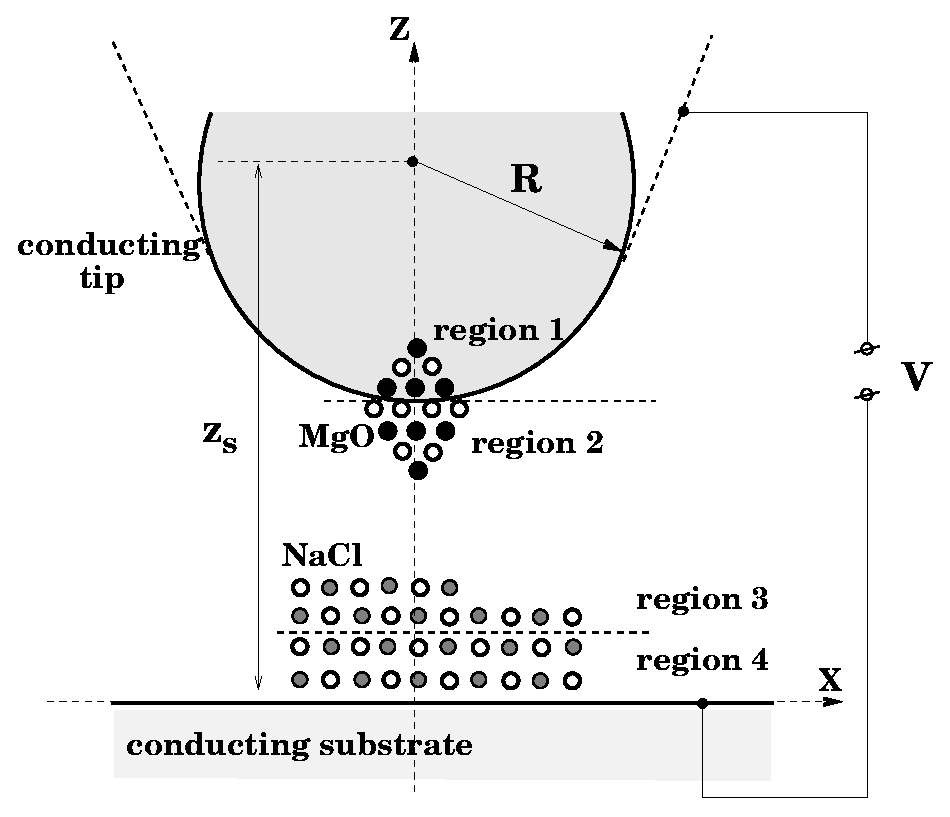
\includegraphics[%
  width=10cm]{xfig.model.eps}\end{center}


\caption{Example schematic picture of the microscopic model used to simulate
the interaction between the tip and the sample. \label{Tip_surf_schem}}
\end{figure}


The program itself is designed to calculate the interactions in systems
similar to that shown in fig. \ref{Tip_surf_schem}, with an atomistic
nano-tip embedded in a conducting macroscopic sphere interacting with
an atomistic cluster on top of a metal substrate. This represents
a very common experimental setup in modern AFM experiments using conducting
tips to image thin insulating films on top of metal substrates. However,
the code is very flexible in the types of setup it can study. The
properties of insulating tips can be easily investigated by removing
the conducting sphere from the system, and in fact the properties
of thin films alone can be studied by removing the tip completely
from the system. Some example input files at the end of this manual
show the variety of different setups that can be studied. 


\subsection{Electrostatic energy of a system of metals and charges}

Consider a set of \emph{finite} metallic conductors of arbitrary shape
and an arbitrary distribution of point charges $\{ q_{i}\}$ at the
points $\{\mathbf{r}_{i}\}$ anywhere in the free space outside the
conductors. We assume that the conductors which will hereafter be
designated by indices $m,m^{\prime}$ are kept at some \emph{fixed}
potentials $\phi_{m}$. These potentials are provided by the batteries. 

It is known from the standard textbooks (see e.g. Refs. \cite{Stratton},
\cite{Landau-8}, \cite{Jackson}) how to calculate the energy accumulated
in the electrostatic field $\mathbf{E}$ created by point charges
and metals. Using the total energy of the field, $U=\frac{1}{8\pi}\int_{V}\mathbf{E}^{2}d\mathbf{r}$
(the integral is taken over the volume $V$ outside the metals since
inside those the field $\mathbf{E}=0$) and applying the Poisson equation
for the field, one gets:

\begin{equation}
U=\frac{1}{2}\sum_{i}\, q_{i}\phi(\mathbf{r}_{i})+\frac{1}{2}\sum_{m}\, Q_{m}\phi_{m}\label{2}\end{equation}
 where the first sum is taken over all point charges whereas the second
one over all conductors. $Q_{m}=-\frac{1}{4\pi}\int\int_{S_{m}}\,\frac{\partial\phi}{\partial n}ds$
is the charge on the metal $m$, where the integral is performed over
the surface $S_{m}$ of the metal. Note that the surface integral
over a remote surface at infinity (which is surrounding all the metals
and the point charges) vanishes due to rapid decrease of the potential
to zero there \cite{Landau-8}. Therefore, this derivation is not
valid for infinite metals for which this assumption is not correct
(e.g. a charged infinite metal conductor). We also note in passing
that according to classical theory, the charge is distributed at the
surface, i.e. it does not penetrate into the bulk of the metal; quantum
theory \cite{Finnis-1}, \cite{Finnis-2}, \cite{Garcia-Bagus} gives
a certain distribution of the surface charge in the direction to the
bulk. 

The result of Eq. (\ref{2}) has a very simple physical meaning: every
charge $q$ at the point $\mathbf{r}_{q}$ (either a point charge
outside the metals or the distributed charge on a metal surface) gets
energy $\frac{1}{2}q\phi(\mathbf{r}_{q})$ where the factor $\frac{1}{2}$
is needed to avoid double counting. Note that the potential $\phi(\mathbf{r})$
is produced both by the metals (i.e. by the distributed charges on
their surfaces) and by the point charges. Note also that both the
potential $\phi(\mathbf{r}_{i})$ on point charges and the charges
$Q_{m}$ on the metals are unknown and should be calculated by solving
the Poisson equation. The effect of the metals comes into play via
the boundary conditions and the charges $Q_{m}$.

In order to calculate the electrostatic force imposed on any of the
conductors, we use the method essentially similar to the one of Ref.
\cite{Landau-8} where an arbitrary distribution of metals is considered
without point charges. The force is obtained by differentiating the
energy with respect to the corresponding position of the metal of
interest. It is shown in Ref. \cite{Landau-8} that the same expression
for the force is obtained in the cases of fixed potentials or fixed
charges on the metals. This, however, is not the case if the point
charges are present. Indeed, let us move some metal by the vector
$\delta\mathbf{r}$. The work $\delta A=-\mathbf{F}\delta\mathbf{r}$
is done by the external force against the force $\mathbf{F}$ imposed
on the conductor. When the conductor is moved to the new position,
the potential $\phi(\mathbf{r})$ in the system will change by $\delta\phi(\mathbf{r})$.
The potential on any metal $m$ will no longer be equal to the fixed
value $\phi_{m}$ so that there should be some charge flow between
the connected conductors to maintain the potential on them. Therefore,
some work $\delta A$ will be spent in changing the potential energy
of the field (given by Eq. (\ref{2})) by the amount \[
\delta U=\frac{1}{2}\sum_{i}\, q_{i}\delta\phi(\mathbf{r}_{i})+\frac{1}{2}\sum_{m}\,\phi_{m}\delta Q_{m}\]
and some work $\delta A_{b}$ is done in transfering charge \emph{between}
the conductors. The latter work $\delta A_{b}$ is done by the batteries
(as the charge flows via the battery from one conductor to another)
and so should be taken with the minus sign: $\delta A=-\delta A_{b}+\delta U$.
Alternatively, one could think of the batteries being incorporated
into the system; in that case it would mean that the work done by
the batteries would reduce the total potential energy of the whole
system. 

Let $\delta Q_{m}$ be the change of the charge on the conductor $m$
in the discussing process. Then the work $\delta A_{b}=\sum_{m}\phi_{m}\delta Q_{m}$
(cf. Eq. (2.5) in Ref. \cite{Landau-8}). Indeed, since $\sum_{m}\delta Q_{m}=0$,
this is the work needed to distribute the zero charge initially stored
at infinity (where the potential is zero) between different metals
by transferring the amounts $\delta Q_{m}$ to the each metal $m$.
Using the above given expressions, we obtain: \[
\delta A\equiv-\mathbf{F}\delta\mathbf{r}=-\sum_{m}\phi_{m}\delta Q_{m}+\delta U\]
so that the final expression for the force imposed on the displaced
metal becomes\begin{equation}
\mathbf{F}=-\frac{\partial U^{eff}}{\partial\mathbf{r}}\label{force}\end{equation}
with the \emph{effective energy} (or the total potential energy of
the whole system which includes the batteries as well) defined as:
\begin{equation}
U^{eff}=\frac{1}{2}\sum_{i}\, q_{i}\phi(\mathbf{r}_{i})-\frac{1}{2}\sum_{m}\, Q_{m}\phi_{m}\label{eff-energy}\end{equation}



\subsection{Tip-surface Interaction}

In order to calculate the force imposed on the tip we used the following
expression for the total energy of the system: \begin{equation}
U=\frac{1}{2}\sum_{ij}\,^{\prime}v_{ij}+U_{vdW}+U_{el}\label{1}\end{equation}
where $v_{ij}$ is the interatomic potential between atoms $i,j$.
This interaction energy is a function of both the tip position $z_{s}$
and the coordinates $\mathbf{r}_{i}$ of all atoms (and shells) involved.
The energy $U_{vdW}$ represents the van der Waals interaction between
the macroscopic tip and substrate and depends only on the tip height
$z_{s}$ with respect to the substrate (see Fig. 1). Note that in
the present model the macroscopic van der Waals interaction does not
effect atomic positions.

The last term in Eq. (\ref{1}) represents the total electrostatic
energy of the whole system. We assume that the Coulomb and covalent
interactions between all atoms is included in the first term in Eq.
(\ref{1}) and hence should be excluded from $U_{el}$. Therefore,
the energy $U_{el}$ includes the interaction of the atoms in the
system with the macroscopic tip and substrate. As has been demonstrated,
the correct electrostatic energy should incorporate the work done
by the battery to maintain the constant potential on the electrodes.
It can be written in the following form: \begin{equation}
U_{el}=-\frac{1}{2}Q^{(0)}V+\sum_{i}q_{i}\phi^{(0)}(\mathbf{r}_{i})+\frac{1}{2}\sum_{i,j}q_{i}q_{j}\phi_{ind}(\mathbf{r}_{i},\mathbf{r}_{j})\label{el-energy}\end{equation}
Here $V$ is the potential difference applied to the metal electrodes.
Without loss of generality, one can choose the potential $\phi$ on
the metal plane to be zero, so that the potential on the macroscopic
part of the tip will be $\phi=V$. We also note that the substrate
is considered in the limit of a sphere of a very big radius $R^{\prime}\gg R$
since the metal electrodes formally cannot be infinite. The charge
on the tip \emph{without} charges outside the metals (i.e. when there
are only bare electrodes and the polarization effects can be neglected)
is $Q^{(0)}$ and the electrostatic potential of the bare electrodes
anywhere outside the metals is $\phi^{(0)}(\mathbf{r})$. The charge
$Q^{(0)}$ and the potential $\phi^{(0)}(\mathbf{r})$ depend only
on the geometry of the capacitor formed by the two electrodes and
on the bias $V$. The charge $Q^{(0)}$ can be calculated from the
potential $\phi^{(0)}(\mathbf{r})$ as follows \cite{Landau-8}: $Q^{(0)}=-\frac{1}{4\pi}\int\int\,\frac{\partial\phi^{(0)}}{\partial n}ds$
where the integration is performed over the entire surface of the
macroscopic part of the tip with the integrand being the normal derivative
of the potential $\phi^{(0)}(\mathbf{r})$; the normal $\mathbf{n}$
is directed outside the metal. Summation in the second term of Eq.
(\ref{el-energy}) is performed over the atoms and shells of the sample
and those of the tip apex which are represented by point charges $q_{i}$
at positions $\mathbf{r}_{i}$. 

Finally, $\phi_{ind}(\mathbf{r},\mathbf{r}^{\prime})$ in Eq. (\ref{el-energy})
is the potential at \emph{$\mathbf{r}$} due to image charges \emph{induced}
on all the metals by a unit point charge at $\mathbf{r}^{\prime}$.
This function is directly related to the Green function \textbf{$G(\mathbf{r},\mathbf{r}^{\prime})$}
of the Laplace equation, \textbf{$\phi_{ind}(\mathbf{r},\mathbf{r}^{\prime})=G(\mathbf{r},\mathbf{r}^{\prime})-\frac{1}{\mid\mathbf{r}-\mathbf{r}^{\prime}\mid}$},
and is symmetric, i.e. $\phi_{ind}(\mathbf{r},\mathbf{r}^{\prime})=\phi_{ind}(\mathbf{r}^{\prime},\mathbf{r})$,
due to the symmetry of the Green function itself \cite{Jackson}.
The total potential at \textbf{$\mathbf{r}$} due to a net charge
induced on all conductors present in the system by all the point charges
$\{ q_{i}\}$, \begin{equation}
\phi_{ind}(\mathbf{r})=\sum_{i}q_{i}\phi_{ind}(\mathbf{r},\mathbf{r}_{i})\label{fi-ind-nwe}\end{equation}
 is the \emph{image potential}. Note that the last double summation
in Eq. (\ref{el-energy}) includes the $i=j$ term as well. This term
corresponds to the interaction of the charge $q_{i}$ with its own
polarization (similar to the polaronic effect in solid-state physics). 

The function $\phi_{ind}(\mathbf{r},\mathbf{r}^{\prime})$ and, therefore,
the image potential, $\phi_{ind}(\mathbf{r})$, together with the
potential $\phi^{(0)}(\mathbf{r})$ of the bare electrodes could be
calculated if we knew the exact Green function of the electrostatic
problem \begin{equation}
\Delta_{\mathbf{r}^{\prime}}G(\mathbf{r},\mathbf{r}^{\prime})=-4\pi\delta(\mathbf{r}-\mathbf{r}^{\prime})\label{Poisson}\end{equation}
with the corresponding boundary conditions ($G(\mathbf{r},\mathbf{r}^{\prime})=0$
when $\mathbf{r}$ or $\mathbf{r}^{\prime}$ belong to either the
substrate or the tip surface) \cite{Jackson}. Therefore, given the
applied bias $V$, the geometric characteristics of the capacitor
and the positions $\{\mathbf{r}_{j}\}$ of the point charges $\{ q_{i}\}$
between the tip and sample, one can calculate the electrostatic energy
$U_{el}$. The problem is that the Green function for real tip-sample
shapes and arrangements is difficult to calculate. In this study we
use the planar-spherical geometry of the junction as depicted in Fig.
\ref{Tip_surf_schem}. 


\subsection{\label{charges_sol}Solution of the electrostatic problem of point
charges inside the sphere-plane capacitor}

First, let us consider the calculation of the potential $\phi^{(0)}(\mathbf{r})$
of the bare electrodes, i.e. the capacitor problem. We note that the
potential $\phi^{(0)}(\mathbf{r})$ satisfies the same boundary conditions
as the original problem, i.e. $\phi^{(0)}=0$ and $\phi^{(0)}=V$
at the lower and upper electrodes, respectively. The solution for
the plane-spherical capacitor is well known \cite{Smythe} and can
be given using the method of image charges. Since we will need this
solution for calculating forces later on, we have to give it here
in detail. It is convenient to choose the coordinate system as shown
in Fig. \ref{Tip_surf_schem}. Then it is easy to check that the following
two \emph{infinite} sequences of image charges give the potential
at the sphere and the metal plane as $V$ and zero respectively. The
first sequence is given by the image charges $\varsigma_{1}=RV$ and
then $\varsigma_{k+1}=\frac{\varsigma_{k}}{D_{k}}$ for $\forall k=1,2,\ldots$,
where the dimensionless constants $D_{k}$ are defined by the recurrence
relation $D_{k+1}=2\lambda-\frac{1}{D_{k}}$with $D_{1}=2\lambda$
and $\lambda=\frac{z_{s}}{R}>1$, $z_{s}$ being the distance between
the sphere centre and the plane (Fig. \ref{Tip_surf_schem}). The
point charges $\{\varsigma_{k}\}$ are all inside the sphere along
the normal line passing through the sphere centre. Their $z$-coordinates
are as follows: $z_{1}=z_{s}$ and $z_{k+1}=R\left(\lambda-\frac{1}{D_{k}}\right)=R(D_{k+1}-\lambda)$
for $\forall k=1,2,\ldots$. The second sequence of charges $\{\varsigma_{k}^{\prime}\}$
is formed by the images of the first sequence with respect to the
metal plane, i.e. $\varsigma_{k}^{\prime}=-\varsigma_{k}$ and $z_{k}^{\prime}=-z_{k}$.
An interesting point about the image charges $\{\varsigma_{k}\}$
is that they converge very quickly at the point $z_{\infty}=R\sqrt{\lambda^{2}-1}$
(i.e. $z_{k}\rightarrow z_{\infty}$ with $k\rightarrow\infty$) and
that $z_{k+1}<z_{k}$ for $\forall k$. This is because the numbers
$D_{k}$ converge rapidly to the limiting value $D_{\infty}=\lambda+\sqrt{\lambda^{2}-1}$
which follows from the original recurrent relation above, $D_{\infty}=2\lambda-\frac{1}{D_{\infty}}$.
Therefore, while calculating the potential $\phi^{(0)}(\mathbf{r})$,
one can consider the charges $\{\varsigma_{k}\}$ and $\{\varsigma_{k}^{\prime}\}$
explicitly only up to some $k=k_{0}-1$ and then sum up the rest of
the charges to infinity analytically to obtain the effective charge
$\varsigma_{\infty}=\sum_{k=k_{0}}^{\infty}\varsigma_{k}=\sum_{n=0}^{\infty}\frac{\varsigma_{k_{0}}}{D_{\infty}^{n}}=\frac{\varsigma_{k_{0}}D_{\infty}}{D_{\infty}-1}$
to be placed at $z_{\infty}$. This can be used \emph{instead} of
the rest of the series: \begin{equation}
\phi^{(0)}(\mathbf{r})=\sum_{k=1}^{k_{0}}\overline{\varsigma}_{k}\left(\frac{1}{|\mathbf{r}-\mathbf{r}_{\varsigma_{k}}|}-\frac{1}{|\mathbf{r}-\widehat{\sigma}\mathbf{r}_{\varsigma_{k}}|}\right)\label{fi-0}\end{equation}
where $\overline{\varsigma}_{k}=\varsigma_{k}$ for $k<k_{0}$ and
$\overline{\varsigma}_{k_{0}}=\varsigma_{\infty}$; then, $\mathbf{r}_{\varsigma_{k}}=(0,0,z_{k})$
is the position vector of the charge $\varsigma_{k}$ and $\mathbf{r}_{\varsigma_{k}^{\prime}}=\widehat{\sigma}\mathbf{r}_{\varsigma_{k}}=(0,0,-z_{k})$
is the position of the charge $\varsigma_{k}^{\prime}$ ($\widehat{\sigma}$
means reflection with respect to the substrate surface $z=0$). To
find the charge $Q^{(0)}$ which is also needed for the calculation
of the electrostatic energy, Eq. (\ref{el-energy}), one should calculate
the normal derivative of the potential $\phi^{(0)}(\mathbf{r})$ on
the sphere and then take the corresponding surface integral (see above).
However, it is useful to recall that the total charge induced on the
metal sphere due to an external charge is equal exactly to the image
charge inside the sphere \cite{Landau-8}, \cite{Jackson}. Therefore,
one immediately obtains: \begin{equation}
Q^{(0)}=\sum_{k=1}^{k_{0}}\overline{\varsigma}_{k}\label{Q_0}\end{equation}
Note that the potential $\phi^{(0)}(\mathbf{r})$ and the charge $Q^{(0)}$
depend on the position $z_{s}$ of the sphere \emph{indirectly} via
the charges $\varsigma_{k}$ and their positions $\mathbf{r}_{\varsigma_{k}}$
according to the recurrent expressions above. Therefore, one has to
be careful when calculating the contribution to the force imposed
on the tip due to bias V (i.e. when differentiating $\phi^{(0)}(\mathbf{r})$
and $Q^{(0)}$ in Eq. (\ref{el-energy})). 

Now we turn to the calculation of the function $\phi_{ind}(\mathbf{r},\mathbf{r}^{\prime})$
in Eq. (\ref{el-energy}). This function corresponds to the image
potential at a point $\mathbf{r}$ due to a unit charge at $\mathbf{r}^{\prime}$.
This potential is to be defined in such a way that together with the
direct potential of the unit point charge, it should be zero on both
electrodes (the boundary condition for the Green function). Thus,
let us consider a unit charge $q=1$ at $\mathbf{r}_{q}$ somewhere
outside the metal electrodes as shown in Fig. \ref{2spheres}.%
\begin{figure}[!ht]
\begin{center}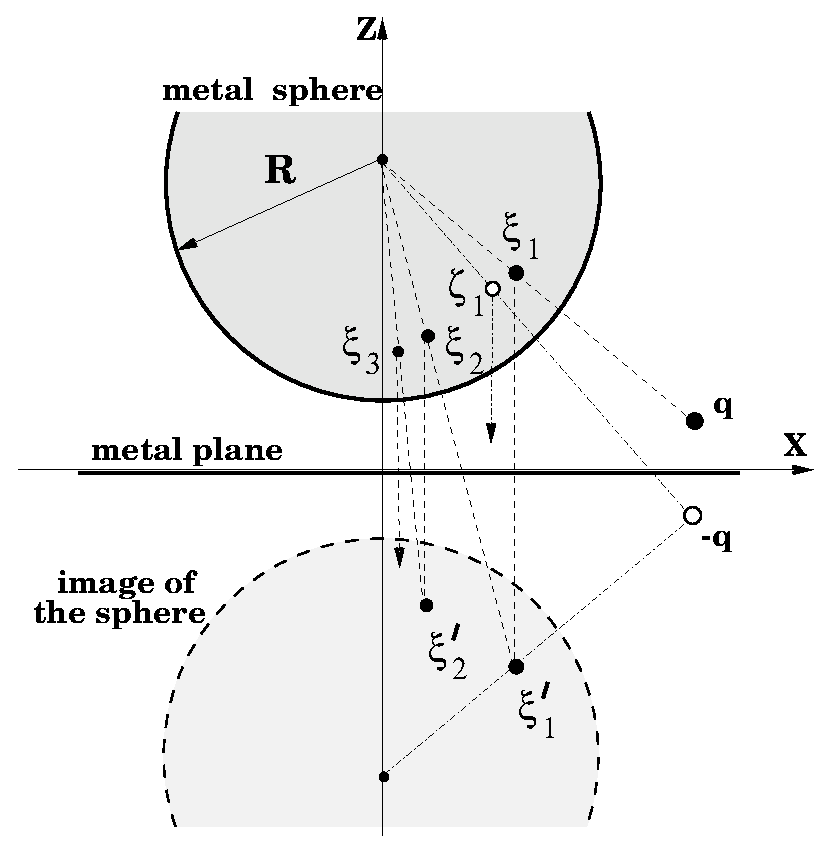
\includegraphics[%
  width=10cm]{xfig.image.eps}\end{center}


\caption{Construction of image charges in the sphere-plane capacitor system
due to one charge $q$ outside the metals.\label{2spheres}}
\end{figure}
  We first create the direct image $-q$ of this charge with respect
to the plane at the point $\mathbf{r}_{q}^{\prime}=\widehat{\sigma}\mathbf{r}_{q}$
to maintain zero potential at the plane. Then, we create images of
the two charges, $q=1$ and $-q=-1$, with respect to the sphere to
get two image charges $\xi_{1}=-\frac{R}{|\mathbf{r}_{q}-\mathbf{R}_{s}|}$
and $\zeta_{1}=\frac{R}{|\widehat{\sigma}\mathbf{r}_{q}-\mathbf{R}_{s}|}$,
as shown in Fig. \ref{2spheres} where $\mathbf{R}_{s}=(0,0,z_{s})$.
These image charges are both inside the sphere by construction and
their positions can be written down using a vector function $\mathbf{f}(\mathbf{r})=\mathbf{R}_{s}+R^{2}\frac{\mathbf{r}-\mathbf{R}_{s}}{|\mathbf{r}-\mathbf{R}_{s}|^{2}}$
as follows: $\mathbf{r}_{\xi_{1}}=\mathbf{f}(\mathbf{r}_{q})$ and
$\mathbf{r}_{\zeta_{1}}=\mathbf{f}(\widehat{\sigma}\mathbf{r}_{q})$.
Now the potential at the surface will be zero. At the next step we
construct the images $\xi_{1}^{\prime}=-\xi_{1}$ and $\zeta_{1}^{\prime}=-\zeta_{1}$
of the charges $\xi_{1}$ and $\zeta_{1}$ in the plane at points
$\widehat{\sigma}\mathbf{r}_{\xi_{1}}$ and $\widehat{\sigma}\mathbf{r}_{\zeta_{1}}$
respectively, to get the potential at the plane also zero. This process
is continued and in this way two infinite sequences of image charges
are constructed, which are given by the following recurrence relations:\begin{equation}
\left\{ \begin{array}{c}
\xi_{k+1}=\xi_{k}\frac{R}{|\widehat{\sigma}\mathbf{r}_{\xi_{k}}-\mathbf{R}_{s}|}\\
\mathbf{r}_{\zeta_{k+1}}=\mathbf{f}(\widehat{\sigma}\mathbf{r}_{\xi_{k}})=\mathbf{R}_{s}+R^{2}\frac{\widehat{\sigma}\mathbf{r}_{\xi_{k}}-\mathbf{R}_{s}}{|\widehat{\sigma}\mathbf{r}_{\xi_{k}}-\mathbf{R}_{s}|^{2}}\end{array}\right.\label{1st-seq}\end{equation}
where $k=1,2,\ldots$ and similarly for the $\zeta$-sequence. Note,
however, that the two sequences start from different initial charges.
Namely, the $\xi$-sequence starts from the original charge $q$ while
the $\zeta$-sequence from its image in the plane $-q$. The two sequences
$\{\xi_{k}\}$ and $\{\zeta_{k}\}$ are to be accompanied by the other
two sequences $\{\xi_{k}^{\prime}\}$ and $\{\zeta_{k}^{\prime}\}$
which are the images of the former charges with respect to the plane.
The four sequences of the image charges and the charges $q$ and $-q$
provide the correct solution for the problem formulated above since
they produce the potential which is the solution of the corresponding
Poisson equation and, at the same time, is zero both on the metal
sphere and the metal plane. 

It is useful to study the convergence properties of the sequences
of image charges. To simplify the notations, let us assume that the
original charge is in the $xz$-plane. Then it follows from Eq. (\ref{1st-seq})
that $x_{\xi_{k+1}}<x_{\xi_{k}}$ . It is also seen that $x_{\xi_{k}}\rightarrow0$
and $z_{\xi_{k}}\rightarrow z_{\infty}=R\sqrt{\lambda^{2}-1}$ (see
above) as $k\rightarrow\infty$ and the same for the $\zeta$-sequence.
This means that the image charges inside the sphere move towards the
vertical line passing through the centre of the sphere and finally
converge at the same point $z_{\infty}$. This is the same behaviour
we observed for charges in the capacitor problem at the beginning
of this subsection (see Fig. \ref{2spheres}). In fact, the calculation
clearly shows a very fast convergence so that we can again sum up
the series of charges from some $k=k_{0}$. Thus, the image potential
at a point $\mathbf{r}$ due to the unit charge at $\mathbf{r}_{q}$
is: \begin{equation}
\phi_{ind}(\mathbf{r},\mathbf{r}_{q})=-\frac{1}{\mathbf{r}-\widehat{\sigma}\mathbf{r}_{q}}+\sum_{k=1}^{k_{0}}\left[\overline{\xi}_{k}\left(\frac{1}{|\mathbf{r}-\mathbf{r}_{\xi_{k}}|}-\frac{1}{|\mathbf{r}-\widehat{\sigma}\mathbf{r}_{\xi_{k}}|}\right)+\overline{\zeta}_{k}\left(\frac{1}{|\mathbf{r}-\mathbf{r}_{\zeta_{k}}|}-\frac{1}{|\mathbf{r}-\widehat{\sigma}\mathbf{r}_{\zeta_{k}}|}\right)\right]\label{Fi-ind}\end{equation}
where $\overline{\xi}_{k}=\xi_{k}$ for $k<k_{0}$ and $\overline{\xi}_{k_{0}}=\xi_{\infty}=\xi_{k_{0}}\frac{D_{\infty}}{D_{\infty}-1}$,
and similarly for the $\zeta$-sequence. Here $D_{\infty}$ is the
geometrical characteristic of the capacitor introduced at the beginning
of this subsection. 

As it has been already mentioned in Section 2.1, the function $\phi_{ind}(\mathbf{r},\mathbf{r}_{q})$
must be symmetric with respect to the permutation of its two variables.
It is not at all obvious that this is the case since the meaning of
its two arguments in Eq. (\ref{Fi-ind}) is rather different. Nevertheless,
we show in ref. \cite{our_imageforce} that the function $\phi_{ind}(\mathbf{r},\mathbf{r}_{q})$
is symmetric.


\subsection{The calculation of the total force acting on the tip}

In order to calculate the total force acting on the tip, one has to
differentiate the total energy, Eq. (\ref{1}), with respect to the
position of the sphere, $\mathbf{R}_{s}$. Since we are interested
only in the force acting in the $z$-direction, it is sufficient to
study the dependence of the energy on $z_{s}$. There will be three
contributions to the force. The second contribution to the force comes
from the van der Waals interaction \cite{French}. Finally, the interatomic
interactions lead to a force which is calculated by differentiating
the shell-model energy (the first term in Eq. (\ref{1})). Therefore, 

\begin{equation}
F_{tip}=-\frac{dU_{sh}}{dz_{s}}-\frac{dU_{vdW}}{dz_{s}}-\frac{dU_{el}}{dz_{s}}\label{force-1}\end{equation}
where $U_{sh}=\frac{1}{2}\sum_{ij}\,^{\prime}v_{ij}$ is the shell
model energy. We recall that the summation here is performed over
all atoms in regions 1 to 4. Only positions of the atoms in region
1 depend directly on $z_{s}$ since atoms in other regions are allowed
to relax. However, their equilibrium positions, $\mathbf{r}_{i}^{(0)}$,
determined by the minimisation of the energy of Eq. (\ref{1}), will
depend \emph{indirectly} on $z_{s}$ at equilibrium, $\mathbf{r}_{i}^{(0)}=\mathbf{r}_{i}^{(0)}(z_{s})$.
Then, we also recall that the electrostatic energy, $U_{el}$, depends
only on positions of atoms, as well as on the tip position $z_{s}$.

Let us denote the positions of atoms by a vector \textbf{$\mathbf{x}=(\mathbf{r}_{1},\mathbf{r}_{2},\ldots)$}.
The total energy $U=U(\mathbf{x},z_{s})$, where the direct dependence
on $z_{s}$ comes from relaxed tip atoms of the shell model energy,
$U_{sh}$, and from the electrostatic energy, $U_{el}$. In equilibrium
the total energy is a minimum:\begin{equation}
\left(\frac{\partial U}{\partial\mathbf{x}}\right)_{z_{s}}=0\label{equi}\end{equation}
where the derivatives are calculated at a given fixed tip position
$z_{s}$. Let \textbf{$\mathbf{x}_{0}=(\mathbf{r}_{1}^{(0)},\mathbf{r}_{2}^{(0)},\ldots)$}
be the solution of Eq. (\ref{equi}). Then, since $\mathbf{x}_{0}=\mathbf{x}_{0}(z_{s})$,
we have for the force: \begin{equation}
F_{tip}=-\frac{dU(\mathbf{x}_{0}(z_{s}),z_{s})}{dz_{s}}=-\left(\frac{\partial U}{\partial\mathbf{x}_{0}}\right)_{z_{s}}\frac{\partial\mathbf{x}_{0}}{\partial z_{s}}-\left(\frac{\partial U}{\partial z_{s}}\right)_{\mathbf{x}_{0}}=-\left(\frac{\partial U}{\partial z_{s}}\right)_{\mathbf{x}_{0}}\label{fin-prelast}\end{equation}
where we have used Eq. (\ref{equi}). This result can be simplified
further. Indeed, the partial derivative of the shell-model energy,
$-\frac{\partial U_{sh}}{\partial z_{s}}$, is equal to the sum of
all $z$-forces acting on atoms in region 1 due to all shell-model
interactions, since only these atoms are responsible for the dependence
on $z_{s}$ in the energy $U_{sh}$. Therefore, finally we have: \begin{equation}
F_{tip}=\sum_{i\in1}\left(F_{iz}^{(sh)}\right)_{\mathbf{x}_{0}}-\frac{dU_{vdW}}{dz_{s}}-\left(\frac{\partial U_{el}}{\partial z_{s}}\right)_{\mathbf{x}_{0}}\label{fin-force}\end{equation}
where the first summation runs only over fixed tip atoms. Thus, in
order to calculate the force imposed on the tip at a given tip position
$z_{s}$, one has to relax the positions of atoms using the \emph{total
energy} of the system, $U_{sh}+U_{el}$. Then calculate the shell-model
force, $F_{iz}^{(sh)}$, acting on every fixed tip atom in the $z$-direction
as well as the electrostatic contribution to the force given by the
last term in Eq. (\ref{fin-force}). The van der Waals force between
macroscopic tip and sample does not depend on the geometry of atoms
and can be calculated just once for every given $z_{s}$. 


\subsubsection{Definition of the Instantaineous Force on the Tip (for MD)}

In the case where the system is dynamic and atoms are given kinetic
energy, it becomes obvious that the definition of the tip force given
in the previous section no longer holds, since the forces on free
atoms are no longer zero: $\frac{\partial U}{\partial\mathbf{r}}\neq0$.
It is also clear that because of this when the entire tip is far from
the surface, region 1 will experience large fluctuations in force
of Eq. (\ref{fin-prelast}) due to oscillating other tip atoms belonging
to the adjacent region 2. Moreover, these fluctuations will not decay
with the distance from the surface which is in clear contradiction
with what one would expect from the tip force which is physically
due to the interaction with the surface. Even for a completely isolated
tip the force fluctuations are large although, since region 2 atoms
vibrate around equilibrium positions, the average force fluctuates
around zero value. Hence, we conclude that the final form of Eq. (\ref{fin-prelast})
can only be used for calculating the force in mechanical equilibrium
or when calculating the \emph{average} force during MD simulations.
If we are interested in the actual \emph{fluctuations} of the tip
force for any given tip position $Q$, Eq. (\ref{fin-prelast}) cannot
be applied. 

What is needed in order to provide an alternative expression for the
tip force which would work for both static and dynamic situations,
is the definition of an \emph{instantaneous} force for arbitrary positions
of atoms in the junction. At first, one might be tempted to define
the tip force as the partial derivative, $-\frac{\partial U}{\partial Q}$,
of the total system energy $U$ with respect to tip height $Q$ at
\emph{arbitrary} positions of atoms, $\mathbf{r}$, which are allowed
to relax. However, this definition, as can easily be seen, leads to
the same expression for the force, Eq. (\ref{fin-prelast}), because
only atoms in region 1 depend explicitly on $Q$, and thus cannot
be accepted.

In order to obtain an appropriate definition of the tip force, we
invoke a general non-equilibrium microscopic consideration in which
the total Hamiltonian of the {}``tip - surface'' system was shown
\cite{KANT_QM_coarse-grained} to be split as follows:

\begin{equation}
H=H_{s}+\Phi+H_{T}\label{Hamiltonian}\end{equation}
Here $H_{s}$ is the sum of the independent \emph{microscopic} Hamiltonians
of the isolated surface and the isolated tip. Either of those contains
kinetic and potential energies of the constituent atoms. Note that
atomic positions in the tip part of $H_{s}$ are defined \emph{relatively}
to the fixed part of the tip (e.g. using internal coordinates). Note
also that there is \emph{no} interaction between atoms in the surface
and in the tip included in $H_{s}$. This interaction is completely
included in the second term, $\Phi$, in Eq. (\ref{Hamiltonian}).
Since absolute positions of the tip atoms are to be used while specifying
the tip-surface interaction, $\Phi$ depends both on the atomic positions
and the tip height, $Q$. As the distance between the tip and surface
increases, the tip-surface interaction $\Phi$ tends to zero. Finally,
$H_{T}$ is the \emph{macroscopic} Hamiltonian of the tip which contains
kinetic and elastic energy of the cantilever as well as the excitation
term. It depends exclusively on $Q$ and also contributes to the conservative
part of the tip force. Since we are not interested in the conservative
contribution (it does not contribute to the force fluctuations), it
will be ignored in this presentation. Note that the interaction term,
$\Phi$ can always be defined for arbitrary complex many body interactions
between the tip and surface, and thus our treatment is not limited
to systems consisting only of pairwise interactions. 

It then follows from the microscopic non-equilibrium theory that the
instantaneous microscopic force acting on the tip (which completely
includes the \emph{stochastic} contribution due to atomic vibrations
\cite{NC-AFM_book_my-contribution}) should be defined as follows: 

\begin{equation}
F=-\frac{\partial\Phi}{\partial Q}=f_{13}+f_{23}\label{force-correct-1}\end{equation}
where $f_{ij}$ is the sum of the vertical forces acting on all the
atoms in region $i$ due to all of the atoms in region $j$ \cite{tip-force-def-Tom}.
The important difference with the static definition of Eq. (\ref{fin-prelast})
is that the force is defined as the partial derivative of the \emph{interaction}
energy $\Phi$ rather than the \emph{total} energy $U$. We see that
the microscopic force on the tip is given as the sum of the \emph{partial
forces} on \emph{all} atoms of the tip due to all of the atoms in
the surface. 

The above expression does not require that the system is in equilibrium,
and, due to partitioning of the total Hamiltonian discussed above,
Eq. (\ref{Hamiltonian}), it naturally tends to zero when the tip
and the surface are separated. It is also equivalent to the static
definition (\ref{fin-prelast}) if the system is in equilibrium. Indeed,
since $f_{21}=-f_{12}$, $f_{22}=0$ and $f_{11}=0$ at any given
time $t$, we can also write $F$ as \begin{equation}
F=\left(f_{23}+f_{22}+f_{21}\right)+\left(f_{13}+f_{12}+f_{11}\right)\label{final-force}\end{equation}
The first term (all three terms in the first brackets) is equal to
the sum of the total forces acting on atoms in region 2 due to all
other atoms in the system; it is equal to zero in mechanical equilibrium.
Thus, in this case $F$ reduces to the second term (the second brackets)
which is equal to the sum of forces acting on the frozen atoms of
the tip comprising region 3 which is indeed identical to that given
by Eq. (\ref{fin-prelast}).

In practical calculations the expression for the force (\ref{force-correct-1})
is not very convenient since it requires calculation of partial forces
due to different regions to be recorded during each simulation step.
The equivalent expression (\ref{final-force}), which will be referred
to as the \emph{dynamic} definition of the tip force (as opposed to
the \emph{static} definition of Eq. (\ref{fin-prelast})) is much
more convenient since it contains the sum of total forces acting on
\emph{all} atoms of the tip. This expresion is used in the code when
calculating the continuous force on the tip during a simulaion. 


\subsection{Interatomic Potentials}


\subsubsection{Force Field}

The potential energy surface of the system is modelled by the following
force field:

\[
E=\sum_{b}^{N_{b}}K_{b}(b-b_{0})^{2}+\sum_{\theta}^{N_{\theta}}K_{\theta}(\theta-\theta_{0})^{2}+\sum_{\phi}^{N_{\phi}}K_{\phi}\left[1+\cos(n\phi-\phi_{0})\right]+\sum_{\chi}^{N_{\chi}}K_{\chi}\left[1+\cos(n\chi-\chi_{0})\right]\]


\begin{equation}
+\sum_{ij}\frac{q_{i}q_{j}}{\varepsilon r_{ij}}+\sum_{ij}C_{ij}r_{ij}^{-n_{ij}}+\sum_{ij}A_{ij}e^{-\frac{r_{ij}}{\rho_{ij}}}\label{force-field}\end{equation}


The first four terms in the above expression apply to the many body
interactions in the system and summations only apply to the specified
interactions, with the parameters suplied by the user and the values
of the internal coordinates (bond lengths $b$, angles between bonds
$\theta$, torsions about bonds $\phi$ and out-of-plane angles $\chi$)
calculated using the expressions in section 2.5.2. Many body interactions
are used to model covalently bonded crystals and organic molecules
in the system. 

The final three terms in the above expression are pairwise interactions,
and are summed over all pairs of atoms in the system (except those
exluded in covalent bond or angle interactions). The program implements
the Shell Model to calculate pairwise interactions, first introduced
in \cite{shell-dick}. In this scheme, atoms are represented by positively
charged cores connected to negatively charged shells by harmonic springs,
which represent nuclear and electron charge respectively. The equilibrium
distance between the core and shell is a representation of the electronic
polarization of that atom. Cores and shells of the same atom only
interact via the harmonic spring, however each atomic core and shell
interacts via colombic forces with all other cores and shells in the
system. 

Short range repulsive and Van de Waals forces are descibed by pairwise
Buckingham potentials (last two terms in the above expression), which
act only between shells. 


\subsubsection{Internal Coordinates}

The internal coordinates used to calculate the energy expressions
for many body intercations are described below. The internal coordinates
are defined between the cores, and not shells, of atoms. 

The length of a bond between two atoms in a molecule is straightforward
to visualise, and is simply calculated as the magnitude of the vector
(\textbf{r}) between the two atoms (\textit{i} and \textit{j}) (figure
\ref{bond-length}).

%
\begin{figure}[!ht]
\begin{center}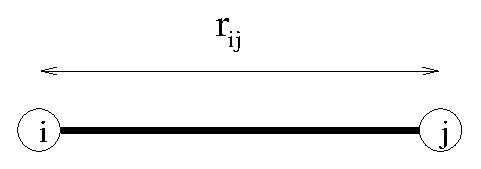
\includegraphics[%
  width=4cm]{bond.eps}~~~~~~$b_{ij}=\left|\underline{r}_{ij}\right|=\sqrt{(x_{j}-x_{i})+(y_{j}-y_{i})+(z_{j}-z_{i})}$\end{center}


\caption{Bond Length\label{bond-length}}
\end{figure}


The angle between two adjacent bonds in a molecule, or the angle formed
by the three nuclei \textit{i}, \textit{j} and \textit{k} is calculated
using the dot product of the two vectors from \textit{j} to \textit{i}
($r_{ji}$) and \textit{j} to \textit{k} ($r_{jk}$) as shown in figure
\ref{bond-angle}.

%
\begin{figure}[!ht]
\begin{center}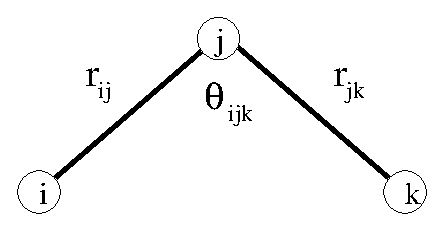
\includegraphics[%
  width=4cm]{angle.eps}~~~~~~$\theta_{ijk}=\arccos\left(\frac{\underline{r}_{ij}\bullet\underline{r}_{kj}}{\left|\underline{r}_{ij}\right|\left|\underline{r}_{kj}\right|}\right)$\end{center}


\caption{Bond Angle\label{bond-angle}}
\end{figure}


A torsion angle about a bond \textit{j} - \textit{k} is defined for
any four sequentially bonded atoms in a molecule, \textit{i}, \textit{j},
\textit{k} and \textit{l} and made by the angle between the planes
formed by the two angles \textit{$\theta_{ijk}$} and \textit{$\theta_{jkl}$}
(Figure 3.4). The torsion angle is then calculated by taking the dot
product of the normal unit vectors of these two planes, each of which
is calculated from the vector cross products of $\underline{r}_{ji}$
with $\underline{r}_{jk}$ and of $\underline{r}_{jk}$ with $\underline{r}_{lk}$
as shown in figure \ref{torsion}. 

%
\begin{figure}[!ht]
\begin{center}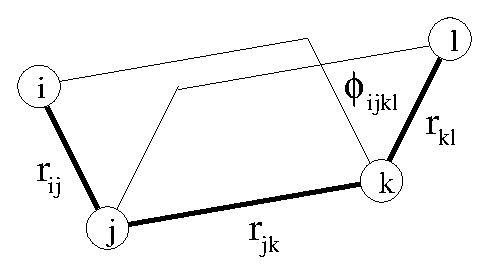
\includegraphics[%
  width=4cm]{torsion.eps}~~~~~~$\phi_{ijkl}=\arccos\left[\frac{(\underline{r}_{ij}\times\underline{r}_{kj})\bullet(\underline{r}_{kj}\times\underline{r}_{kl})}{\left|\underline{r}_{ij}\times\underline{r}_{kj}\right|\left|\underline{r}_{kj}\times\underline{r}_{kl}\right|}\right]$\end{center}


\caption{Torsion Angle\label{torsion}}
\end{figure}


An out-of-plane angle needs to be defined when an atom in a molecule
is bonded to just three other atoms (central atom \textit{i} bonded
to atoms \textit{j}, \textit{k} and \textit{l}), and the out-of-plane
angle ($\chi$) is defined as the average of the three improper torsions
formed by the interaction. 

The improper torsion definition uses the torsion angle expression
above to calculate the torsion angle formed by the atoms \textit{i}
- \textit{k} - \textit{l} - \textit{j}, which is the angle between
the plane formed by the three atoms \textit{i}, \textit{k}, \textit{l}
and the plane formed the atoms \textit{k}, \textit{l} and the central
atom \textit{i}. It is so called improper as the torsion is about
two atoms that are not bonded together. 

The analytical derivatives of these expresions are used by the code
to calculate the gradients of the energy analytically, which allows
both MD and minimisation calculations to be performed efficiently.
The code also allows the forces on atoms calculated analytically to
be checked by a numerical interpolation of the energy (see section
4.2.13). 


\subsection{Constrained minimisation\label{Sec::constrains-theory}}

The code can perform constrained minimisation searches%
\footnote{Formally, constraines can also be used during MD runs, but those should
be done with care and generally we do not recommend this approach
unless you know what you are doing.%
}. A general structure implemented actually allows for very sophisticated
nonlinear constraines, but those in general require some additional
coding which is desribed in some detail in the corresponding routines
as documented in Table \ref{Table::constraines}:%
\begin{table}[!ht]
\begin{tabular}{|c|c|c||c|}
\hline 
routine&
file&
comment&
extra coding?\tabularnewline
\hline
\hline 
\texttt{constraints()}&
\texttt{inval.f}&
reading from input file; setting up&
Yes\tabularnewline
\hline 
\texttt{check\_constr()}&
\texttt{inval.f}&
checking all constraines for consistency&
May be\tabularnewline
\hline 
\texttt{force\_conv\_3\_1()}&
\texttt{shell.f}&
converts forces \texttt{fx},\texttt{fy},\texttt{fz} => 1 dim vector&
Yes\tabularnewline
\hline 
\texttt{coord\_constr()}&
\texttt{shell.f}&
deals with redundant coordinates&
Yes\tabularnewline
\hline
\texttt{conv\_1\_3()}&
\texttt{shell.f}&
converts coordinates to \texttt{x},\texttt{y},\texttt{z} from 1 dim
vector&
No\tabularnewline
\hline
\texttt{conv\_3\_1()}&
\texttt{shell.f}&
converts coordinates \texttt{x},\texttt{y},\texttt{z} => 1 dim vector&
No\tabularnewline
\hline
\texttt{do\_restart()}&
\texttt{restart.f}&
dumps an input RST file&
Yes\tabularnewline
\hline
-&
\texttt{constr.inc}&
memory storage/definitions&
Yes\tabularnewline
\hline
\end{tabular}


\caption{Routines and the corresponding files responsible for the interface
dealing with imposed constraines. The last column states if any extra
coding is required when an additional constraint is to be added.\label{Table::constraines}}
\end{table}
We shall first explain the main ideas of very general constraints;
then linear constrains which are implemented in a rather general way
in the code will be discussed specifically. 


\subsubsection{How constrains are dealt with in the code}

Constraints are dealt with in the following general way: every constrained
equation specifies a single atomic coordinate of some atom (say, coordinate
$x$ of atom 3, i.e. $x_{3}$) which is a function of other coordinates
of the same and/or some other atoms, i.e. $x_{3}=\xi(y_{3},z_{1},x_{2})$.
The coordinate $x_{3}$ is then made \emph{redundand} and is removed
from the optimisation space. The consequence of this is that, when
calculating the {}``force'' in the optimisation space associated
with other coordinates which are involved in the given constraint,
there will be an additional contribution due to the constraint. In
the example above coordinates $y_{3}$, $z_{1}$ and $x_{2}$ are
involved, so that the energy \[
E=E(x_{1},y_{1},z_{1},x_{2},y_{2},z_{2},x_{3}(y_{3},z_{1},x_{2}),y_{3},z_{3})\equiv\widetilde{E}(x_{1},y_{1},z_{1},x_{2},y_{2},z_{2},y_{3},z_{3})\]
 is a function of all coordinates except for $x_{3}$. Therefore,
the {}``force'' associated with this coordinate is not needed during
optimisation. However, e.g. the {}``force'' associated with $y_{3}$
becomes:\[
\widetilde{f}_{3y}=-\frac{\partial\widetilde{E}}{\partial y_{3}}=-\frac{\partial E}{\partial y_{3}}-\frac{\partial E}{\partial x_{3}}\frac{\partial x_{3}}{\partial y_{3}}=f_{3y}+f_{3x}\frac{\partial x_{3}}{\partial y_{3}}=f_{3y}+f_{3x}\frac{\partial\xi}{\partial y_{3}}\]
where $f_{3y}$ and $f_{3x}$ are the actual (physical) forces on
atom 3 in the $y$ and $x$ directions, respectively. These are calculated
routinely in the code irrespective of the constraints. The derivative
$\frac{\partial\xi}{\partial y_{3}}$ needed for the calculation of
the {}``force'' $\widetilde{f}_{3y}$ should be calculated analytically
for every particular constraint from the known function $\xi$ and
then coded in in the appropriate places. 

There is presently only one important limitation on the atoms involved
in constraints: a reduntand coordinate must be contained in only one
constraint; it is not allowed that it is a member of another constraint
as well. However, other coordinates are allowed to participate in
several constraints.

A note for programmers: coordinates allowed to relax have their relaxation
flags (\texttt{iRx}, \texttt{iRy}, \texttt{iRz}) fixed to 1; coordinates
not allowed to relax have the flags equal to 0; redundand coordinates,
however, have their flags equal to 2. Gradients are calculated for
all atoms which have their flags larger than zero.


\subsubsection{Linear constraines\label{sub:Linear-constraines}}

In the case of linear constraines atomic coordinates of atoms (either
different, the same or both) may be related linearly to each other.
Let us collect all those related atomic Cartesian coordinates into
a set $(r_{i})$ ($i$ is not an atom number, but rather a number
in the set). Then, the linear relationship between memebers of the
set can be expressed as follows:\begin{equation}
\sum_{i}C_{i}r_{i}=0\label{Constraines-view}\end{equation}
where $C_{i}$ are some constants defined by the nature of the specific
constraint. Note that not all atoms and all $x$, $y$, $z$ components
of atomic coordinates may be present. In practice several equations
like that given above can be supplied. Different constraints will
be distinguished by an additional index $k$. 

The simplest example is to allow atoms to move only along certain
directions. Simply by specifying relaxation flags \texttt{iRx}, \texttt{iRy},
\texttt{iRz} in the input (opposite to atomic coordinates, see section
\ref{sub:Atomic-Coordinates}) one can already allow atoms to move
only along $x$, $y$ or $z$ axes or in $xy$, $yz$ or $xz$ planes;
additional constraines are not required in all those cases. However,
imagine you would like to allow, say, atom 5 to move only along the
(111) direction, i.e. to have $x_{5}=y_{5}=z_{5}$. In this case you
will have to specify the following 2 constraints: \[
x_{5}-y_{5}=0\,\,\,\textrm{and}\,\,\, z_{5}-y_{5}=0\]
Obviously, there is only one independent coordinate in this case.
If $x_{5}$ is considered as the redundand coordinate from the first
constraint and $z_{5}$ - from the second (since the coordinate $y_{5}$
must not be chosen as a redundand coordinate as it appears in both
conditions), the only {}``active'' coordinate in this case will
be $y_{5}$. In more complicated cases different atoms may be involved
as well.

The first coordinate in the constraints equations like Eq. (\ref{Constraines-view})
with nonzero coefficient $C_{1}^{(k)}\neq0$, as supplied in the input
(section \ref{Sec::constraint-box}), is treated automatically as
the redundand variable $r_{1}^{(k)}$ for the constraint $k$. This
allows to express the redundant variable via all others involved in
the given constraint \begin{equation}
r_{1}^{(k)}=-\sum_{i\neq1}^{(k)}\frac{C_{i}^{(k)}}{C_{1}^{(k)}}r_{i}^{(k)}\label{Constraines-view1}\end{equation}
and then calculate the correction $\Delta_{j}^{(k)}$ to the {}``force''
$\widetilde{f}_{j}$ on any of the nonredundand atoms $j$ due to
the constraint $k$ as: \[
\Delta_{j}^{(k)}=\frac{\partial E}{\partial r_{1}^{(k)}}\frac{\partial r_{1}^{(k)}}{\partial r_{j}}=-f_{1}^{(k)}\frac{C_{i(j)}^{(k)}}{C_{1}^{(k)}}\]
where $i\equiv i(j)$ is the position of atom $j$ in the list of
atoms involved in the constraint $k$. The total {}``force'' is
obtained by adding corrections $\Delta_{j}^{(k)}$ due to all constraints
to the physical force $f_{j}$.


\subsubsection{Constant distance between two atoms}

Another simple (but nonlinear) constraint which has been implemented
is to keep a distance, $d$, between two atoms constant. If, say,
atoms 1 and 2 are involved, then the $x$ component of the first atom
specified in the input (section \ref{Sec::constraint-box}) is considered
as redundant. It is expressed via other coordinates as follows:\[
x_{1}=x_{2}\pm\sqrt{d^{2}-(y_{1}-y_{2})^{2}-(z_{1}-z_{2})^{2}}\]
where two choices of the sign are possible. The correction to the
{}``force'' associated with nonredundand coordinates $y_{1}$, $z_{1}$
and $x_{2}$, $y_{2}$, $z_{2}$ is calculated correspondingly.


\subsubsection{Constant angle between three atoms}

If angle $\alpha$ between three atoms, say atoms 1, 2 and 3, is to
be kept constant, then the redundand coordinate is choisen to be the
$x$ coordinate of the first atom in the input (section \ref{Sec::constraint-box}).
It is expressed via other 8 coordinates as follows:\[
x_{1}=x_{2}+\frac{1}{x_{32}^{2}-r_{32}^{2}\cos^{2}\alpha}\left\{ -x_{32}d\pm\sqrt{\left(x_{32}d\right)^{2}-\left(x_{32}^{2}-r_{32}^{2}\cos^{2}\alpha\right)\left(d^{2}-\Delta_{12}^{2}r_{32}^{2}\cos^{2}\alpha\right)}\right\} \]
where $d=y_{12}y_{32}+z_{12}z_{32}$, $\Delta_{12}^{2}=y_{12}^{2}+z_{12}^{2}$,
$r_{32}^{2}=x_{32}^{2}+y_{32}^{2}+z_{32}^{2}$ and $x_{32}=x_{3}-x_{2}$
, etc. The correction to {}``forces'' are straighforward to calculate;
they look very cumbersome and not yet implemented. 


\subsection{Molecular Dynamics Algorithms}

If a Molecular Dynamics (MD) simulation is being performed, then the
trajectories of atoms are integrated at each timestep using the standard
Verlet Leapfrog algorithm \cite{Allen-tildesley} in the NVE ensemble,
and a variation of it if a thermostat is used to simulate in the NVT
ensemble. The different algorithms used are described in the following
section. 


\subsubsection{NVE Verlet Leapfrog}

The standard Verlet Leapfrog algorithm first generates new velocities
at timestep $n+\frac{1}{2}$ from the velocities at timestep $n-\frac{1}{2}$
and the forces on all atoms as follows:

\[
\underline{v}(t+\frac{1}{2}\Delta t)\leftarrow\underline{v}(t-\frac{1}{2}\Delta t)+\Delta t\frac{\underline{f}(t)}{m}\]


Then the positions of all atoms are advanced one timestep based on
the new velocities:

\[
\underline{r}(t+\Delta t)\leftarrow\underline{r}(t)+\Delta t\underline{v}(t-\frac{1}{2}\Delta t)\]


The tempurature of the system at time $t$ is then calculated as the
average of the temperatures of the system at timestep $t-\frac{1}{2}\Delta t$
and $t+\frac{1}{2}\Delta t$. 

The initial velocities for the system can optionally be provided by
the user in the input file, however if they are not the program asigns
randomly oriented velocites to each of the free atoms in the system
based on the given system temperature, ensuring that the total translational
and rotational angular momentum of the system is zero.


\subsubsection{NVT with Gaussian Thermostat}

If the system is to be simulated in the NVT ensembe, then the user
has the choice of four different algothims, the Gaussian thermostat
\cite{gauss-ts}, Berendsen thermostat, the Nose-Hoover thermostat
\cite{hoover-ts} and stochastic boundary conditions \cite{stochastic-md}.
The first of these, the Gaussian constraint thermostat, rescales the
velocities of atoms at each timestep to achieve a constant system
temperature, however this algorithm will destroy dynamic correlations
very quickly. The basic algorithm is detailed below: 

\[
\underline{v}(t+\frac{1}{2}\Delta t)\leftarrow(2\eta-1)\underline{v}(t-\frac{1}{2}\Delta t)+\eta\Delta t\frac{\underline{f}(t)}{m}\]


\[
\underline{r}(t+\Delta t)\leftarrow\underline{r}(t)+\Delta t\underline{v}(t-\frac{1}{2}\Delta t)\]


\[
\eta=\sqrt{\frac{T_{ext}}{T}}\]


Where, $T$ is the temperture at timestep $t$ (that is calculated
self consistently with three iterations) and $T_{ext}$ is the given
system temperature or bath temperature. 


\subsubsection{NVT with Berendsen Thermostat}

The Berendsen thermostat is essentially a cross between the NVE and
Gaussian algorithms that uses a user defined relaxation constant that
determines the degree of rescaling of the velocities. The Berendsen
thermostat can be used to push a system towards a desired temperture
as oppsed to enforcing it. The basic algorithm is detailed bellow:

\[
\underline{v}(t+\frac{1}{2}\Delta t)\leftarrow\eta\left(\underline{v}(t-\frac{1}{2}\Delta t)+\Delta t\frac{\underline{f}(t)}{m}\right)\]


\[
\underline{r}(t+\Delta t)\leftarrow\underline{r}(t)+\Delta t\underline{v}(t-\frac{1}{2}\Delta t)\]


\[
\eta\leftarrow\sqrt{\left[1+\frac{\Delta t}{\tau}\left(\frac{T_{ext}}{T}-1\right)\right]}\]


Where $\tau$ is the user defined time constant in units of $ps$.
As with the Gaussian thermostat, the temperature is calcaulted self
consistently over three iterations. 


\subsubsection{NVT with Nose-Hoover Thermostat}

{[}\emph{to be added later}{]}


\subsubsection{Stochastic Boundary Conditions}

To simulate coupling to a heat bath and to physically allow energy
gained by the system from a moving tip to be carried off to infinity,
all or a subset (at the boundaries) of the atoms in a system can be
subject to a random impulse and frictional force at every timestep,
governed by the Langevin equation:

\[
\frac{\partial\underline{p}_{i}}{\partial t}=-\frac{\partial U}{\partial\underline{q}_{i}}-\gamma\underline{p}_{i}+F^{+}\]


Where $p$ and $q$ and the atomic momentums and positions respectively,
$U$ is the total system energy, $\gamma$ is the parametric friction
coefficient and $F^{+}$is a Gaussian distributed random force, the
size of which is given by the second fluctuation-dissipation theorem:

\[
\left\langle F_{i}^{+}(t_{1})F_{j}^{+}(t_{2})\right\rangle =2\gamma k_{B}T_{ext}\delta_{ij}\delta(t_{1}-t_{2})\]


The algorithm used to integrate the equations of motion is the same
as the Verlet Leapfrog, except that the velocity proportional friction
force and random impulse is added to the total systematic force prior
to the integration. The larger the friction coefficient, $\gamma$,
the faster the system will react to a change in temperature and as
$\gamma\rightarrow0$ the system tends to the NVE ensemble. The code
allows the friction coefficient of each degree of freedom in the system
to be assigned individually by the user in the input file. 

It has been demostrated in \cite{stochastic-md} that this scheme
is only valid when the decay time of the friction coefficient is much
larger than the time step in the simualtion, i.e.

\[
\Delta t\ll\frac{1}{\gamma}\]


The code will not prevent or warn the user from using any value for
the friction coefficient. 


\subsubsection{Shells}

The code has the facility to treat shells dynamically by one of two
separate algorithms, which the user selects. The first of these the
Dynamical Shell model, first introduced in \cite{shells-dynamic},
each shell is given a small mass and the shell motions are integrated
along with the atomic cores, in a similar way to a di-atomic molecule.
This method is computationally cheap, however a smaller timestep must
be used to allow the high frequency core-shell oscillations to be
integrated accurately. Also over long time periods, kinetic energy
unphysically leaks in to the core-shell degree of freedom, although
the program calculates the core-shell temperature and so this can
be monitored. 

The second algorithm, first introduced in \cite{shell-relax}, relaxes
the zero-mass shells at each timestep by minimising the system energy
with respect to shell positions. The shells are then removed for the
integration, wile the cores are still subject the the shell systematic
force. This algothim is more physical and accurate than the first,
however it is much more computationally expensive, since a minimisation
must take place at every timestep. 

At the present time these dynamical shell models have only been impemented
in the NVE ensemble. 


\section{Virtual AFM }


\subsection{How the virtual machine works}

The virtual AFM was built on the basis of the precise experimental
determination of the transfer function and impulse response of each
element of the real AFM in order to reproduce as precisely as possible
the experimental behaviours. A room temperature commercial AFM/STM
\cite{Omicron} was used with its standard electronic control system,
except for the frequency demodulator which was replaced by a digital
Phase Locked Loop (PLL) based frequency demodulator \cite{Nanosurf}.
The block diagram of the system is shown in figure \ref{fFMAFM}.

%
\begin{figure}[!ht]
\begin{center}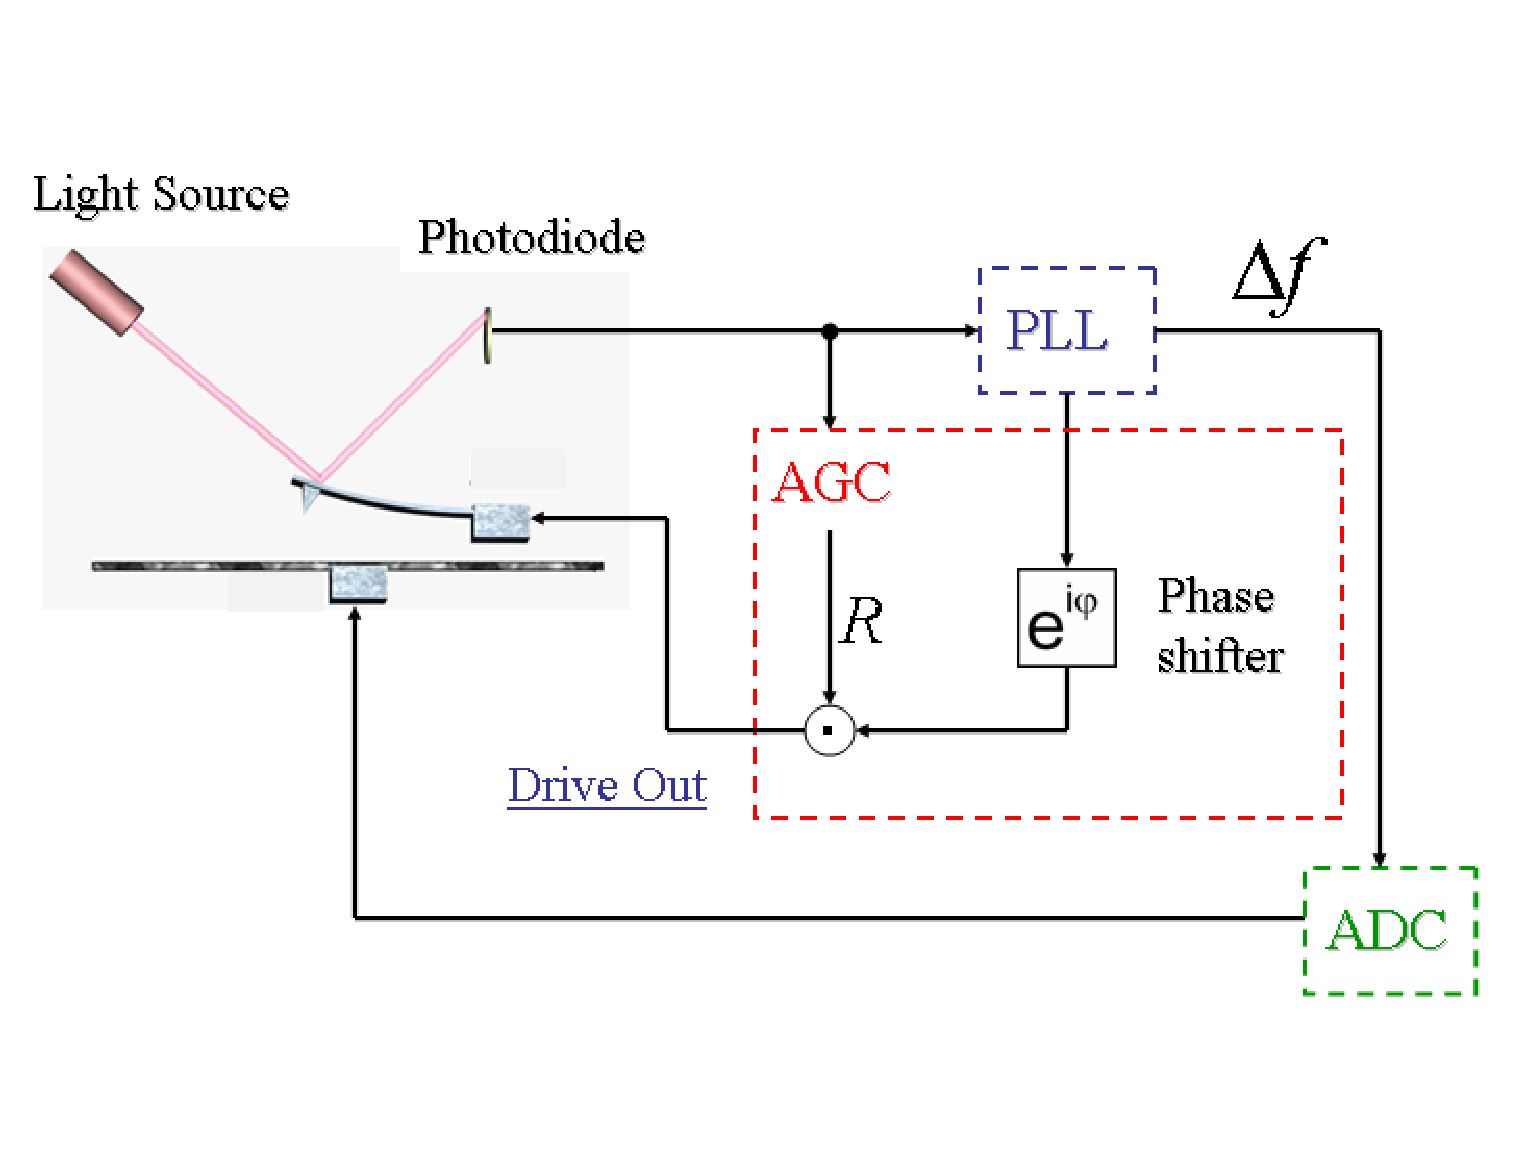
\includegraphics[%
  height=7cm,
  keepaspectratio]{pictures/fmafm.ps}\end{center}


\caption{Schematic of the FM-AFM. \label{fFMAFM}}
\end{figure}


FM-AFM involves two control loops: 

\begin{itemize}
\item The first one is supposed to maintain the cantilever oscillation amplitude
at a preset value $A_{0}$ (typically from a few nm to tens of nm).
This is achieved by an Automatic Gain Control block (AGC), which acts
on the power delivered to the cantilever excitation piezoelectric
ceramics. This power can be made proportional to the power dissipated
by the tip-surface interaction by a proper setting of the phase of
the excitation drive of the cantilever \cite{durig-pll,loppacher-phase,pfeiffer-phase}.
It is used to produce dissipation images.
\item The second one is supposed to maintain the resonance frequency shift
induced by the tip-surface interaction at a preset value $\Delta f_{c}$
(typically from a few Hz to hundreds of Hz). This is achieved by an
Automatic Distance Control block (ADC), which adjusts the tip-surface
distance $D(t)$. It is used to produce \char`\"{}topographic\char`\"{}
images. 
\end{itemize}

\subsubsection{Equation of motion of the cantilever\label{sub:Equation-of-motion}}

The dynamics of the cantilever is giverned by the following equation
of motion: 

\begin{equation}
M\ddot{z}(t)+\frac{M\omega_{0}}{Q}\dot{z}(t)+kz(t)=RA_{pll}\sin(\omega_{pll}t+\varphi)+F_{int}\left(z(t)+D(t);\dot{z}(t)\right)\label{eq:eDynamic}\end{equation}
It is solved numericacally using the velocity Verlet algorithm\cite{verlet-algo}.
In this equation $z(t)$ is the vertical displacement of the cantileved
around its mean value. The actual distance of the cantilever from
the surface plane is given by $z(t)+D(t)$ as shown in Fig. \ref{cap:tip-oscillations}.
%
\begin{figure}[!ht]
\begin{center}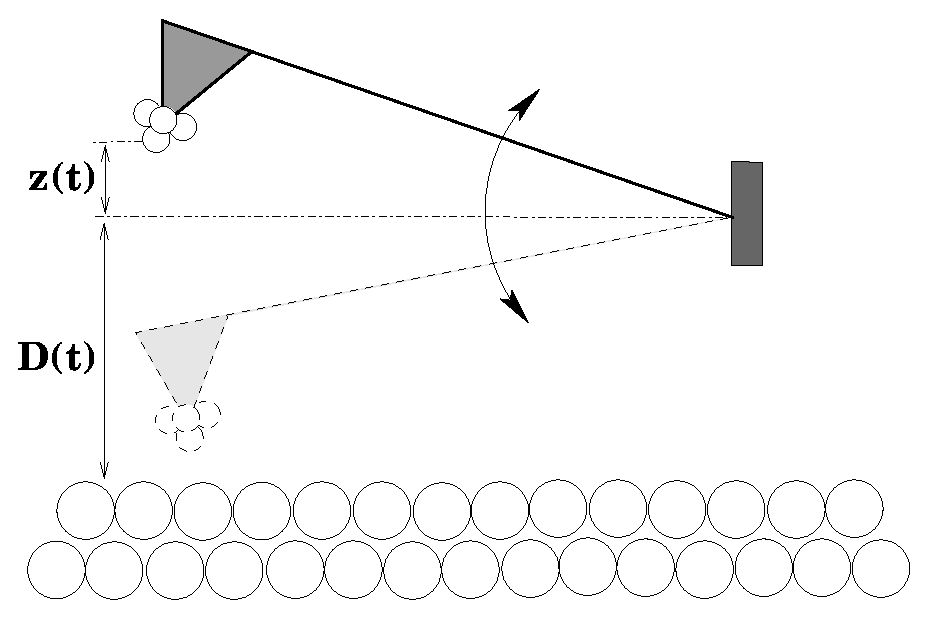
\includegraphics[%
  height=5cm]{xfig.tip.eps}\end{center}


\caption{Schematic of the oscilating cantilever system. \label{cap:tip-oscillations}}
\end{figure}


Various terms in the above equation have the following meaning:

\begin{itemize}
\item Terms in the LHS correspond to a damped harmonic oscillator: $M=k/\omega_{0}^{2}$
is the effective cantilever mass, where $k$ is cantilever stiffness
and $\omega_{0}=2\pi f_{0}$ is the resonance frequency of the free
cantilever; in addition, there is also a friction term in the LHS
containing the dimensionless quality factor $Q$; these are all intrinsic
parameters of the probe. 
\item The first term in the RHS is the excitation signal which is used to
maintain the cantilever oscillation amplitude at a preset value $A_{0}$.
The first factor in the excitation amplitude $R$ is called a damping
or dissipation term and is considered in section \ref{sub:Amplitude-regulation}
in more detail. It's just a variable gain. Note that the other part
of the signal, $A_{pll}\sin(\omega_{pll}t+\varphi)$, is produced
by the PLL as described in more detail in sections \ref{sub:Amplitude-regulation}
and \ref{sub:Frequency-demodulation}. It drives the piezo of the
cantilever.
\item $F_{int}\left(z(t)+D(t);\dot{z}(t)\right)$ corresponds to the conservative
and dissipative interactions between the tip and the surface (the
latter is not implemented presently).
\end{itemize}

\subsubsection{Amplitude regulation \label{sub:Amplitude-regulation}}

Amplitude regulation is achieved by the Automatic Gain Control (see
figure \ref{fAGC}). The modulus $A(t)$ of the cantilever oscillation
$z(t)$ is extracted by a diode followed by a first-order low-pass
filter, modelized by:

\begin{equation}
A(t)=\frac{\pi}{2\tau_{D}}e^{-t/\tau_{D}}\int_{0}^{t}\left|z(t^{\prime})\right|e^{t/\tau_{D}}\textrm{d}t^{\prime}\label{eq:ePeakDetection}\end{equation}
with $\tau_{D}$ being the time constant of the envelope detection. 

%
\begin{figure}[!ht]
\begin{center}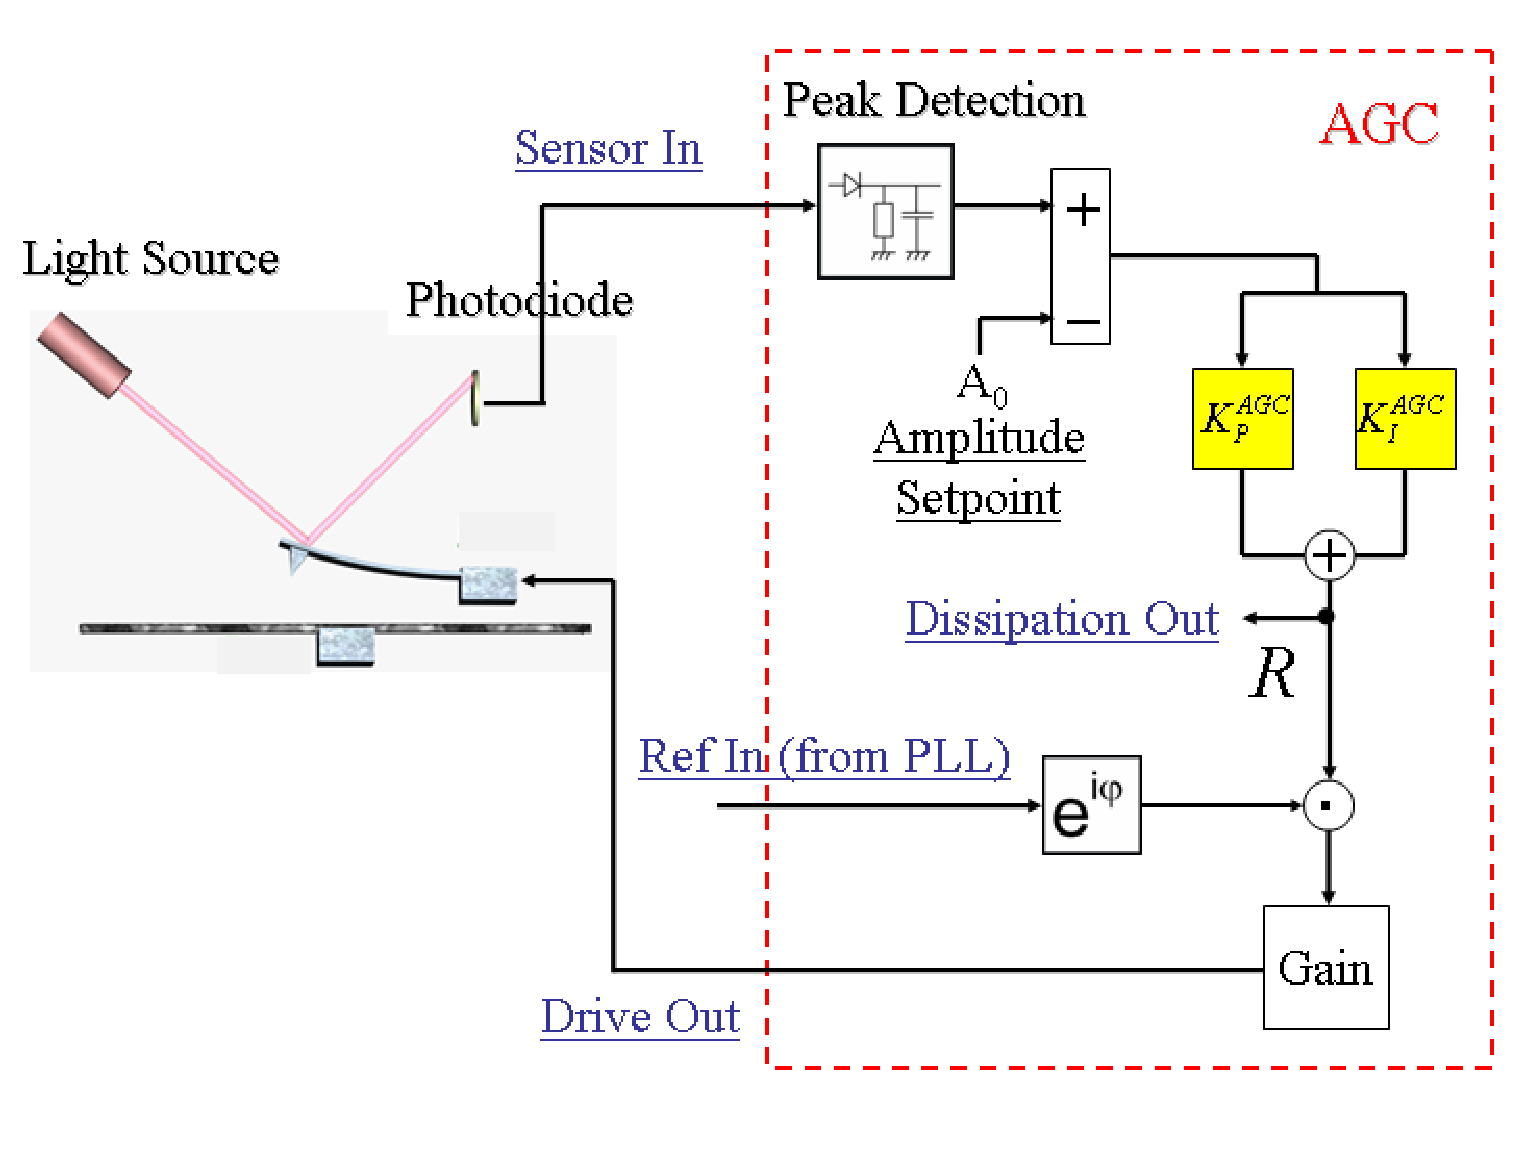
\includegraphics[%
  height=7cm,
  keepaspectratio]{pictures/agc.ps}\end{center}


\caption{Automatic Gain Control. \label{fAGC}}
\end{figure}


$A(t)$ is then compared to the amplitude setpoint $A_{0}$. The error
signal $A(t)-A_{0}$, after being fed into a PI (Proportional-Integral)
system \cite{etique-automatique,silva-PI,Wang-PI}, is used to change
the variable gain $R(t)$. Both the Proportional gain $K_{P}^{AGC}$
(controlling the {}``stiffness'' of the AGC loop) and the Integration
gain $K_{I}^{AGC}$ (controlling the {}``viscosity'' of the AGC
loop) can be set by the user. One obtains the dynamic gain $R(t)$:

\begin{equation}
R(t)=K_{P}^{AGC}\left[A(t)-A_{0}\right]+K_{I}^{AGC}\int_{-\infty}^{t}\left[A(t')-A_{0}\right]\; dt'\label{eq:eAGC}\end{equation}


Without tip-surface interaction, $R(D\rightarrow\infty)=\frac{k_{c}\, A_{0}}{Q_{c}}$
with $A_{pll}=1.$


\subsubsection{Frequency demodulation and cantilever excitation\label{sub:Frequency-demodulation}}

%
\begin{figure}[!ht]
\begin{center}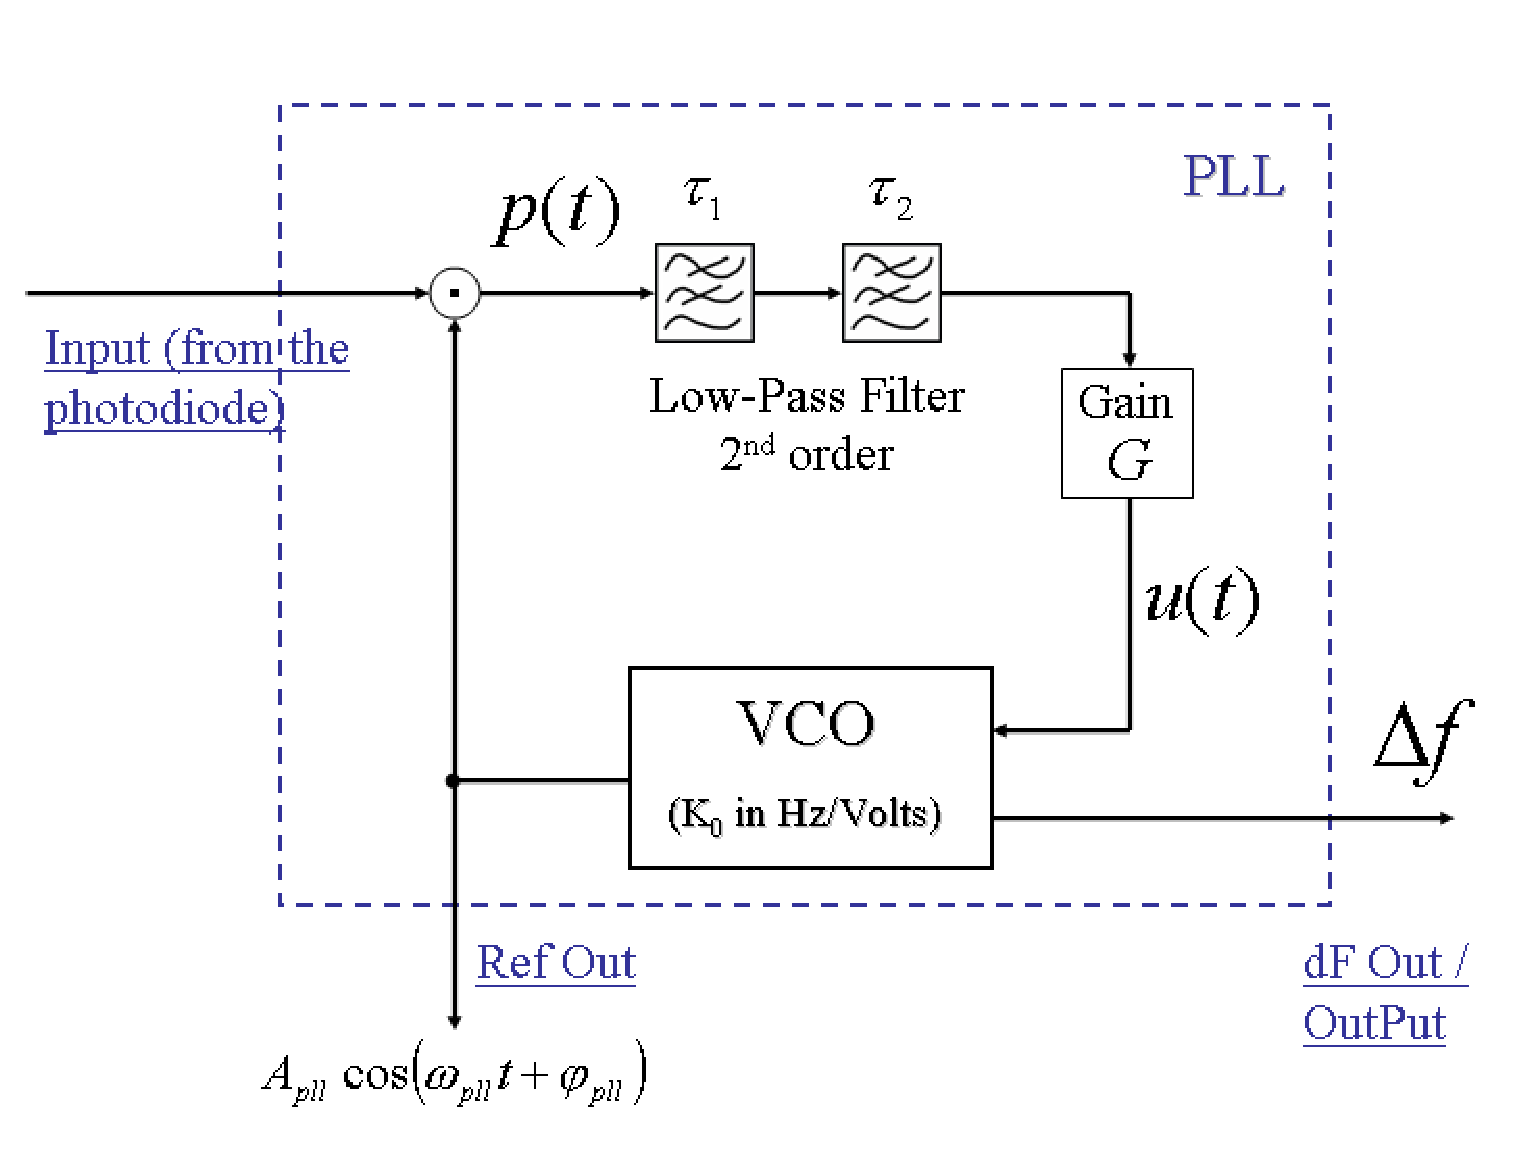
\includegraphics[%
  height=7cm,
  keepaspectratio]{pictures/pll.ps}\end{center}


\caption{Phase Locked Loop\label{fPLL}}
\end{figure}


Far from any tip-surface interaction, the pulsation $\omega_{pll}(t)$
of the PLL (see figure \ref{fPLL}) reference signal is set by the
user to the free frequency of the cantilever such as $\omega_{pll}(t)=\omega_{0}$.
The VCO (Voltage Controlled Oscillator), inside the PLL, produces
this reference signal by the integration of the input voltage $u(t)$: 

\begin{equation}
\omega_{pll}(t)\, t=\omega_{0}\, t+\int_{-\infty}^{t}\Delta\omega(t')\; dt'=\omega_{0}\, t+K_{0}\int_{-\infty}^{t}u(t')\; dt'\label{eq:eVCO}\end{equation}


where $K_{0}$ (in Hz) is the conversion factor (voltage to frequency)
of the VCO \cite{loppacherPLL}.

The signal $u(t)$ which is proportional to the detuning, $\Delta\omega(t)=\omega(t)-\omega_{0}$,
of the cantilever frequency, is obtained by low-pass filtering the
product $p(t)$ of the reference signal by the cantilever signal $z(t)$
coming from the photodiode. Hence:

\begin{center}\begin{equation}
p(t)=z(t)\, A_{pll}\,\cos(\omega_{pll}(t)\, t+\varphi_{pll})\label{eq:qProduct}\end{equation}
\end{center}

In first approximation, if we consider $z(t)=A(t)\:\sin(\omega(t)\, t+\varphi)$,
one obtains:

\begin{equation}
p(t)=\frac{A_{limited}\, A_{pll}}{2}\,\left[\sin((\omega(t)-\omega_{pll}(t))\, t+(\varphi-\varphi_{pll}))+\sin((\omega(t)+\omega_{pll}(t))\, t+(\varphi+\varphi_{pll}))\right]\label{eq:eProduct2}\end{equation}


with a limiter circuit, at the input of the PLL, that limits the signal
amplitude $A(t)$ to a constant level $A_{limited}$. 

This signal $p(t)$ then goes through a second order low-pass filter
defined by two time constants $\tau_{1}$ and $\tau_{2}$:

\begin{equation}
p_{1}(t)=\left[\frac{1}{\tau_{1}}\int^{t}p(t')\exp\left(\frac{t'}{\tau_{1}}\right)\; dt'\right]\exp\left(\frac{-t}{\tau_{1}}\right)\label{eq:eLowPass1}\end{equation}


\begin{equation}
u(t)=G\,\left[\frac{1}{\tau_{2}}\int^{t}p_{1}(t')\exp\left(\frac{t'}{\tau_{2}}\right)\; dt'\right]\exp\left(\frac{-t}{\tau_{2}}\right)\label{eq:eLowPass2}\end{equation}


Thanks to this low-pass filter, the low frequency part, $\omega(t)-\omega_{pll}(t)$,
of the signal $p(t)$ is extracted. The parameter $G$ allows to adjust
the loop gain of the PLL in order to find the good stability-precision
compromise \cite{loppacher-dissertation}. Hence:

\begin{equation}
u(t)=G\,\frac{A_{limited}\, A_{pll}}{2}\,\sin((\omega(t)-\omega_{pll}(t))\, t+(\varphi-\varphi_{pll}))\label{eq:eU}\end{equation}


When $\omega_{pll}(t)=\omega(t)$, the PLL is locked on the cantilever
frequency. So, one can write, in the case of small changes $\Delta\varphi=\varphi-\varphi_{pll}$:

\begin{equation}
u(t)\simeq G\,\frac{A_{limited}\, A_{pll}}{2}\,\Delta\varphi\label{eq:eUphy}\end{equation}


giving the frequency detuning $\Delta\omega(t)=K_{0}\, u(t)$.


\subsubsection{Distance regulation\label{sub:Distance-regulation}}

%
\begin{figure}[!ht]
\begin{center}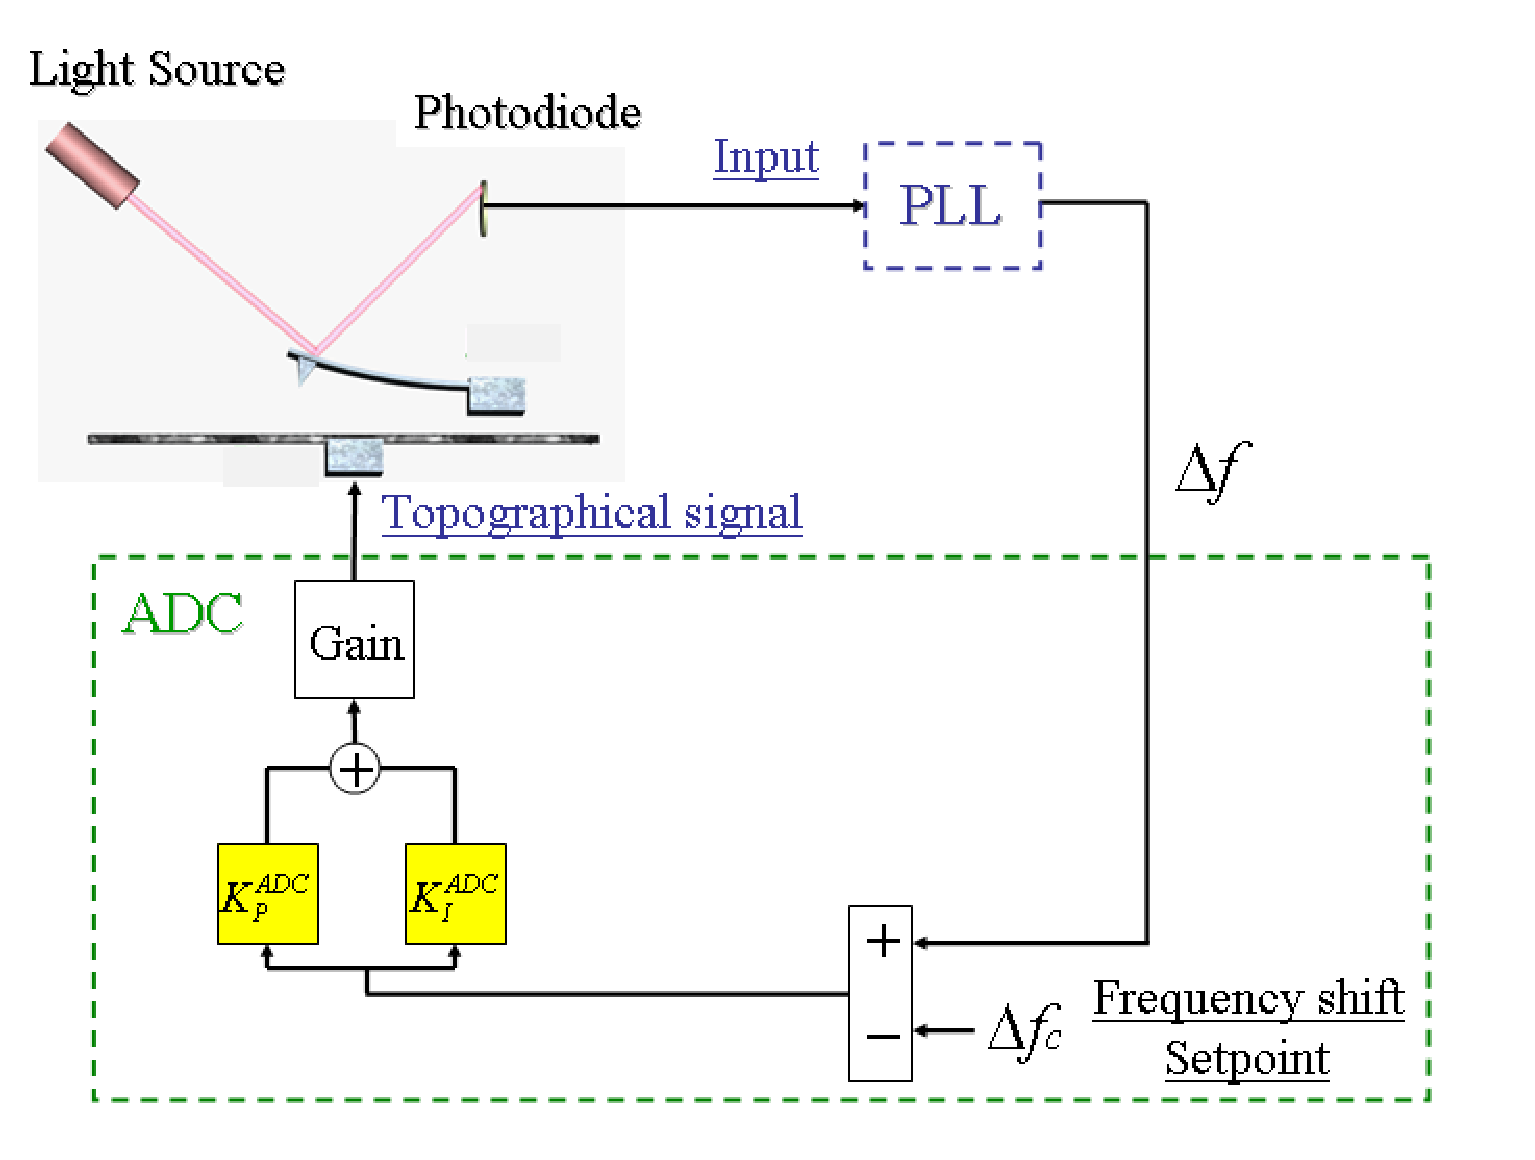
\includegraphics[%
  height=7cm,
  keepaspectratio]{pictures/adc.ps}\end{center}


\caption{Automatic Distance Control. \label{fADC}}
\end{figure}


The $\Delta f(t)=\frac{\Delta\omega(t)}{2\pi}$ signal coming from
the frequency demodulator (see figure \ref{fPLL}) is used to regulate
the distance $D(t)$ between the cantilever and the surface in order
to satisfy the frequency setpoint $\Delta f_{c}$ (see figure \ref{fADC})
defined by the user \cite{albrecht-fmdemodul,durig-fmdemodul}. Following
this rule, one gets the following expression:

\begin{equation}
D(t)=D_{1}+K_{P}^{ADC}\left[\Delta f(t)-\Delta f_{c}\right]+K_{I}^{ADC}\int_{-\infty}^{t}\left[\Delta f(t')-\Delta f_{c}\right]\; dt'\label{eq:eADC}\end{equation}


where we find, like in the AGC (see equation \ref{eq:eAGC}), a PI
(Proportional-Integral) system with gains $K_{P}^{ADC}$ and $K_{I}^{ADC}$
defined by the user. $D_{1}$ is an ajustable offset in distance.


\subsection{Influence of experimental noises on AFM images}

Another useful application of the virtual AFM is the realistic evaluation
of the limitations imposed by the noise generated by the components
of the system. Sources of noise in beam deflection AFM have been discussed
in \cite{sarid}. The major ones are \cite{yaralioglu-allnoises}:

The thermal noise of the cantilever \cite{cleland-cantilevernoise,albrecht-fmdemodul},
whose power spectral density reads: \begin{equation}
S_{F}(f)=\frac{4\, k_{B}\, T\, k}{2\pi\, f_{0}\, Q}\qquad\textrm{in }N^{2}.Hz^{-1}\label{eForceNoise}\end{equation}
 with the temperature $T$, the Boltzmann constant $k_{B}$. In virtual
AFM, this noise is implemented at left in equation \ref{eq:eDynamic}
as a noise force.

The amplitude shot noise \cite{bacon-shotnoise,yaralioglu-allnoises}
of one photodiode quadrant detector: \begin{equation}
S_{A}^{shot-noise}(f)=2\, q_{e}\, V_{ph}\, R_{trans}\, G_{opt}^{2}\qquad\textrm{in }m^{2}.Hz^{-1}\label{eAmplitudeShotNoise}\end{equation}


with the elementary charge $q_{e}$, the photodiode voltage $V_{ph}$
($1\, Volt$ in our experimental conditions), the transimpedance resistor
$R_{trans}$ ($500\, k\Omega$ \cite{Omicron}). $G_{opt}$ is a factor
to convert the cantilever oscillation in volts coming from the photodiode
in nanometers. It depends of the geometrical design of the optical
detection but also of the kind of light source used (Laser, LED, ...).
In our case, we measured $G_{opt}=400\, nm.V^{-1}$. 

Finally, the Johnson noise of the resistor of the current-voltage
converter that monitors the photodiodes: \begin{equation}
S_{A}^{Johnson}(f)=4\, k_{B}\, T\, R_{trans}\, G_{opt}^{2}\qquad\textrm{in }m^{2}.Hz^{-1}\label{eAmplitudeJohnsonNoise}\end{equation}


The amplitude shot noise and Johnson noise are both used as amplitude
noises inside $z(t)$ the vertical displacement of the cantilever
coming from the photodiode signal.


\subsection{How one can find parameters of the virtual AFM}

The aim of the virtual machine is to mimic the dynamic of a true experimental
AFM system. In this subsection we shall briefly describe a response
of the whole machine (Omicron RT-AFM with an easyPLL Nanosurf Demodulator)
on a square periodic offset added to the distance signal $D(t)$.
This is an example of how one can experimentally find the correct
parameters needed to run the virtual AFM machine.

Fig. \ref{fCompareExpNum} (a) shows the frequency response to a periodic
square excitation added to the surface-tip distance $D$ while the
microscope was in operation above a ${\rm MoS_{2}}$ substrate covered
by silver clusters. This measurement was performed for two different
settings of the ADC feedback loop. A loop gain of 2\% (slow response)
corresponds to the typical value for normal imaging while a loop gain
of 20\% (fast response) is only used when approaching the surface
at the beginning of the experiment. The asymmetry of the response
between a positive and negative $\Delta f$ (the positive peak is
smaller and wider than the negative one) is a consequence of the increase
of the absolute value of the slope of the van der Waals interaction
when the tip approaches the surface.

Fig. \ref{fCompareExpNum} (b) shows the response calculated with
the virtual AFM modelling the tip by a sphere of the radius 20 nm
and taking into account only the van der Waals interaction between
tyhe tip and sample, with a Hamaker constant of 1 eV. The experimental
behaviour can be well reproduced by choosing the parameters $K_{P}^{ADC}$
and $K_{I}^{ADC}$ \cite{Wang-PI}. The shape of the peaks is qualitatively
correct while the time constants, ranging from a few milliseconds
at 20\% to a few tens of milliseconds at 2\%, are of the same order
of magnitude as in the experiment. 

\begin{center}%
\begin{figure}[!ht]
\begin{center}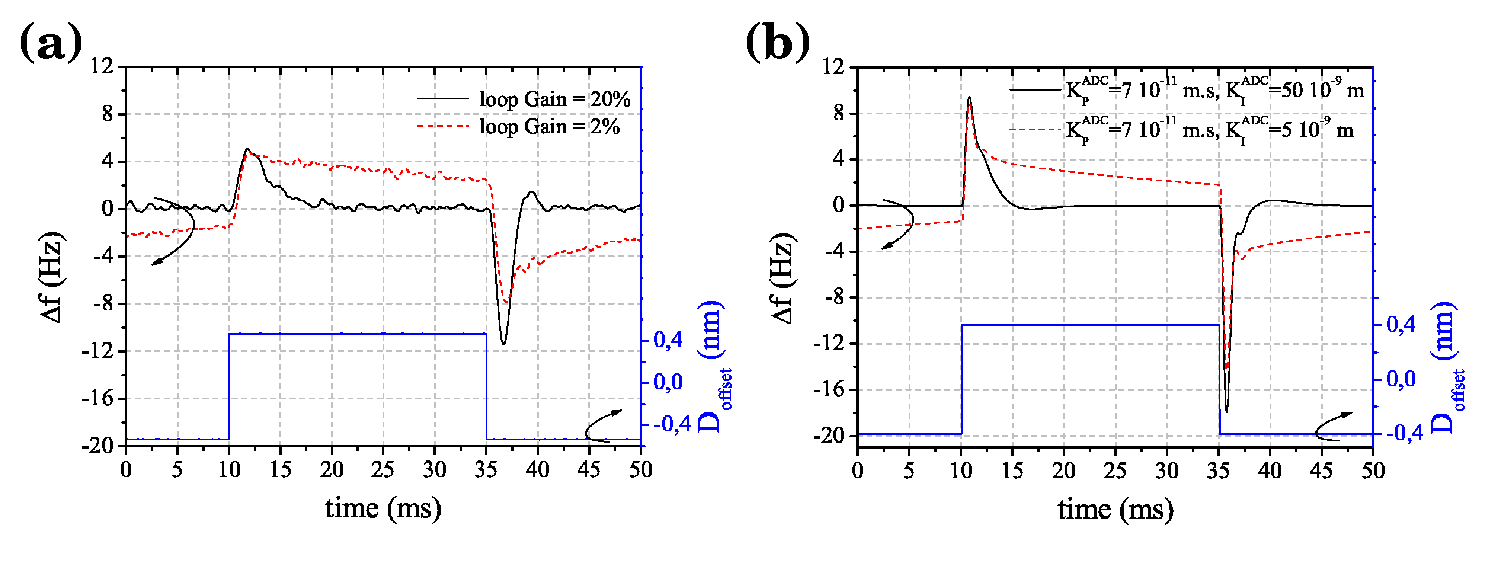
\includegraphics[%
  height=6cm]{pictures/xfig.offset.eps}\end{center}


\caption{Experimental (a) and calculated (b) response of the ADC. Electrostatic
forces have been compensated following Ref. \cite{guggisberg-electrostatic}.
\label{fCompareExpNum}}
\end{figure}
\end{center}


\newpage
\part{Installation}


\section{How to compile the code}

The code should be in the form of a gzipped tarball, such as \texttt{scifi\_3.51.tgz}.
Assuming this, then type:
\bigskip{}

\texttt{tar -zxvf scifi\_3.51.tgz}
\bigskip{}

\noindent this will extract all the necessary files, including directories
\texttt{SHELLM} (the main code including the vAFM part) and \texttt{IMAGE}
(the image part of the code), a directory \texttt{examples} containing
three example input files and the corresponding output files. 

To compile the program, a \texttt{Makefile} in either of the directories
\texttt{SHELLM} and \texttt{IMAGE,} should be edited to include the
command of your Fortran 77 or Fortran 90 compiler (g77 is the default),
along with any compiler options (-o (optimised) is default). 

The code can be compiled into either a serial execultable or a MPICH
parallel version, via the \texttt{cpp} precompiler. To compile a parallel
version, the \texttt{MPIFLAG = -DMPI} must be added to the \texttt{Makefile},
as well as the MPICH flags to your compiler and the path of your \texttt{mpich.h}
header file. 

To compile the code, type \texttt{}
\smallskip{}

\texttt{make} 
\smallskip{}

\noindent in either of the two directories; this will produce the
executables \texttt{shellm} and \texttt{image}, respectively. Make
sure that you have access to both executables, i.e. that the directories
are included in the \texttt{\$path} variable. 

You can now run the code (see below how). Make sure that you can reproduce
the output from the the example inputs provided in the \texttt{examples}
directory (section \ref{Sec::Example-Inputs}).


\section{parameter file}

The file \texttt{param.inc} in the main directory contains all the
matrix sizes for the calculation. This file must be edited before
compilation if changes are needed. Below is an example:
\bigskip{}

\texttt{\footnotesize ~ ~~ ~implicit real{*}8 (a-h,o-z) }{\footnotesize \par}

\texttt{\footnotesize c............. parameters: }{\footnotesize \par}

\texttt{\footnotesize c N0KD - max number of species }{\footnotesize \par}

\texttt{\footnotesize c N0LT - max number of atoms }{\footnotesize \par}

\texttt{\footnotesize c N0CH - max number of all charges (cores+shells) }{\footnotesize \par}

\texttt{\footnotesize c N0PAR - number of exp/power terms in the short-range
interaction }{\footnotesize \par}

\texttt{\footnotesize c N0FR=max\_free - max number of degrees of
freedom for optimisation }{\footnotesize \par}

\texttt{\footnotesize c isaved\_step - the MD restart saving interval }{\footnotesize \par}

\texttt{\footnotesize c max\_proc - maximum number of processors }{\footnotesize \par}

\texttt{\footnotesize c N0BD - maximum number of covailent bonds per
atom}{\footnotesize \par}
\bigskip{}

\texttt{\footnotesize ~ ~~ ~parameter ( N0PAR=5,N0KD=10, N0LT=4500,
N0CH=2{*}N0LT ) }{\footnotesize \par}

\texttt{\footnotesize ~ ~~ ~parameter ( N0KD1=N0KD{*}(N0KD+1)/2
) }{\footnotesize \par}

\texttt{\footnotesize ~ ~~ ~parameter ( N0FR=6300 , max\_free=N0FR) }{\footnotesize \par}

\texttt{\footnotesize c BFGS\_st\_desc\_max - max number of times
BFGS can run steepest descent }{\footnotesize \par}

\texttt{\footnotesize c in a row. This prevents the code to get stuck
in this. }{\footnotesize \par}

\texttt{\footnotesize ~ ~~ ~parameter ( iBFGS\_st\_desc\_max=1) }{\footnotesize \par}

\texttt{\footnotesize ~ ~~ ~parameter (isaved\_rst = 100) }{\footnotesize \par}

\texttt{\footnotesize ~ ~~ ~parameter ( N0BD = 6) }{\footnotesize \par}

\texttt{\footnotesize ~ ~~ ~parameter ( max\_proc = 100 ) }{\footnotesize \par}

\texttt{\footnotesize c N0CNSTR - max number of constraints }{\footnotesize \par}

\texttt{\footnotesize c NinvAt0 - max number of atoms participating
in every constarint parameter (N0CNSTR=10,NinvAt0=10)}{\footnotesize \par}

~

\noindent These are the default values, but they can be reduced to
reduce memory demands or increased for bigger systems. The most crucial
parameter is \texttt{N0LT} which controls the maximum number of charges
(\texttt{N0CH = 2{*}N0LT}) in the system, if this is changed then
\texttt{N0FR}, the maximum degrees of freedom, should be changed correspondingly.


\section{virtual\_param.inc file\label{sub:virtual_param.inc-file}}

The file \texttt{virtual\_param.inc} contains all the matrix sizes
for the calculation. This file must be edited and a compilation performed
if changes are needed. Below is an example:
\bigskip{}

\texttt{\footnotesize parameter (pi=3.141592653589793d0, twopi=2.d0{*}pi)}{\footnotesize \par}

\texttt{\footnotesize c........ max number of steps/stages }{\footnotesize \par}

\texttt{\footnotesize parameter (N\_of\_stages\_max=99)}{\footnotesize \par}

\texttt{\footnotesize c......... scans: max number of scans allowed }{\footnotesize \par}

\texttt{\footnotesize parameter (N\_of\_scans\_max=5)}{\footnotesize \par}

\texttt{\footnotesize c......... units: distance, force double precision
m\_A,N\_eVpA,J\_eV}{\footnotesize \par}

\texttt{\footnotesize parameter (m\_A=1.0d10,N\_eVpA=6.2415d8,J\_eV=6.2415d18)}{\footnotesize \par}

\texttt{\footnotesize c......... threshold for the distance }{\footnotesize \par}

\texttt{\footnotesize parameter (threshold=1.0d-10) }{\footnotesize \par}

\smallskip{}
\begin{flushleft}The most important parameters are: \end{flushleft}

\begin{itemize}
\item \texttt{N\_of\_stages\_max} - maximum number of elementary stages
for the whole run
\item \texttt{N\_of\_scans\_max} - maximum number of scans allowed during
a single run
\end{itemize}

\section{How to run the code}

The code is run with a command line like this:

\texttt{scifi name option}
\bigskip{}

\noindent where \texttt{name} is the job identifier. 


\newpage
\part{Input}


\section{General}

\noindent The code reads in a single unformatted input file which
can be in one of two forms: either an initial file (\texttt{name.INN})
or a restart file (\texttt{name.RST}). The only difference is that
a restart file has been produced by the code itself and normally contains
relaxed positions of atoms and shell-polarization. A restart file
will automatically be produced after every run of the code, regardless
of the options selected. 

The code will use an initial (\texttt{.INN}) file of the appropriate
name if no \texttt{option} is given. If the keyword 'restart' is given
as an option then the program will open the restart file of the appropriate
name as input. The code will also produce an input file \texttt{input.img}
if the \texttt{.<IMAGE>} box is present. This contains all atomic
positions (excluding \textbf{frozen-tip}), charges and general information
about the system relevant to the image calculation, and can be ignored
except for debugging purposes. The image part of the code runs independently
of the main code, but is called automatically without requiring user
intervention.

The input file itself is separated into specific boxes for each category
of input parameters. Each box begins with the keyword name of the
box in the format \emph{.<keyword>} and then the appropriate keywords
and parameters for that box are listed. Keywords must be placed in
the input box they are classed in, they will be ignored in other boxes.
Some keywords require another controlling word or parameter value,
whereas others are activated by just being present. After the example
file, each box and its keywords are explained, along with possible
parameters which can be used.

Comments can be entered into the input file by placing \#\# before
the line. Empty lines will be ignored. There is no specific order
required for the boxes in the input file, but there is some order
needed for specific keywords within the boxes. These position dependent
keywords will be highlighted below.

Boxes described in Section \ref{sec:SciFi-input} correspond to the
SciFi part of the code. If an error is generated when reading those
boxes (in particular, if some or all boxes are missing), then the
SciFi part is switched off. Next, an vAFM input is read in. If there
is no error, the vAFM part of the code is working relying on an existing
force field. Otherwise, the code stops with an error message. Conversely,
if there is only an error in the vAFM part, then the code works as
a SciFi code. The vAFM input part is described separately in Section 


\section{SciFi input\label{sec:SciFi-input}}


\subsection{Example Input File}

This input file contains a system where the tip consists of only one
atom at the end of a conducting sphere interacting with a small defected
cluster on top of a conducting substrate. 

\texttt{\footnotesize ~}{\footnotesize \par}

\texttt{\footnotesize .<Toleranc>}{\footnotesize \par}

\texttt{\footnotesize do\_md}{\footnotesize \par}

\texttt{\footnotesize printing tiny}{\footnotesize \par}

\texttt{\footnotesize shells frozen}{\footnotesize \par}

\texttt{\footnotesize xyz write}{\footnotesize \par}

\texttt{\footnotesize \#\#g98-file write}{\footnotesize \par}

\texttt{\footnotesize max\_opt~~~ 1}{\footnotesize \par}

\texttt{\footnotesize optim bfgs}{\footnotesize \par}

\texttt{\footnotesize en\_tol 0.150000E-05}{\footnotesize \par}

\texttt{\footnotesize es\_tol 0.500000E-01}{\footnotesize \par}

\texttt{\footnotesize frc\_tol 0.100000E-01}{\footnotesize \par}

\texttt{\footnotesize crd\_tol 0.500000E-01}{\footnotesize \par}

\texttt{\footnotesize \#\#test 0.0001}{\footnotesize \par}

\texttt{\footnotesize .<End>}{\footnotesize \par}

~

\texttt{\footnotesize .<MDcontrol> }{\footnotesize \par}

\texttt{\footnotesize numsteps 2000 }{\footnotesize \par}

\texttt{\footnotesize tstep 0.00001 }{\footnotesize \par}

\texttt{\footnotesize dtemp 330.000 }{\footnotesize \par}

\texttt{\footnotesize algorithm nve}{\footnotesize \par}

\texttt{\footnotesize shells dynamic }{\footnotesize \par}

\texttt{\footnotesize tau 0.2000 }{\footnotesize \par}

\texttt{\footnotesize statistics 1 }{\footnotesize \par}

\texttt{\footnotesize trajectory 20 }{\footnotesize \par}

\texttt{\footnotesize traj\_fmt 1 }{\footnotesize \par}

\texttt{\footnotesize vel\_key 0 }{\footnotesize \par}

\texttt{\footnotesize .<End>}{\footnotesize \par}

\texttt{\footnotesize ~}{\footnotesize \par}

\texttt{\footnotesize .<ShellPar>}{\footnotesize \par}

\texttt{\footnotesize ~O~ 0.400000E-01 -.204000E+01 0.143000E+02}{\footnotesize \par}

\texttt{\footnotesize Mg~ 0.200000E+01 0.000000E+00 0.000000E+00}{\footnotesize \par}

\texttt{\footnotesize Cr~ 0.300000E+01 0.000000E+00 0.000000E+00}{\footnotesize \par}

\texttt{\footnotesize .<End>}{\footnotesize \par}

\texttt{\footnotesize ~}{\footnotesize \par}

\texttt{\footnotesize .<Coord>}{\footnotesize \par}

\texttt{\footnotesize \#\#move 1.0 1.0 1.0}{\footnotesize \par}

\texttt{\footnotesize \#\#rotate 90.0 90.0 90.0}{\footnotesize \par}

\texttt{\footnotesize \#\#centre 5.0 5.0 5.0}{\footnotesize \par}

\texttt{\footnotesize \#\#scan 0.2}{\footnotesize \par}

\texttt{\footnotesize ~}{\footnotesize \par}

\texttt{\footnotesize tip-atoms}{\footnotesize \par}

\texttt{\footnotesize Cr~~~ 0.00000~~~ 0.00000~~~ 5.50000~~~~~
1 1 1}{\footnotesize \par}

\texttt{\footnotesize cluster-atoms }{\footnotesize \par}

\texttt{\footnotesize Cr~~~ 0.00000~~~ 0.00000~~~ 0.00000~~~~~
1 1 1}{\footnotesize \par}

\texttt{\footnotesize O~~~ -2.12200~~~ 0.00000~~~ 0.00000~~~~~
1 1 1}{\footnotesize \par}

\texttt{\footnotesize O~~~~ 0.00000~~ -2.12200~~~ 0.00000~~~~~
1 1 1}{\footnotesize \par}

\texttt{\footnotesize O~~~~ 0.00000~~~ 0.00000~~ -2.12200~~~~~
1 1 1}{\footnotesize \par}

\texttt{\footnotesize O~~~~ 0.00000~~~ 2.12200~~~ 0.00000~~~~~
1 1 1}{\footnotesize \par}

\texttt{\footnotesize O~~~~ 2.12200~~~ 0.00000~~~ 0.00000~~~~~
1 1 1}{\footnotesize \par}

\texttt{\footnotesize Mg~~ -2.12200~~ -2.12200~~~ 0.00000~~~~~
1 1 1}{\footnotesize \par}

\texttt{\footnotesize Mg~~ -2.12200~~~ 2.12200~~~ 0.00000~~~~~
1 1 1}{\footnotesize \par}

\texttt{\footnotesize Mg~~~ 2.12200~~ -2.12200~~~ 0.00000~~~~~
1 1 1}{\footnotesize \par}

\texttt{\footnotesize Mg~~~ 2.12200~~~ 2.12200~~~ 0.00000~~~~~
1 1 1}{\footnotesize \par}

\texttt{\footnotesize Mg~~ -4.24400~~~ 0.00000~~~ 0.00000~~~~~
1 1 1}{\footnotesize \par}

\texttt{\footnotesize Mg~~~ 0.00000~~ -4.24400~~~ 0.00000~~~~~
1 1 1}{\footnotesize \par}

\texttt{\footnotesize Mg~~~ 0.00000~~~ 4.24400~~~ 0.00000~~~~~
1 1 1}{\footnotesize \par}

\texttt{\footnotesize Mg~~~ 4.24400~~~ 0.00000~~~ 0.00000~~~~~
1 1 1}{\footnotesize \par}

\texttt{\footnotesize Mg~~~ 0.00000~~ -2.12200~~ -2.12200~~~~~
1 1 1}{\footnotesize \par}

\texttt{\footnotesize Mg~~~ 0.00000~~~ 2.12200~~ -2.12200~~~~~
1 1 1}{\footnotesize \par}

\texttt{\footnotesize Mg~~ -2.12200~~~ 0.00000~~ -2.12200~~~~~
1 1 1}{\footnotesize \par}

\texttt{\footnotesize Mg~~~ 2.12200~~~ 0.00000~~ -2.12200~~~~~
1 1 1}{\footnotesize \par}

\texttt{\footnotesize Mg~~~ 0.00000~~~ 0.00000~~ -4.24400~~~~~
1 1 1}{\footnotesize \par}

\texttt{\footnotesize O~~~ -2.12200~~ -2.12200~~ -2.12200~~~~~
1 1 0}{\footnotesize \par}

\texttt{\footnotesize O~~~ -2.12200~~~ 2.12200~~ -2.12200~~~~~
1 1 0}{\footnotesize \par}

\texttt{\footnotesize O~~~~ 2.12200~~ -2.12200~~ -2.12200~~~~~
1 1 0}{\footnotesize \par}

\texttt{\footnotesize O~~~~ 2.12200~~~ 2.12200~~ -2.12200~~~~~
1 1 0}{\footnotesize \par}

\texttt{\footnotesize O~~~ -4.24400~~ -2.12200~~~ 0.00000~~~~~
1 1 0}{\footnotesize \par}

\texttt{\footnotesize O~~~ -4.24400~~~ 0.00000~~ -2.12200~~~~~
1 1 0}{\footnotesize \par}

\texttt{\footnotesize O~~~ -4.24400~~~ 2.12200~~~ 0.00000~~~~~
0 0 0}{\footnotesize \par}

\texttt{\footnotesize O~~~ -2.12200~~ -4.24400~~~ 0.00000~~~~~
0 0 0}{\footnotesize \par}

\texttt{\footnotesize O~~~ -2.12200~~~ 0.00000~~ -4.24400~~~~~
0 0 0}{\footnotesize \par}

\texttt{\footnotesize O~~~ -2.12200~~~ 4.24400~~~ 0.00000~~~~~
0 0 0}{\footnotesize \par}

\texttt{\footnotesize O~~~~ 0.00000~~ -4.24400~~ -2.12200~~~~~
0 0 0}{\footnotesize \par}

\texttt{\footnotesize .<End>}{\footnotesize \par}

\texttt{\footnotesize ~}{\footnotesize \par}

\texttt{\footnotesize .<BondToleranc> }{\footnotesize \par}

\texttt{\footnotesize O O 0.000000000000000 0.000000000000000 }{\footnotesize \par}

\texttt{\footnotesize Mg O 0.000000000000000 0.000000000000000 }{\footnotesize \par}

\texttt{\footnotesize Mg Mg 0.000000000000000 0.000000000000000}{\footnotesize \par}

\texttt{\footnotesize Cr O 0.000000000000000 0.000000000000000 }{\footnotesize \par}

\texttt{\footnotesize Mg Cr 0.000000000000000 0.000000000000000 }{\footnotesize \par}

\texttt{\footnotesize Cr Cr 0.000000000000000 0.000000000000000}{\footnotesize \par}

\texttt{\footnotesize .<End>}{\footnotesize \par}

\texttt{\footnotesize ~}{\footnotesize \par}

\texttt{\footnotesize .<PairPotenc>}{\footnotesize \par}

\texttt{\footnotesize cutoff}{\footnotesize \par}

\texttt{\footnotesize ~O~~ O~ 0.600000E+01}{\footnotesize \par}

\texttt{\footnotesize ~~~~ exp~ 1}{\footnotesize \par}

\texttt{\footnotesize ~~ 9547.90000000000~~~~~~ 0.219160000000000~~~~ }{\footnotesize \par}

\texttt{\footnotesize ~~~~ pow~ 1}{\footnotesize \par}

\texttt{\footnotesize ~ -32.8000000000000~~~~~~~ 6.00000000000000~~~~ }{\footnotesize \par}

\texttt{\footnotesize Mg~~ O~ 0.600000E+01}{\footnotesize \par}

\texttt{\footnotesize ~~~~ exp~ 1}{\footnotesize \par}

\texttt{\footnotesize ~~ 1284.38000000000~~~~~~ 0.299690000000000~~~~ }{\footnotesize \par}

\texttt{\footnotesize ~~~~ pow~ 0}{\footnotesize \par}

\texttt{\footnotesize Mg~ Mg~ 0.100000E+00}{\footnotesize \par}

\texttt{\footnotesize ~~~~ exp~ 0}{\footnotesize \par}

\texttt{\footnotesize ~~~~ pow~ 0}{\footnotesize \par}

\texttt{\footnotesize Cr~~ O~ 0.600000E+01}{\footnotesize \par}

\texttt{\footnotesize ~~~~ exp~ 1}{\footnotesize \par}

\texttt{\footnotesize ~~ 1284.38000000000~~~~~~ 0.299690000000000~~~~ }{\footnotesize \par}

\texttt{\footnotesize ~~~~ pow~ 0}{\footnotesize \par}

\texttt{\footnotesize Cr~ Mg~ 0.100000E+00}{\footnotesize \par}

\texttt{\footnotesize ~~~~ exp~ 0}{\footnotesize \par}

\texttt{\footnotesize ~~~~ pow~ 0}{\footnotesize \par}

\texttt{\footnotesize Cr~ Cr~ 0.100000E+00}{\footnotesize \par}

\texttt{\footnotesize ~~~~ exp~ 0}{\footnotesize \par}

\texttt{\footnotesize ~~~~ pow~ 0}{\footnotesize \par}

\texttt{\footnotesize .<End>}{\footnotesize \par}

\texttt{\footnotesize ~}{\footnotesize \par}

\texttt{\footnotesize ~}{\footnotesize \par}

\texttt{\footnotesize .<Image>}{\footnotesize \par}

\texttt{\footnotesize plane}{\footnotesize \par}

\texttt{\footnotesize sphere}{\footnotesize \par}

\texttt{\footnotesize decay}{\footnotesize \par}

\texttt{\footnotesize qwrite}{\footnotesize \par}

\texttt{\footnotesize printing tiny}{\footnotesize \par}

\texttt{\footnotesize precis~~~~ 15}{\footnotesize \par}

\texttt{\footnotesize Z\_plane -.110000E+02}{\footnotesize \par}

\texttt{\footnotesize bottom\_sph 0.000000E+00 0.000000E+00 5.0}{\footnotesize \par}

\texttt{\footnotesize bias 0.100000E+01}{\footnotesize \par}

\texttt{\footnotesize radius 0.100000E+03}{\footnotesize \par}

\texttt{\footnotesize smooth 0.3}{\footnotesize \par}

\texttt{\footnotesize buffer 2.0}{\footnotesize \par}

.<End>


\subsection{Tolerance Box}

\textbf{\emph{Box Keyword}}: \texttt{.<Toleranc>}
\smallskip{}

This box controls the type and amount of output produced by the program,
and also the accuracy of the values calculated. It uses the following
keywords which can be positioned independently within the box:


\subsubsection{General settings}


\subsubsection*{write\_energy\_forces}

If present energies, positions and forces of all atoms will be dumped
in the file \texttt{job.31} every time thery are calculated, where
\texttt{job} is the name/job identifier. May be found useful in testing
this or other codes.

\begin{flushleft}\emph{Default}: \textbf{off}\end{flushleft}

\noindent \emph{Example}: \textbf{write\_energy\_forces}


\subsubsection*{write\_force}

If present forces on all frozen tip atoms (regions {}``frozen tip''
and {}``tip buffer'') will be written to a file \texttt{filename}
specified. This can be used to reduce the noise of the tip force by
previously relaxing the tip alone and writing any residual forces
left (see the next option) to the file.

\begin{flushleft}\emph{Options}: \textbf{filename}\end{flushleft}

\begin{flushleft}\emph{Default}: \textbf{off}\end{flushleft}

\noindent \emph{Example}: \textbf{write\_forces myfile}


\subsubsection*{\noindent read\_force}

If present forces on all frozen tip atoms written to a file \texttt{filename}
(e.g. for an isolated tip) will be read in and subtracted from the
current tip force to reduce the noise (see the previous option).

\begin{flushleft}\emph{Options}: \textbf{filename}\end{flushleft}

\begin{flushleft}\emph{Default}: off\end{flushleft}

\noindent \emph{Example}: \textbf{read\_forces myfile}


\subsubsection*{do\_lateral}

If present, the lateral forces on the tip (in the $x$ and $y$ directions)
will also be calculated \emph{}and dumped in files \texttt{name.TFX}
and \texttt{name.TFY} alongside with the $z$ \emph{}force in \texttt{name.TFZ}\emph{.}
As a default, only the \emph{$z$} force on the tip is calculated.
Note that presently, only the $z$-force can be calculated if Image
is on, so that the code will stop if do\_lateral is chosen together
with the Image box.

\noindent \emph{Options}: none

\begin{flushleft}\emph{Default}: off\end{flushleft}

\noindent \emph{Example}: \textbf{do\_lateral}


\subsubsection*{\noindent shells\label{Sec::shells}}

\noindent Controls whether shells in regions {}``cluster atoms''
and {}``tip atoms'' are allowed to relax. 

\noindent \emph{Options}: \textbf{}

\begin{itemize}
\item \noindent \textbf{moveall -} shells of all atoms are allowed to relax;
this option is useful, for instance, if one wants to calculate the
electronic polarisation alone keeping all atoms in their initial positions;
\item \noindent \textbf{frozenall -} all shells are frozen irrespective
of whether cores are allowed to move or not; this would correspond
to the \emph{frozen core approximation} if initial positions of shells
are the same as for their cores;
\item \noindent \textbf{follow -} only shells of frozen cores are frozen;
shells of atoms allowed to move will follow them; this is likely to
be the most useful and frequently used option.
\end{itemize}
\noindent \emph{Default}: \textbf{moveall}

\noindent \emph{Example}: \textbf{shells moveall}


\subsubsection{Output control}


\subsubsection*{printing}

\noindent Controls amount of information in output file.

\noindent \emph{Options}: \textbf{no, tiny, small, medium, large,
huge}

\noindent \emph{Default}: \textbf{tiny}

\noindent \emph{Example}: \textbf{printing medium}


\subsubsection*{\noindent xyz}

\noindent If present, a xyz format file with all atomic coordinates
after run finishes will be printed out. This will produce two files,
\texttt{\emph{name\_core.xyz}} and \texttt{\emph{name\_shll.xyz}}
containing the atomic and shell positions, respectively. 

\noindent \emph{Options}: \textbf{}none

\noindent \emph{Default}: off

\noindent \emph{Example}: \textbf{xyz }


\subsubsection*{\noindent movie}

\noindent Flag to produce a cumulative xyz file during relaxation
for use in producing a movie of the displacements with appropriate
software e.g. \textbf{xmol}.

\noindent \emph{Options}: none 

\noindent \emph{Default:} off

\noindent \emph{Example}: \textbf{movie}


\subsubsection*{\noindent g98}

\noindent If present, a Gaussian98 format file after run finishes
will be printed out. 

\noindent \emph{Options}: \textbf{}none

\noindent \emph{Default}: off

\noindent \emph{Example}: \textbf{g98 }


\subsubsection*{update\_RST}

\noindent If present, this flag will activate an update of the atomic
positions in the RST file after every relaxation step if minimising
energy, and will update atomic positions and velocities after every
\texttt{\footnotesize i\_saved\_RST} timesteps (given in \texttt{param.inc}
file) during an MD run. This will slow down the code; however, it
will save you the latest geometry in the case of a crash or if you
want to kill a running job.

\noindent Options: none

\noindent Default: off

\noindent Example: \textbf{update\_RST}


\subsubsection{Geometry optimisation options\label{Sec::Geometry-optimisation-options}}


\subsubsection*{\noindent max\_opt}

\noindent Maximum number of relaxation iterations (N) to be used within
the optimisation method chosen (see below). 

\noindent \emph{Options}: N

\noindent \emph{Default}: N = \textbf{100}

\noindent \emph{Example}: \textbf{max\_opt 15}


\subsubsection*{\noindent optim}

\noindent The energy minimisation which is specified using this keyword
is the default algorithm. Note that if the \texttt{.<MDcontrol>} box
is found (section \ref{Sec::MDcontrol-Box}), then the Molecular Dynamic
simulation is performed in which case this option is either ignored
when fictious dynamics with shells is assumed, or used to optimise
shells positions in the case of the only-cores dynamics (more details
in section \ref{Sec::MDcontrol-Box}).

\noindent Controls the relaxation algorithm used, at present either
steepest descent, bfgs, conjugate gradient or both. In the latter
case the conjugate gradient method is applied during the first 3 iterations
after which the bfgs is applied to finish the relaxation calculation.
To use both bfgs and conjugate gradient just put the optim flag twice
in the input, once with bfgs and once with conj. The conj option can
also take an additional parameter which changes the default conjugate
gradient algorithm from fl\_reeves to polak\_rib. 

\noindent \emph{Options}: \textbf{steep, bfgs, conj (polak} or \textbf{fl\_reeves
(}\emph{default}\textbf{))}

\noindent \emph{Default}: off

\noindent \emph{Example 1}: \textbf{optim conj polak}

\noindent \emph{Example 2}: \textbf{optim conj }

\noindent \emph{Example 3}: \textbf{optim bfgs}

\begin{flushleft}\emph{Example 4}: \textbf{optim bfgs}\end{flushleft}

\begin{flushleft}~~~~~~\textbf{~~~~~~~~~optim conj}\end{flushleft}


\subsubsection*{\noindent en\_tol}

\noindent Tolerance of the total energy in eV (\#). 

\noindent \emph{Options:} \#

\noindent \emph{Default}: \# = \textbf{1.0e$^{-6}$}

\noindent \emph{Example}: \textbf{en\_tol 1.0e$^{-5}$ }


\subsubsection*{\noindent crd\_tol}

\noindent Tolerance of the coordinates in \AA (\#). 

\noindent \emph{Options}: \#

\noindent \emph{Default:} \# = \textbf{0.01}

\noindent \emph{Example}: \textbf{crd\_tol 0.001}


\subsubsection*{\noindent frc\_tol}

\noindent Tolerance of the forces on the atoms in eV/\AA (\#). 

\noindent \emph{Options}: \#

\noindent \emph{Default}: \# = \textbf{0.1}

\noindent \emph{Example:} \textbf{frc\_tol 0.01}


\subsubsection*{\noindent es\_tol}

\noindent Maximum energy change during 1-dimensional search in eV
(\#) during steepest descent (\textbf{steep}) or conjugate gradient
(\textbf{conj}) methods. 

\noindent \emph{Options}: \#

\noindent \emph{Default:} \# = \textbf{0.05}

\noindent \emph{Example}: \textbf{es\_tol 0.1}


\subsubsection*{shake}

If present the atom which has the maximum force is moved by the step
\# (in \AA) along the force if either of the optimisation routines
(BFGS or CG) got stuck. Altogether this can be done only 2 times during
the optimisation. If the optimisation engine got stuck for the 3rd
time, the code will stop.

\noindent \emph{Options}: \#

\noindent \emph{Default}: \# = \textbf{0.01}

\noindent \emph{Example}: \textbf{shake 0.1}


\subsubsection{\noindent Testing of the code}


\subsubsection*{\noindent test}

\noindent This flag will activate a numerical test of the input, the
energy, the forces on the atoms or the tip depending on the option
selected. A value for the step \# used in calculating the numerical
force can also be given. 

\noindent \emph{Options}:

\begin{itemize}
\item \textbf{direct} (\#1 \#2 \#3 \#4) - energy along a single direction
(= degree of freedom) \#1, between values of \#2 and \#3, is calculated
using step \#; file \texttt{fort.19} will contain the results; \emph{default}
used: \#1 =1, \#2 =-0.5, \#3 = 0.5, \#4 = 0.01;
\item \noindent \textbf{atom} (\#) \textbf{-} compares analytical and numerical
forces for all degrees of freedom in the system; file \texttt{fort.19}
will contain a comparison of the forces on each atom and the error;
\item \noindent \textbf{tip} (\#) - compares the analytical and numerical
vertical force on the tip; file \texttt{fort.19} will contain a comparison
of the forces and the error. Note that \texttt{max\_opt} must be greater
than one for this option to work;
\item \noindent \textbf{input -} will check the input and the code will
then stop.
\end{itemize}
\noindent \emph{Default} (general): 

\begin{itemize}
\item \noindent all test options are off;
\item \noindent the value for the step \textbf{\emph{\# =}} \textbf{0.0001};
\end{itemize}
\noindent \emph{Example} \emph{1}: \textbf{test atom 0.00005}

\noindent \emph{Example 2}: \textbf{test tip 0.01}

\noindent \emph{Example 3}: \textbf{test input}


\subsection{Box with atomic coordinates }

\textbf{\emph{Box Keyword}}: \texttt{.<Coord>}
\smallskip{}

Atomic positions are specified in this box.


\subsubsection{move}

This flag moves the tip by the given x, y, z values in the x, y, z
directions respectively prior to relaxation. It must appear before
the coordinates of the atoms. Note that this also moves the conducting
sphere, if present, by the same amount. 

\emph{Options}: $x\,\,\, y\,\,\, z$

\emph{Default}: off, $x=$\textbf{0.0}, $y=$\textbf{0.0}, $z=$\textbf{0.0}

\emph{Example:} \textbf{move 0.0 -4.0 15.0}


\subsubsection{rotate}

This flag rotates the tip around the x, y, z axes by the angles $\alpha,\:\beta,\:\gamma$
(in degrees) respectively prior to relaxation. It must appear before
the coordinates of the atoms. 

\emph{Options}: $\alpha\:\beta\:\gamma$

\emph{Default}: off, $\alpha=\beta=\gamma=0$

\emph{Example}: \textbf{rotate 0.0 0.0 45.0}


\subsubsection{centre}

This flag is used to specify the centre of the rotations given after
the \textbf{rotate} keyword. It must appear before the coordinates
of the atoms. 

\emph{Options}: \textbf{$x\,\,\, y\,\,\, z$}

\emph{Default}: off, $x=$\textbf{0.0}, $y=$\textbf{0.0}, $z=$\textbf{0.0}

\emph{Example}: \textbf{centre 10.0 10.0 0.0}


\subsubsection{scan}

This keyword activates the script-based {}``scanning'' mode, when
only a \textbf{move} option with a specific displacement ($x$, $y$,
$z$) is added to the final \texttt{name.RST} file after relaxation.
This can be used in a shell script to run a series of \texttt{name.RST}
files and produce a plot of energy or force vs. distance, with the
designated tip atoms moving the specified step in each file. 

\emph{Options}: \#

\emph{Default}: off

\emph{Example}: \textbf{scan 0.1 0.1 0.1}

\begin{flushleft}Since version 3.11 this option became redundant after
introducing the dynamic tip option which does the same job during
one job run and thus avoids using complicated shell scripts (see section
\ref{Sec::DYnamicTip}). However, it can still be used if desired!\end{flushleft}


\subsubsection{Atomic Coordinates\label{sub:Atomic-Coordinates}}

The rest of the coordinates input box is used to input the positions
of the atoms in the system in cartesian coordinates. Every atom is
entered in the same format, but each belongs to one of five classes
of atoms depending on the keyword used at the beginning of its group.
The five keywords are: 

\begin{itemize}
\item \textbf{cluster-atoms} - relaxed, contributes to potential and image
interactions. Usually used to represent relaxed atoms in a cluster.
\item \textbf{cluster-buffer} - frozen, contributes to potential and image
interactions. Usually used to represent frozen atoms in a cluster.
\item \textbf{tip-atoms} - relaxed, contributes to potential and image interactions.
Included in all operations on the tip (\textbf{move, rotate}). Usually
used to represent relaxed atoms in the tip.
\item \textbf{tip-buffer} - frozen, contributes to potential and image interactions.
Included in all operations on the tip (\textbf{move, rotate}). Usually
used to represent frozen atoms in the tip.
\item \textbf{frozen-tip} - frozen, contributes to potential interactions,
but is removed from image calculations. Included in all operations
on the tip (\textbf{move, rotate}). Usually used to represent frozen
atoms in the tip which are within the conducting sphere and are forbidden
from the contributing to the image interaction.
\end{itemize}
These groups can only appear once each in the coordinates section,
although the order in which they appear is irrelevant. The format
of entry of the coordinates is as follows:
\smallskip{}

Element1 x y z (iRx iRy iRz)

Element2 x y z (iRx iRy iRz)

etc.....
\bigskip{}

\noindent The parameters \texttt{iRx}, \texttt{iRy}, \texttt{iRz}
control whether an atom is allowed to relax in the x, y, z directions
respectively - 0 0 0 would fix the atom in all three directions. They
are optional and do not need to be specified. The default values for
\texttt{iRx}, \texttt{iRy}, \texttt{iRz} are taken from the group
the atoms belong to e.g. all \textbf{tip-} and \textbf{cluster-atoms}
atoms are relaxed by default. The relaxation flags for shells are
obtained appropriately from the \textbf{shell} option (section \ref{Sec::shells}).


\subsection{Interactions between atoms}


\subsubsection{ShellPar Box}

\textbf{\emph{Box Keyword}}: \texttt{.<ShellPar>}
\smallskip{}

This box is used to input the charges and masses on atoms and their
shells (in electron charge and atomic mass units respectively), along
with the spring constant between them (in Newton metres). It has the
following format:
\bigskip{}

Element1 $M{}_{core}$ $Q{}_{core}$ $M{}_{shell}$ $Q{}_{shell}$
$k$

Element2 $M{}_{core}$ $Q{}_{core}$ $M{}_{shell}$ $Q{}_{shell}$
$k$

etc ....
\bigskip{}

\noindent where Element1, Element2, etc. are the atomic element names
from the periodic table. The element name can also include a numerical
identifier as a third character, e.g. Mg1, to differentiate between
the same atom species with different interactions. This can be used
to model atoms of the same species in the surface and tip differently. 

Any atoms which have both a $Q{}_{core}$ and $Q{}_{shell}$ will
have a shell created automatically and positioned at the same place
as the initial atom coordinates. This will then be free to relax independently
of the original atom to represent electronic polarization. If $Q{}_{shell}$
is zero then no shell will exist for this element. If an energy minimisation
is being performed, then the values provided for the core and shell
masses will be ignored. 

During an MD simulation shell dynamics is handled by one of two algorithms,
specified in the MDcontrol box, either the fictitious dynamic shell
model or the relaxed shell model (sections \ref{Sec::Geometry-optimisation-options}
and \ref{Sec::MDcontrol-Box}). In the first of these, any shells
must be given a (usually small) mass, so that equations of motion
can be integrated. In the second, shells are relaxed at every timestep
and require no mass (if a mass is provided it will be ignored). 


\subsubsection{PairPotenc Box}

\textbf{\emph{Box Keyword}}: \texttt{.<PairPotenc>}
\smallskip{}

This box contains the parameters which control the interactions (excluding
electrostatic charge-charge interactions which are calculated implicitly)
between atoms in the system. It must contain an entry for each pair
of elements including itself. If a pair is entered twice, only the
first pair will be used. The following general short-range interaction
can be used:

\begin{equation}
V(r)=\sum_{i}C_{i}r^{-n_{i}}+\sum_{j}A_{j}e^{-\frac{r}{\rho_{j}}}\label{potential_eq}\end{equation}
 

\noindent If you wish to use a cutoff (in \AA) for the interactions,
then the keyword \textbf{cutoff} must be the first entry in the pairpotenc
box. If this keyword is not present then the cutoffs entered in the
pair interactions will be ignored (in other words you do not need
to enter any) and the interaction will be across the entire system.
However, an error will be produced if the \textbf{cutoff} keyword
is used, but cutoff values for every pair are not present. The parameters
of the one pair's interaction are entered in the following format:
\bigskip{}

Element1 Element2 (cutoff)

\textbf{exp} \#

$A_{j}\;\rho_{j}$ 

\textbf{pow} \#

$C_{i}\; n_{i}$ 
\bigskip{}

\noindent The number \# after \textbf{exp} and \textbf{pow} specifies
the number of exponential and power terms in the interaction respectively.
The appropriate number of parameters must then follow below, remembering
that all values should be entered in units of \AA{ of distance and
eV of energy.


\subsubsection{BondTolerance Box}

\textbf{\emph{Box Keyword}}: \texttt{.<BondToleranc>}
\smallskip{}

This box contains a list of each pair of elements in the system, with
a maximum and minimum covalent bond length (in �) which is used to
create a connectivity table. If the initial distance between two atoms
falls within the tolerances, then a bond will be created between the
two atoms. The connectivity table is then used to create lists of
all bonds, angles, torsions and out-of-plane interactions, the parameters
of which are provided in the relevant boxes. 

~

Element1 Element2 Dist$_{min}$ Dist$_{max}$ 


\paragraph{\textmd{The code excludes pairs of atoms involved in bond and three
body interactions from electrostatic and short range interactions. }}


\subsubsection{quadratic\_bond Box}

\textbf{\emph{Box Keyword}}: \texttt{.<quadratic\_bond>}
\smallskip{}

This box lists every pair of elements interating with a quadratic
covailent bond, via the potential:

$V_{ij}=V_{0}(r-r_{0})^{2}$

In the following format:

~

Element1 Element2 $V_{0}$ $r_{0}$


\subsubsection{quadratic\_angle Box}

\textbf{\emph{Box Keyword}}: \texttt{.<quadratic\_angle>}
\smallskip{}

This box lists every sequence of three elements interacting with a
quadratic angle potential:

\[
V_{ij}=V_{0}(\theta-\theta_{0})^{2}\]


In the following format:

~

Element1 Element2 Element3 $V_{0}$ $\theta_{0}$


\subsubsection{torsion\_1 Box}

\textbf{\emph{Box Keyword}}: \texttt{.<torsion\_1>}
\smallskip{}

This box lists every sequence of four elements interacting with a
torsional potential:

\[
V_{ij}=V_{0}[1+cos(n\phi-\phi_{0})]\]


In the following format:

~

Element1 Element2 Element3 Element4 $V_{0}$ $\phi_{0}$ n

~

The program also understands the use of wild cards ({*}) in torsion
sequences, i.e. when the potential is independent of the two end atoms:

~

{*} Element2 Element3 {*} $V_{0}$ $\phi_{0}$

If the entire four atom torsion potential is present for an interaction
it is used, if it is not present the the program searches for the
appropriate potential with wild cards. 


\subsubsection{out-of-plane Box}

\textbf{\emph{Box Keyword}}: \texttt{.<out\_of\_plane>}
\smallskip{}

This box lists all elements forming an out-of-plane interaction with
a potential:

\[
V_{ij}=V_{0}[1+cos(n\chi-\chi_{0})]\]


The angle $\chi$ is defined as the average of the three improper
torsions formed by the interaction. 

The potentials are listed in the following format:

~

Element1 Element2 Element3 Element4 $V_{0}$ $\chi_{0}$ $n$

~

Element2 is the central atom, and so the order of Element1, Element3
and Element4 is irrelevant. 


\subsection{Molecular Dynamics boxes}


\subsubsection{MDcontrol Box\label{Sec::MDcontrol-Box}}

\textbf{\emph{Box Keyword}}: \texttt{.<MDcontrol>}
\smallskip{}

If present the program performs a Molecular Dynamics simulation on
the system with the parameters given in the \texttt{.<MDcontrol>}
box. If absent the program performs an energy minimisation (\emph{default}).
The corresponding input parameters are described below.


\subsubsection*{numsteps}

Specifies the number of time steps to run the MD simulation for.

\noindent \emph{Options}: \#

\noindent \emph{Default}: 1000

\noindent \emph{Example}: \textbf{numsteps} 1000


\subsubsection*{tstep}

Specifies the length of the timestep in picoseconds.

\noindent \emph{Options}: \#

\noindent \emph{Default}: 0.001

\noindent \emph{Example}: \textbf{tstep} 0.001


\subsubsection*{dtemp}

Specifies the required system temperature in degrees Kelvin. It is
used both to generate initial velocities (if they are not provided)
and also to control the temperatue if a thermostat (see below) is
used. 

\noindent \emph{Options}: \#

\noindent \emph{Default}: 300.0

\noindent \emph{Example}: \textbf{dtemp} 300.0


\subsubsection*{algorithm}

Specifies the algorithm used to integrate the equations of motion. 

\noindent \emph{Options}: 

\begin{itemize}
\item \noindent \textbf{nve} - Verlet Leapfrog
\item \noindent \textbf{ber\_nvt} - Verlet Leapfrog with Berendsen thermostat
\item \noindent \textbf{evn\_nvt} - Verlet Leapfrog with Gaussian thermostat
\item \noindent \textbf{hov\_nvt} - Verlet Leapfrog with Nose-Hoover thermostat
\item \noindent \textbf{stochastic} - Verlet Leapfrog with atoms subject
to stochastic thermostat. If this option is selected, friction coefficients
must be provided in the \texttt{.<Friction>} box (section \ref{Sec::friction_box}).
\end{itemize}
\noindent \emph{Default}: \textbf{nve}

\noindent \emph{Example:} \textbf{algorithm stochastic}


\subsubsection*{shells}

Specifies the type of shell model to be used in dynamical simulations.

\noindent \emph{Options}: 

\begin{itemize}
\item \noindent \textbf{dynamic} - fictitious shells dynamics will be used:
shells given mass and are moved together with cores;
\item \noindent \textbf{relax} - only cores are dynamically moved whereas
shells are relaxed at every timestep 
\end{itemize}
\noindent \emph{Default}: \textbf{dynamic}

\noindent \emph{Example}: \textbf{shells dynamic }


\subsubsection*{tau}

Specifies relaxation time in picoseconds for thermostats.

\noindent \emph{Options}: \#

\noindent \emph{Default}: 1

\noindent \emph{Example}: \textbf{tau 0.5}


\subsubsection*{statistics}

Specifies the interval (in timesteps) between printing system information
to the \texttt{name.STS} file. 

\noindent \emph{Options}: \#

\noindent \emph{Default:} 1

\noindent \emph{Example}: \textbf{statistics} 100


\subsubsection*{trajectory}

Specifies the interval (in timesteps) between printing configuration
information to the \texttt{name.TRJ} file. 

\noindent \emph{Options}: \#

\noindent \emph{Default}: 1

\noindent \emph{Example}: \textbf{trajectory} 100


\subsubsection*{traj\_fmt}

Key to specify the format of the trajectory file. 

\noindent \emph{Options}:

\begin{itemize}
\item \noindent 0 - Don't record trajectory
\item \noindent 1 - Ymol xyz-style formal
\item \noindent 2 - XMOL (xmakemol) xyz-style format
\item \noindent 3 - DLPOLY (HISTORY) style format
\end{itemize}
\noindent \emph{Default}: \textbf{1}

\noindent \emph{Example}: \textbf{traj\_fmt} 1


\subsubsection*{vel\_key}

Key to either read in atomic velocities from the \texttt{.<Velocity>}
box, or thermalise the system initially to dtemp.

\noindent \emph{Options}: 

\begin{itemize}
\item \noindent 0 - Generate velocities
\item \noindent 1 - Read in velocites. Velocities must be provided in the
\texttt{.<Velocity>} box (see section \ref{Sec::Velocity-Box})
\end{itemize}
\noindent \emph{Default:} \textbf{0}

\noindent \emph{Example}: \textbf{vel\_key} \textbf{0}


\subsubsection{Velocity Box\label{Sec::Velocity-Box}}

\textbf{\emph{Box Keyword}}: \texttt{.<Velocity>}
\smallskip{}

This box contains the initial velocities of all the free atoms in
the system, and is only read in if \textbf{vel\_key} in the MDcontrol
box is set to 1, otherwise velocities are generated according to the
given system temperature. The velocities given in this box must be
in exactly the same order as the atomic coordinates in order to correspond
to the correct atoms, if atoms have shells shell velocities can be
given, otherwise the shell velocities are set equal to the atomic
velocities. The units are �/ps, and the format is as follows:

~

$v_{core_{x}}$ $v_{core_{y}}$ $v_{core_{z}}$ $v_{shell_{x}}$ $v_{shell_{y}}$
$v_{shell_{z}}$ 


\subsubsection{Friction Box\label{Sec::friction_box}}

\textbf{\emph{Box Keyword}}: \texttt{.<Friction>}
\smallskip{}

This box contains the friction coeffecients for all the components
of all the atoms is the system for the stochastic thermostat, and
is only read in if the stochastic integration algorithm is selected
in the MDcontrol box. This box must contain an entry for each atom
in the system, in the order given in the atomic coordinate box. Each
entry constists of an integer flag followed by the x, y and z components
of the friction coefficient for that atom. If the flag is set to 0,
the atom will not be conected to the stochastic thermostat, and its
motion will be integrated using the standard Verlet leapfrog algorithm,
if the flag is set to 1, the atom will be connected to the thermostat.
E.g.:

~

1 $\gamma_{x}$ $\gamma_{y}$ $\gamma_{z}$


\subsection{Dynamic Tip\label{Sec::DYnamicTip}}

\textbf{\emph{Box Keyword}}: \texttt{.<TipDynamics>}
\smallskip{}

This option allows the frozen atoms of the tip to be moved during
the MD or energy relaxation simulations. This option is implemented
differently in either case.


\subsubsection{During MD}

A single string command is used to specify the tip movement during
the scan:


\subsubsection*{howto $A\,\,\, T\,\,\, v_{x}\,\,\, v_{y}$}

The tip can be scanned laterally at a constant velocity, or oscillated
sinusoidally in the z-direction, or both at the same time. The option
is followed by four parameters, as indicated above, which control
the movement of the tip, according to the following equations of motion:

\[
x=x_{0}+v_{x}n\Delta t\]


\[
y=y_{0}+v_{y}n\Delta t\]


\[
z=z_{0}+A\sin\left(\frac{2\pi n\Delta t}{T}\right)\]
where $n$ is the timestep number and $\Delta t$ is the timestep
itself. The units of $A$ are �, the units of $T$ are ps, the units
of $v_{x}$ and $v_{y}$ �/ps. 

\noindent \emph{Options}: $A$ $T$ $v_{x}$ $v_{y}$

\noindent \emph{Default}: no

\noindent \emph{Example}: \textbf{howto} 4.0 20.0 1.0 1.0


\subsubsection{During energy relaxation}


\subsubsection*{howto $R_{x}\,\,\, R_{y}\,\,\, R_{z}\,\,\,\, N$}

where ($R_{x}$, $R_{y}$, $R_{z}$) is the step vector $\mathbf{R}$
(in �) and $N$ is the number of steps to be used to move the tip
along the step direction $\mathbf{R}$. 


\subsubsection*{turnback}

If present, the tip will reverse its direction along the scan after
performing $N$ steps and should return to the initial position. Total
number of points along the path is $2N$. This option is useful e.g.
when studying adhesion effects. 


\subsection{Image Box}

\textbf{\emph{Box Keyword}}: \texttt{.<Image>}
\smallskip{}

If present, the polarisation of the electrods (the image interaction)
will also be applied. The options below within the Image box are used
to produce an input file for the \texttt{image} code which is called
from inside the \texttt{shellm}.


\subsubsection{\noindent plane}

\noindent This keyword includes the effect of a infinite conducting
plane in the calculation of the image force. 

\noindent \emph{Options:} none

\noindent \emph{Default}: off

\noindent \emph{Example}: \textbf{plane}


\subsubsection{\noindent Z\_plane}

\noindent This specifies the position of the infinite conducting plane
on the z-axis in \AA (\#). It is only meaningful if the keyword \textbf{plane}
is also present.

\noindent \emph{Options}: \#

\noindent \emph{Default}: \# = \textbf{0.0}

\noindent \emph{Example}: \textbf{Z\_plane} \textbf{-15.0}


\subsubsection{\noindent sphere}

\noindent This keyword includes the effect of a conducting sphere
in the calculation of the image force. 

\noindent \emph{Options}: none

\noindent \emph{Default:} off

\noindent \emph{Example}: \textbf{sphere}


\subsubsection{\noindent bottom\_sph}

\noindent This specifies the position x, y, z of the bottom of the
conducting sphere in cartesian coordinates. This is only meaningful
is the keyword \textbf{sphere} is also present.

\noindent \emph{Options}: \textbf{x, y, z}

\noindent \emph{Default}: \textbf{x= 0.0, y = 0.0, z = 0.0}

\noindent \emph{Example}: \textbf{bottom\_sph 0.0 0.0 20.0}


\subsubsection{\noindent radius}

\noindent This specifies the radius of the conducting sphere in \AA
(\#). This is only meaningful is the keyword \textbf{sphere} is also
present.

\noindent \emph{Options}: \#

\noindent \emph{Default}: \# = \textbf{100.0}

\noindent \emph{Example}: \textbf{radius 50.0}


\subsubsection{\noindent bias}

\noindent This specifies the bias applied across the system in V (\#). 

\noindent \emph{Options}: \#

\noindent \emph{Default:} \# = \textbf{0.0}

\noindent \emph{Example}: \textbf{bias 1.5}


\subsubsection{\noindent qwrite}

\noindent This keyword controls whether the positions and charges
of all image charges are outputted to the file \emph{charges.out}. 

\noindent \emph{Options}: none

\noindent \emph{Default}: off

\noindent \emph{Example}: \textbf{qwrite}


\subsubsection{\noindent printing}

\noindent Controls amount of information in image force output files.

\noindent \emph{Options}: \textbf{no, tiny, small, medium, large,
huge}

\noindent \emph{Default}: \textbf{tiny}

\noindent \emph{Example}: \textbf{printing medium}


\subsubsection{\noindent precis}

\noindent Specifies the required tolerance in convergency of the image
charge summation (\#). If integer, it is the number of charges to
be created (see section \ref{charges_sol}), otherwise it specifies
the absolute tolerance. 

\noindent \emph{Options:} \#

\noindent \emph{Default}: \textbf{1.0e$^{-6}$} 

\noindent \emph{Example}: \textbf{precis 50}


\subsubsection{\noindent decay}

\noindent This keyword specifies whether the charge of atoms near
to the conducting sphere or plane is reduced as a function of distance.
This is necessary when there are charges very near (< 2 \AA) to a
conductor, as the classical approximation breaks down at these distances
and the image interaction is unrealistically large. The decay parameter
removes this problem by reducing the magnitude of charges and therefore
reducing the interaction.

\noindent \emph{Options:} none

\noindent \emph{Default}: off

\noindent \emph{Example}: \textbf{decay}


\subsubsection{\noindent smooth}

\noindent This parameter controls the smoothness of the charge decay
of atoms near the conductors (\#). The bigger the value the smoother
the decay, but the longer the range of decay. 

\noindent \emph{Options}: \#

\noindent \emph{Default:} \# = \textbf{0.3}

\noindent \emph{Example}: \textbf{smooth 0.7}


\subsubsection{\noindent buffer }

\noindent This parameter controls the distance, in \AA, from the
conductors at which the charges on atoms begin to decay (\#). 

\noindent \emph{Options:} \#

\noindent \emph{Default}: \# = \textbf{1.8}

\noindent \emph{Example}: \textbf{buffer 5.0}


\subsection{Constraints Box\label{Sec::constraint-box}}

\textbf{\emph{Box Keyword}}: \texttt{.<Constraints>}
\smallskip{}

See the main points behind the constrained minimisations in section
\ref{Sec::constrains-theory}. Number of constrains is limited to
\texttt{N0CNSTR} in \texttt{param.inc} file. Constraints are specified
one per line. 

\begin{itemize}
\item The format for linear constraints is: \[
\textrm{LINR}\,\, I_{1}\,\, C_{1}\,\, I_{2}\,\, C_{2}\,\,\,\cdots\]
where $I_{1}$, $I_{2}$, etc. are coordinate indicators containing
atomic number and a letter \texttt{x}, \texttt{y} or \texttt{z}, attached
from the right. The coefficients $C_{1}$, $C_{2}$, etc. are associated
with the corresponding atomic coordinates and corresponds to Eq. (\ref{Constraines-view}).
For instance, the condition \[
\textrm{LINR}\,\,11x\,\,1.0\,\,12x\,\,-1.0\,\,9z\,\,2.0\]
is equivalent to the following linear constraint: \[
x_{11}-x_{12}+2z_{9}=0\]
Note that the first coordinate is used as the redundand one. In the
example above this will be $x_{11}$.
\item The format for the constraint in which the distance between two atoms
in kept constant is: \[
\textrm{D}\_1x\,\,\, N_{1}\,\,\, N_{2}\,\, d\,\,\pm\]
where \texttt{D\_1x} is the keyword, $N_{1}$ and $N_{2}$ - atomic
numbers, $d$ - the distance (in \AA) and $\pm$ is the sign (either
$+$ or $-$). The $x$ coordinate of atom $N_{1}$ is considered
as redundand.
\item The format for the constraint in which the angle $\alpha$ between
three atoms in kept constant is (to be fully implemented when necessary):
\[
\textrm{C}\_1x\,\,\, N_{1}\,\,\, N_{2}\,\, N_{3}\,\,\alpha\,\,\,\pm\]
where \texttt{C\_1x} is the keyword, $N_{1}$, $N_{2}$ and $N_{3}$
- atomic numbers, $\alpha$ - the angle (in degrees) and $\pm$ is
the sign (either $+$ or $-$). The $x$ coordinate of atom $N_{1}$
is considered as redundand.
\item The format of the constraint in which the angle between two atoms
and the $x$ axis is kept, is given by: \[
\textrm{A}\_1x\,\,\, N_{1}\,\,\, N_{2}\,\,\alpha\,\,\pm\]
where \texttt{A\_1x} is the keyword, $N_{1}$ and $N_{2}$ - atomic
numbers, $\alpha$ - the angle (in degrees) and $\pm$ is the sign
(either $+$ or $-$). The $x$ coordinate of atom $N_{1}$ is considered
as redundand.
\end{itemize}

\subsection{Quantum cluster}

The code can be run alongside the GAUSSIAN code in which case atoms
in the system associated with the quantum cluster need to be identified.
This option works presently only with pairwise interatomic interactions.
To specify atoms belonging to the quantum cluster (QC) put the @ character
immediately after the atomic symbol, e.g. :

~

Cr@ x y z (iRx iRy iRz)

~

\begin{flushleft}If there are quantum cluster atoms in the system,
the total energy will have a different meaning as the self-energy
of the nvironment and its short-range interaction with the atoms of
the QC. \end{flushleft}

This option was originally designed to calculate the electronic structure
of the Cr$^{3+}$ defect in MgO taking into account all polarisation
charges in the junction as obtained by a non-selfconsistent run of
the SCI-FI code.

Please, contact the present authors if interested in knowing this
in more detail!


\section{vAFM input \label{sec:vAFM-input}}

Options necessary to run vAFM and SciFi together, are marked with
{*}.


\subsection{Example Input File\label{sub:Example-Input-File}}

This input file below runs altogether 29 stages of the virtual machine.
The first two stages are needed to stabilise the cantilever, they
are not shown in the box \texttt{\footnotesize .<Elementary\_Stages>}
since are run anyway (default). The 3rd stage corresponds to the approach
of the tip to the surface to get the -440 Hz frequency shift. After
this stage the tip scans along the $Y$ direction for 0.02 s. Then
a 2D scan starts which consists of 3 sequencies of 4 elementary line
scans (passages) each, 12 elementary line scans altogether. The scan
is performed keeping the same frequency shift and amplitude. This
first 2D scan is followed by a single stage in which the tip is not
moved laterally, but the amplitude is reduced by 10 \AA . Finally,
the second scan is performed, identical to the first one with the
original amplitude and frequency shift.

\texttt{\footnotesize ~}{\footnotesize \par}

\texttt{\footnotesize ....<VirtualAFM>}{\footnotesize \par}

\texttt{\footnotesize Q-factor 10000.0d0}{\footnotesize \par}

\texttt{\footnotesize Elastic\_Constant 6.0}{\footnotesize \par}

\texttt{\footnotesize Natural\_Frequency 60406.0}{\footnotesize \par}

\texttt{\footnotesize SetPnt\_Amplitude 5.0e-9}{\footnotesize \par}

\texttt{\footnotesize SetPnt\_FreqShift -100.0}{\footnotesize \par}

\texttt{\footnotesize Stabil\_Time1 4}{\footnotesize \par}

\texttt{\footnotesize Stabil\_Time2 80.d-3}{\footnotesize \par}

\texttt{\footnotesize PLL\_FMdem\{t1,t2,gainPB,K1\} 5.5d-5 1.6d-4
6.d0 500.d0}{\footnotesize \par}

\texttt{\footnotesize AGC\{P,I,tau\} 0.1 50.0 450.d-6}{\footnotesize \par}

\texttt{\footnotesize PLL\_ADC\{P,I0,I\} 1.d-13 1.d-9 1.d-9}{\footnotesize \par}

\texttt{\footnotesize Debug F 100}{\footnotesize \par}

\texttt{\footnotesize noise\{F,A,Temp\} F F 300.0}{\footnotesize \par}

\texttt{\footnotesize Print\_Cycles 2}{\footnotesize \par}

\texttt{\footnotesize Start\{X,Y\} 0.0d-10 0.0d-10}{\footnotesize \par}

\texttt{\footnotesize .....<End>}{\footnotesize \par}
\smallskip{}

\texttt{\footnotesize ....<Force\_Field>}{\footnotesize \par}

\texttt{\footnotesize Force\_field\_file 1.dat }{\footnotesize \par}

\texttt{\footnotesize Pixels\{1,2,z\} 1 79 44 }{\footnotesize \par}

\texttt{\footnotesize vdW\{H,R\} 0.99864 300.0 }{\footnotesize \par}

\texttt{\footnotesize Long-Range\{bound,z0,g0,...,g6\} 16.0 -5.0928
0.0 0.0 0.0 -0.40916 0.0 0.0 0.0 }{\footnotesize \par}

\texttt{\footnotesize Lattice\{/A1(xy),/A2(xy)\} 1.0 0.0 0.0 16.1
Force\_Test T 0.1 }{\footnotesize \par}

\texttt{\footnotesize .....<End>}{\footnotesize \par}
\smallskip{}

\texttt{\footnotesize ....<Elementary\_Stages>}{\footnotesize \par}

\texttt{\footnotesize \_\{begin\_stage\}\_ <approach>}{\footnotesize \par}

\texttt{\footnotesize Finish\{how,time\} freq}{\footnotesize \par}

\texttt{\footnotesize Velocity\{Vx,Vy\} 0.0 0.0}{\footnotesize \par}

\texttt{\footnotesize Prt\{T/F,how\_often\} T 100}{\footnotesize \par}

\texttt{\footnotesize ADC\{T/F,freq\} T -440.0}{\footnotesize \par}

\texttt{\footnotesize \_\{begin\_stage\}\_}{\footnotesize \par}

\texttt{\footnotesize Finish\{how,time\} time 0.02}{\footnotesize \par}

\texttt{\footnotesize Velocity\{Vx,Vy\} 0.0 1.0e-9}{\footnotesize \par}

\texttt{\footnotesize Prt\{T/F,how\_often\} T 100}{\footnotesize \par}

\texttt{\footnotesize ADC\{T/F,freq\} T -440.0}{\footnotesize \par}

\texttt{\footnotesize ===\{begin\_scan\}===}{\footnotesize \par}

\texttt{\footnotesize No\_of\_sequences 3}{\footnotesize \par}

\texttt{\footnotesize \_\{begin\_stage\}\_}{\footnotesize \par}

\texttt{\footnotesize Finish\{how,time\} time 0.01}{\footnotesize \par}

\texttt{\footnotesize Velocity\{Vx,Vy\} 0.0 1.0e-9}{\footnotesize \par}

\texttt{\footnotesize ADC\{T/F,freq\} T -440.0}{\footnotesize \par}

\texttt{\footnotesize \_\{begin\_stage\}\_}{\footnotesize \par}

\texttt{\footnotesize Finish\{how,time\} time 0.001}{\footnotesize \par}

\texttt{\footnotesize Velocity\{Vx,Vy\} 1.0e-9 0.0}{\footnotesize \par}

\texttt{\footnotesize ADC\{T/F,freq\} T -440.0}{\footnotesize \par}

\texttt{\footnotesize \_\{begin\_stage\}\_}{\footnotesize \par}

\texttt{\footnotesize Finish\{how,time\} time 0.01}{\footnotesize \par}

\texttt{\footnotesize Velocity\{Vx,Vy\} 0.0 -1.0e-9}{\footnotesize \par}

\texttt{\footnotesize ADC\{T/F,freq\} T -440.0}{\footnotesize \par}

\texttt{\footnotesize \_\{begin\_stage\}\_}{\footnotesize \par}

\texttt{\footnotesize Finish\{how,time\} time 0.001}{\footnotesize \par}

\texttt{\footnotesize Velocity\{Vx,Vy\} 1.0e-9 0.0}{\footnotesize \par}

\texttt{\footnotesize ADC\{T/F,freq\} T -440.0}{\footnotesize \par}

\texttt{\footnotesize ===\{end\_scan\}===}{\footnotesize \par}

\texttt{\footnotesize \_\{begin\_stage\}\_}{\footnotesize \par}

\texttt{\footnotesize Finish\{how,time\} amplt}{\footnotesize \par}

\texttt{\footnotesize Velocity\{Vx,Vy\} 0.0 0.0}{\footnotesize \par}

\texttt{\footnotesize ADC\{T/F,freq\} T -440}{\footnotesize \par}

\texttt{\footnotesize AGC\{T/F,A0\} T 0.4e-8}{\footnotesize \par}

\texttt{\footnotesize ===\{begin\_scan\}===}{\footnotesize \par}

\texttt{\footnotesize No\_of\_sequences 3}{\footnotesize \par}

\texttt{\footnotesize \_\{begin\_stage\}\_}{\footnotesize \par}

\texttt{\footnotesize Finish\{how,time\} time 0.01}{\footnotesize \par}

\texttt{\footnotesize Velocity\{Vx,Vy\} 0.0 1.0e-9}{\footnotesize \par}

\texttt{\footnotesize ADC\{T/F,freq\} T -440.0}{\footnotesize \par}

\texttt{\footnotesize \_\{begin\_stage\}\_}{\footnotesize \par}

\texttt{\footnotesize Finish\{how,time\} time 0.001}{\footnotesize \par}

\texttt{\footnotesize Velocity\{Vx,Vy\} 1.0e-9 0.0}{\footnotesize \par}

\texttt{\footnotesize ADC\{T/F,freq\} T -440.0}{\footnotesize \par}

\texttt{\footnotesize \_\{begin\_stage\}\_}{\footnotesize \par}

\texttt{\footnotesize Finish\{how,time\} time 0.01}{\footnotesize \par}

\texttt{\footnotesize Velocity\{Vx,Vy\} 0.0 -1.0e-9}{\footnotesize \par}

\texttt{\footnotesize ADC\{T/F,freq\} T -440.0}{\footnotesize \par}

\texttt{\footnotesize \_\{begin\_stage\}\_}{\footnotesize \par}

\texttt{\footnotesize Finish\{how,time\} time 0.001}{\footnotesize \par}

\texttt{\footnotesize Velocity\{Vx,Vy\} 1.0e-9 0.0}{\footnotesize \par}

\texttt{\footnotesize ADC\{T/F,freq\} T -440.0}{\footnotesize \par}

\texttt{\footnotesize ===\{end\_scan\}===}{\footnotesize \par}

\texttt{\footnotesize .....<End>}{\footnotesize \par}
\medskip{}

\noindent \begin{flushleft}Three boxes are to be supplied to run the
code which are described below.\end{flushleft}

Note that the box above corresponds to the vAFM run without SciFi.
If, however, it is included into the SciFi input file and options
necessary to run the two codes together are also specified, then both
codes will be working at the same time.


\subsection{Virtual AFM Box\label{sub:Virtual-AFM-Box}}

\textbf{\emph{Box Keyword}}: \texttt{.<VirtualAFM>}
\smallskip{}

This box contains all the main parameters of the cantilever, default
values for the electronic systems (ADC, AGC, PLL), including variables
controlling the amount of the output produced by the code. Any input
in the box is given using a keyword followed by one or more parameters.
Every such entry can be positioned independently within the box. The
order of the parameters after the keyword is fixed; in most cases
it is hinted in the keyword itself. 


\subsubsection{General settings for the cantilever}

All correspond to the LHS of Eq. (\ref{eq:eDynamic}).


\subsubsection*{Elastic\_Constant }

The value of the cantilever elastic constant $k$ (in N/m). 

\begin{flushleft}\emph{Parameters}: $k$\end{flushleft}

\begin{flushleft}\emph{Default}: 6.0 N/m\end{flushleft}

\noindent \emph{Example}: \texttt{\footnotesize Elastic\_Constant
6.5}{\footnotesize \par}


\subsubsection*{Natural\_Frequency}

Natural frequency $f_{0}$ of the cantilever far away from the surface,
in Hz. 

\begin{flushleft}\emph{Parameters}: $f_{0}$\end{flushleft}

\begin{flushleft}\emph{Default}: 60406.0 Hz\end{flushleft}

\noindent \emph{Example}: \texttt{\footnotesize Natural\_Frequency
6.0500e5}{\footnotesize \par}


\subsubsection*{Q-factor}

Q factor (dimensionless) of the cantilever, $Q$.

\begin{flushleft}\emph{Parameters}: $Q$\end{flushleft}

\begin{flushleft}\emph{Default}: 10000.0\end{flushleft}

\begin{flushleft}\emph{Example}: \texttt{\footnotesize Q-factor 10000.0d0}\end{flushleft}{\footnotesize \par}


\subsubsection{Default set points}

Every stage of the virtual AFM is characterised by a number of set
points. If they do not change during the experiment, it is convenient
to input them here in this box as default variables. 


\subsubsection*{SetPnt\_Amplitude}

The value for the oscillation amplitude (in m) for the AGC, $A_{0}$.

\begin{flushleft}\emph{Parameters}: $A_{0}$ \end{flushleft}

\begin{flushleft}\emph{Default}: 31.25d-9 m\end{flushleft}

\begin{flushleft}\emph{Example}: \texttt{\footnotesize SetPnt\_Amplitude
5.0e-9}\end{flushleft}{\footnotesize \par}


\subsubsection*{SetPnt\_FreqShift}

The value for the frequency shift, negative (in Hz), for the ADC,
$\Delta f_{0}$.

\begin{flushleft}\emph{Parameters}: $\Delta f_{0}$\end{flushleft}

\begin{flushleft}\emph{Default}: -100.0 Hz\end{flushleft}

\begin{flushleft}\emph{Example}: \texttt{\footnotesize SetPnt\_FreqShift
-100}\end{flushleft}{\footnotesize \par}


\subsubsection*{noise\{F,A,Temp\}}

This entry regulates the existence of the noise for the frequency
and the amplitude, and is also used to input the temperature $T$
(needed to calculate the variances for the two noises). 

\begin{flushleft}\emph{Parameters}: $N_{F}$, $N_{A}$, $T$\end{flushleft}

\begin{flushleft}\emph{Default}: F, F, 300 K \end{flushleft}

\begin{flushleft}\emph{Example}: \texttt{\footnotesize noise\{F,A,Temp\}
F T 350.0}\end{flushleft}{\footnotesize \par}

Here $N_{F}$ is either T (for .true.) or F (.false.), it switches
on or off the noise for the frequency, while $N_{A}$ similarly controls
the amplitude noise. 


\subsubsection*{Debug}

A detailed printout every $N$ timesteps is controlled by this entry
for each stage. The printout is given into a file \texttt{stageM.out},
where $M$ is the stage number.

\begin{flushleft}\emph{Parameters}: $N_{D}$, $N$\end{flushleft}

\begin{flushleft}\emph{Default}: F, 10 \end{flushleft}

\begin{flushleft}\emph{Example}: \texttt{\footnotesize Debug T 15}\end{flushleft}{\footnotesize \par}


\subsubsection{Initial position of the tip}


\subsubsection*{Start\{X,Y\}}

Sets initial coordinates $X_{0}$ and $Y_{0}$ for the tip (with respect
to the force field file). Zero values correspond to the first point
$(0,0)$ of the force field file.

\begin{flushleft}\emph{Parameters}: $X_{0}$, $Y_{0}$ \end{flushleft}

\begin{flushleft}\emph{Default}: 0.0 0.0 (in m)\end{flushleft}

\begin{flushleft}\emph{Example}: \texttt{\footnotesize Start\{X,Y\}
1.0d-10 -1.0d-10}\end{flushleft}{\footnotesize \par}


\subsubsection*{Initial\_Z}

Initial value of the vertical position of the tip (far from the surface),
$D_{1}$ (in m), Eq. (\ref{eq:eADC}).

\begin{flushleft}\emph{Parameters}: $D_{1}$ \end{flushleft}

\begin{flushleft}\emph{Default}: 34.25d-09 m\end{flushleft}

\begin{flushleft}\emph{Example}: \texttt{\footnotesize Initial\_Z
40.0d-09}\end{flushleft}{\footnotesize \par}


\subsubsection{The frequency of the general printout\label{sub:The-frequency-of-gen-printout}}


\subsubsection*{Print\_Cycles}

Presently, the printout to the file \texttt{signals.dat} is provided
at the end of each $N$-th oscillation cycle.

\begin{flushleft}\emph{Parameters}: $N$ \end{flushleft}

\begin{flushleft}\emph{Default}: 100\end{flushleft}

\begin{flushleft}\emph{Example}: \texttt{\footnotesize Print\_Cycles
10}\end{flushleft}{\footnotesize \par}


\subsubsection{Parameters for the Automatic Gain Control (AGC)}


\subsubsection*{AGC\{P,I,tau\}}

Parameters of AGC: $K_{P}^{AGC}$ (in N/m), $K_{I}^{AGC}$ (in N/m{*}s)
and $\tau_{D}$ (in s) as in Eqs. (\ref{eq:ePeakDetection}) and (\ref{eq:eAGC}),
section \ref{sub:Amplitude-regulation}.

\begin{flushleft}\emph{Parameters}: $K_{P}^{AGC}$, $K_{I}^{AGC}$
, $\tau_{D}$\end{flushleft}

\begin{flushleft}\emph{Default}: 0.1, 2.0, 0.002\end{flushleft}

\begin{flushleft}\emph{Example}: \texttt{\footnotesize AGC\{P,I,tau\}
0.1 50.0 450.d-6}\end{flushleft}{\footnotesize \par}


\subsubsection{Parameters for the Phase Lock Loop (PLL)}


\subsubsection*{PLL\_FMdem\{t1,t2,gainPB,K1\}}

Parameters of PLL: $\tau_{1}$, $\tau_{2}$ (both in s), gain factors
$G$ and $K_{1}$ (see Eqs. (\ref{eq:eVCO})-(\ref{eq:eLowPass2})
in section \ref{sub:Frequency-demodulation}).

\begin{flushleft}\emph{Parameters}: $\tau_{1}$, $\tau_{2}$, $G$,
$K_{1}$\end{flushleft}

\begin{flushleft}\emph{Default}: 5.0d-5, 1.6d-4, 6.0, 220.0 \end{flushleft}

\begin{flushleft}\emph{Example}: \texttt{\footnotesize PLL\_FMdem\{t1,t2,gainPB,K1\}
5.5d-5 1.6d-4 6.d0 500.d0}\end{flushleft}{\footnotesize \par}


\subsubsection{Parameters for the Automatic Distance Control (ADC)}


\subsubsection*{PLL\_ADC\{P,I0,I\}}

Parameters for the ADC: $K_{P}^{ADC}$ (in m{*}s), initial $K_{I_{0}}^{ADC}$
(in m, only for approach at stage 3), working $K_{I_{1}}^{ADC}$ (in
m, for any other stage) as in Eq. (\ref{eq:eADC}) of section \ref{sub:Distance-regulation}.

\begin{flushleft}\emph{Parameters}: $K_{P}^{ADC}$, $K_{I_{0}}^{ADC}$,
$K_{I_{1}}^{ADC}$\end{flushleft}

\begin{flushleft}\emph{Default}: 7.0d-11, 50.d-9, 5.d-9 \end{flushleft}

\begin{flushleft}\emph{Example}: \texttt{\footnotesize PLL\_ADC\{P,I0,I\}
1.d-13 1.d-9 1.d-9}\end{flushleft}{\footnotesize \par}


\subsubsection{Times}

A number of time-related parameters is specified using several keywords:


\subsubsection*{t-steps\_in\_period}

Number of timesteps per oscillation period, $N_{osc}$; is used to
calculate the timesteps itslef using $\Delta t=1/(f_{0}N_{osc})$.

\begin{flushleft}\emph{Parameters}: $N_{osc}$\end{flushleft}

\begin{flushleft}\emph{Default}: 400\end{flushleft}

\begin{flushleft}\emph{Example}: \texttt{\footnotesize t-steps\_in\_period
500}\end{flushleft}{\footnotesize \par}


\subsubsection*{Stabil\_Time1}

Duration time (in numbers of oscillation periods) of the first stabilisation
stage, $n_{1}$, when excitation is still switched off.

\begin{flushleft}\emph{Parameters}: $n_{1}$\end{flushleft}

\begin{flushleft}\emph{Default}: 4\end{flushleft}

\begin{flushleft}\emph{Example}: \texttt{\footnotesize Stabil\_Time1
4}\end{flushleft}{\footnotesize \par}


\subsubsection*{Stabil\_Time2}

Duration time (in s) of the second stabilisation period, $t_{2}$,
when excitation is on, but the tip is still far away from the surface.

\begin{flushleft}\emph{Parameters}: $t_{2}$\end{flushleft}

\begin{flushleft}\emph{Default}: 15.0d-3\end{flushleft}

\begin{flushleft}\emph{Example}: \texttt{\footnotesize Stabil\_Time2
15.0d-3}\end{flushleft}{\footnotesize \par}


\subsection{Force Field Box\label{sub:Force-Field-Box}}

\noindent \begin{flushleft}\textbf{\emph{Box Keyword}}: \texttt{.<Force\_Field>}\end{flushleft}
\smallskip{}

This box contains all the ncessary information necessary to specify
the force field for the tip-surface interaction. The force field consists
of three components: the van der Waals force, chemical short-range
and long-range forces. 

Presently, the vdW force is given within the plane-sphere model, \begin{equation}
F_{vdW}(z)=-\frac{HR}{6z^{2}}\label{eq:vdw}\end{equation}
where $H$ is the Hamaker's constant, $R$ - the sphere radius, $z$
- distance of the sphere bottom from the surface plane. 

The long-range chemical component of the force, which works above
some critical vertical height $z_{bound}$, is generally given by
the expression: \begin{equation}
F_{lr}(z)=\sum_{n=0}^{6}\frac{g_{n}}{(z+z_{0})^{n}},\,\,\,\,\, z\geq z_{bound}\label{eq:long_range_force}\end{equation}
where $g_{n}$ and $z_{0}$are fitting parameters. 

The short-range part of the chemical force is specified in a file
on a lateral grid with respect to the direct lattice vectors of the
surface, $\mathbf{a}_{1}$ and $\mathbf{a}_{2}$. At each grid point
the force is specified for a number of $N_{z}$ (not necessarily equidistant)
$z$ values below $z_{bound}$. If the grid points along $\mathbf{a}_{1}$
are numbered by $0,1,\ldots,N_{1}$ and similarly for the points along
the $\mathbf{a}_{2}$ direction, numbered as $0,1,\ldots,N_{2}$,
then the force is provided for every $i$, $j$ $(i=0,\ldots,N_{1}\,\textrm{and}\, j=0,\ldots,N_{2})$.
To preserve periodicity of the lattice, the force fields for $i=0$
and $i=N_{1}$ (any $j$) should be identical; similarly for values
of $j=0$ and $j=N_{2}$ (any $i$). The format of the force field
file is described in section \ref{sub:Structure-of-the-force-file}
below. 

Two examples of the force field for the MgO (001) surface are given
in Fig. \ref{cap:grid-for-force}%
\begin{figure}[!ht]
\begin{center}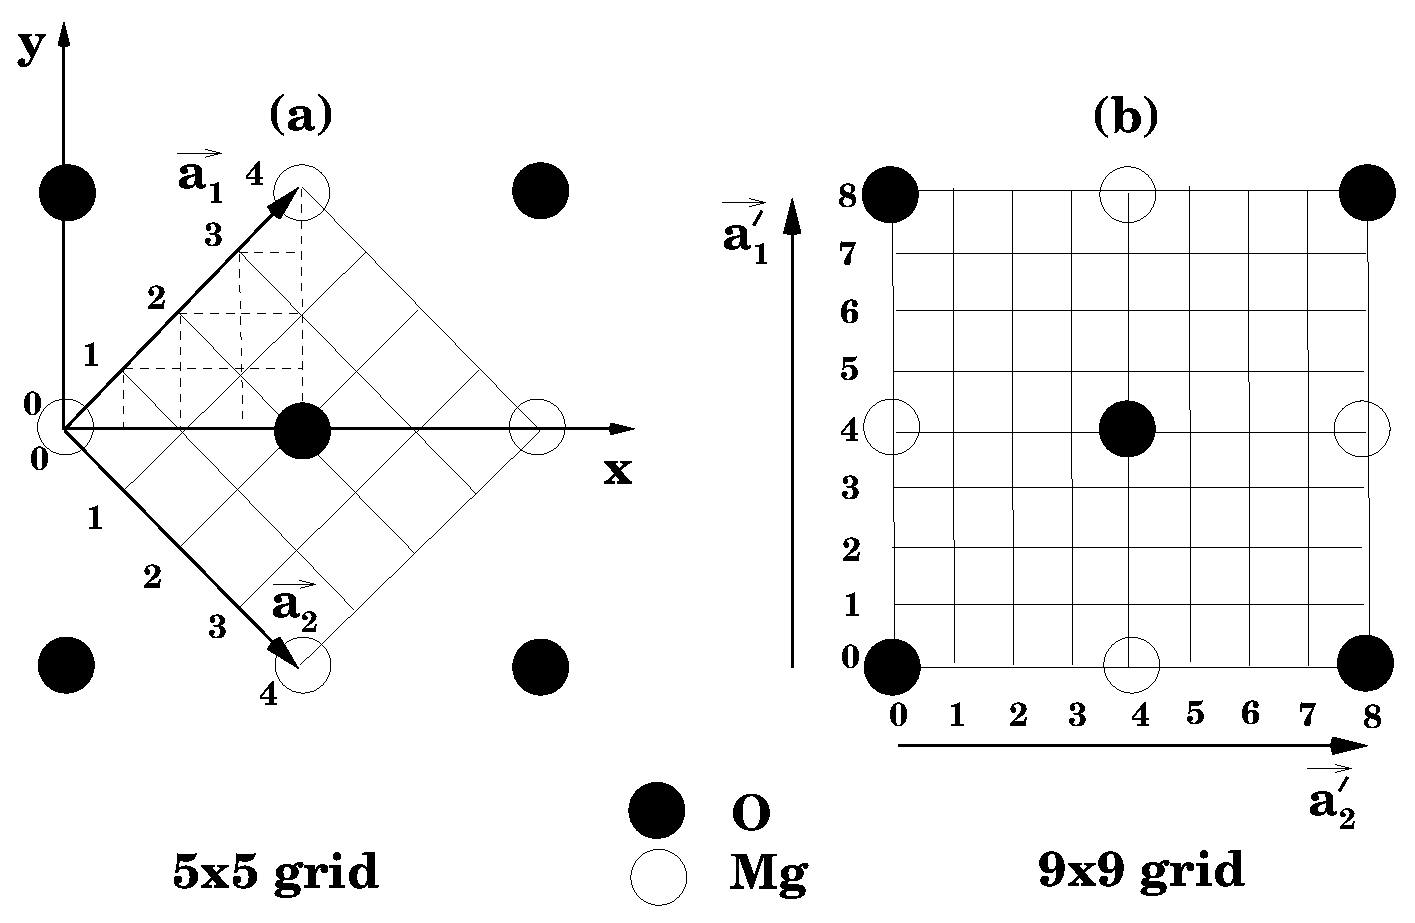
\includegraphics[%
  height=7cm]{xfig.grid.eps}\end{center}


\caption{How the force field can be specified for the MgO (001) surface: (a)
in the case of the 5x5 grid, the lattice vectors$\mathbf{a}_{1}$and
$\mathbf{a}_{2}$ correspond to the primitive unit cell; (b) in the
case of the 9x9 grid, a two times larger cell is chosen with the lattice
vectors $\mathbf{a}_{1}^{\prime}=\mathbf{a}_{1}-\mathbf{a}_{2}$ and
$\mathbf{a}_{2}^{\prime}=\mathbf{a}_{1}+\mathbf{a}_{2}$. The original
grid used to calculate the force field in non-equilvalent points in
the primitive cell is shown by dashed lines in (a). \label{cap:grid-for-force}}
\end{figure}
. In the directory \texttt{examples/MgO/force\_field} you can also
find raw data for the MgO force field calculated using the Sci-Fi
code. The calculations were performed using a 64 atom 4x4x4 MgO cube
tip with a Mg atom at the tip apex. The raw data for the force field
are set in directories 

\texttt{\textbackslash{}X=0,Y=0},

\texttt{\textbackslash{}X=0.5305,Y=0.5305,}

\texttt{\textbackslash{}X=0,Y=2.122},

\begin{flushleft}etc., corresponding to different values of the $X$
and $Y$ within the primitive cell as shown by the dashed lines in
Fig. \ref{cap:grid-for-force} (a). The coordinate axes are those
shown in Fig. \ref{cap:grid-for-force}, and the Mg-O distance is
equal to 2.122 \AA. The results of the calculation for a 2D scan
using either of the force field are collected in directories \texttt{examples/MgO/results\_5x5}
and \texttt{examples/MgO/results\_9x9} (see also section \ref{sub:2Dimage_S.dat}).\end{flushleft}

The information in the box is provided in the same way as in the previous
case: each time a keyword is used which is followed by the necessary
parameters. The order of each input is arbitrary, the order within
each input is fixed. 

\textbf{Important}: contrary to all other boxes, all values here are
provided using eV and \AA$\,$ units!!!


\subsubsection{How to specify the short-range force\label{sub:How-to-specify-short-range-force}}


\subsubsection*{\noindent Force\_field\_file}

Name of the file containing the short-range component of the force
field. Must only be supplied if the vAFM to be run without SciFi.

\begin{flushleft}\emph{Parameters}: filename (up to 50 characters)\end{flushleft}

\begin{flushleft}\emph{Default}: empty name\end{flushleft}

\noindent \emph{Example}: \texttt{\footnotesize Force\_field\_file
CaCO3.dat}{\footnotesize \par}


\subsubsection*{Pixels\{1,2,z\} }

Number of grid points $N_{1}$ and $N_{2}$ along directions $\mathbf{a}_{1}$
and $\mathbf{a}_{2}$, respectively, followed by the number $N_{z}$
of points along $z$.

\begin{flushleft}\emph{Parameters}: $N_{1}$, $N_{2}$, $N_{z}$\end{flushleft}

\begin{flushleft}\emph{Default}: 1,1,44\end{flushleft}

\noindent \emph{Example}: \texttt{\footnotesize Pixels\{1,2,z\} 25
49 44}{\footnotesize \par}


\subsubsection*{Lattice\{/A1(xy),/A2(xy)\} }

Components along $X$ and $Y$ axes of the laboratory Cartesian system
of the lattice vectors $\mathbf{a}_{1}$ and $\mathbf{a}_{2}$ are
given (in \AA) in two lines coming next after the keyword: $a_{1x}$,
$a_{1y}$ on the first and $a_{2x}$, $a_{2y}$ on the second.

\begin{flushleft}\emph{Default}: none\end{flushleft}

\noindent \emph{Example}: Lattice\{/A1(xy),/A2(xy)\}

\noindent \texttt{\footnotesize $\,\,\,\,\,\,\,\,\,\,$ 1.0 0.0 }{\footnotesize \par}

\noindent \texttt{\footnotesize $\,\,\,\,\,\,\,\,\,\,$ 0.0 1.0 }{\footnotesize \par}


\subsubsection{Long-range part of the force}


\subsubsection*{Long-Range\{bound,z0,g0,...,g6\}}

The parameters of the long-range part of the chemical force, Eq. (\ref{eq:long_range_force}),
are given using the \AA/eV units, so that the force would be in eV/\AA$\,$
and distances in \AA. 

\begin{flushleft}\emph{Parameters}: $z_{bound}$, $z_{0}$, $g_{0}$,
$g_{1}$,...,$g_{6}$\end{flushleft}

\begin{flushleft}\emph{Default}: 16.0, -5.0928, 0.0, 0.0, 0.0, -0.40916,
0.0, 0.0, 0.0 \end{flushleft}

\noindent \emph{Example}: \texttt{\footnotesize Long-Range\{bound,z0,g0,...,g6\}16.0
-5.0928 0.0 0.0 0.0 -0.40916 0.0 0.0 0.0}{\footnotesize \par}


\subsubsection*{vdW\{H,R\}}

Parameters for the vdW force (the force is in eV/\AA) as in Eq. (\ref{eq:vdw}).

\begin{flushleft}\emph{Parameters}: $H$, $R$\end{flushleft}

\begin{flushleft}\emph{Default}: 0.99864, 300.0\end{flushleft}

\noindent \emph{Example}: \texttt{\footnotesize vdW\{H,R\} 0.99864
300.0 }{\footnotesize \par}


\subsubsection{{*}Parameters necessary to run vAFM and SciFi together}


\subsubsection*{Atom\_Sphere\{\#,dist\}}

Paramaters for placing the vdW sphere within the atomistic part; only
needed if vAFM and SciFi are to work together. Should specify two
parameters: (i) atom number which is used to measure the distance
to the vdW sphere, $I$, and the distance $D$ (in $\textrm{�}$)
to the bottom of the vdW sphere from this atom.

\begin{flushleft}\emph{Parameters}: $I$, $D$\end{flushleft}

\begin{flushleft}\emph{Default}: 1, 0.0\end{flushleft}

\noindent \emph{Example}: \texttt{\footnotesize Atom\_Sphere\{\#,dist
15 1.25 }{\footnotesize \par}


\subsubsection*{interpolate\{F/T,points\}}

Two parameters are supplied: a logical (False or True) and the number
of points $N$. If the first variable is False, then no interpolation
of the tip force is done, it will be calculated at each tip position
by running full SciFi ionic relaxation calculation. If, however, the
first parameter is True, then an interpolation of the force between
two nearest known values (for vertical positions of the tip only)
will be done, atomic relaxation will not be performed saving computer
time. 

The parameter $N$specifies the number of nearest forces to be used
in the interpolation (only $N=2$is presently implemented).

\begin{flushleft}\emph{Parameters}: F, $N$~~~or~~~T, $N$\end{flushleft}

\begin{flushleft}\emph{Default}: T,2\end{flushleft}

\noindent \emph{Example}: \texttt{\footnotesize Force\_Test 0.01}{\footnotesize \par}


\subsubsection*{extrapolate\{F/T,polyn,points\}}

This option is supposed to control extrapolation of the tip force
- not yet implemented. The first parameter is F (do not apply) or
T (do apply extrapolation mechanism to the tip force), then the order
of a polynomial $N_{1}$ to be used for the extrapolation, and , finally,
the number of points $N_{2}$.

\begin{flushleft}\emph{Parameters}: F, $N_{1}$, $N_{2}$~~~or~~~T,
$N_{1}$, $N_{2}$\end{flushleft}

\begin{flushleft}\emph{Default}: T,2,3\end{flushleft}

\noindent \emph{Example}: \texttt{\footnotesize Fextrapolate\{F/T,polyn,points\}
T 2 3}{\footnotesize \par}


\subsubsection*{smooth\{F/T,points\}}

Controls smoothing out the forces using a certain number of points,
$N_{s}$.

\begin{flushleft}\emph{Parameters}: F, $N_{s}$~~~or~~~T, $N_{s}$\end{flushleft}

\begin{flushleft}\emph{Default}: T,2\end{flushleft}

\noindent \emph{Example}: \texttt{\footnotesize smooth\{F/T,points\}
T 2}{\footnotesize \par}


\subsubsection{Testing the whole range force field\label{sub:Testing-the-whole}}


\subsubsection*{Force\_Test }

The force field can be tested prior to (and instead of) any calculation
if $N_{ft}=$T is used as the first parameter; the second parameter
in this case is a step, $\Delta z$, along the $z$ direction (in
\AA). 

\begin{flushleft}\emph{Parameters}: $N_{ft}$, $\Delta z$\end{flushleft}

\begin{flushleft}\emph{Default}: F, 0.01\end{flushleft}

\noindent \emph{Example}: \texttt{\footnotesize Force\_Test 0.01}{\footnotesize \par}


\subsubsection{Structure of the force-field file\label{sub:Structure-of-the-force-file}}

Only relelvant if the force field file is specified, i.e. if the SciFi
part is switched off.

The short-range part of the force field is specified in a file as
was mentioned in section \ref{sub:How-to-specify-short-range-force}
above. Let us assume that the lateral grid is $N_{1}$, $N_{2}$ and
the number of points along the $Z$ axis is $N_{z}$. Then, the format
of this file is as follows:

\begin{itemize}
\item the 1st line: comment
\item $N_{z}$ lines follow with the $z$ values (in the ascending order)
\item a comment line
\item then the force field for every $i$, $j$ along the lateral grid mesh
follows in blocks as given by the following FORTRAN statement: 
\end{itemize}
\noindent \begin{center}\texttt{\footnotesize do i=0,N1}\end{center}{\footnotesize \par}

\noindent \begin{center}\texttt{\footnotesize ~~~do j=0,N2}\end{center}{\footnotesize \par}

\noindent \begin{center}\texttt{\footnotesize ~~~~~~..................}\end{center}{\footnotesize \par}

\noindent \begin{center}\texttt{\footnotesize ~~~end do}\end{center}{\footnotesize \par}

\noindent \begin{center}\texttt{\footnotesize end do}\end{center}{\footnotesize \par}

\begin{itemize}
\item each block contains the values of the force for all values of $z$
(in the same order as the values of $z$ themselves, of course!),
and it starts with a comment line.
\end{itemize}

\subsection{Elementary Stages Box\label{sub:Elementary-Stages-Box}}

\textbf{\emph{Box Keyword}}: \texttt{.<Elementary\_Stages>}


\subsubsection{What controls every elementary stage?}

Parameters controlling every elementary stage are listed below:

\begin{itemize}
\item amplitude noise ON/OFF (logical);
\item force noise ON/OFF (logical)
\item ADC is ON/OFF (logical):

\begin{itemize}
\item if ON, then the $z$ distance is adjusted so that the frequency shift
$\Delta f$ could be maintained aproximately constant close to the
set value,$\Delta f$ (real);
\item if OFF, then the distance is kept exactly constant instead (constant
height mode); the frequency will change along the simulation, still
kept at resonance;
\end{itemize}
\item AGC is ON/OFF (logical):

\begin{itemize}
\item if ON, then gain control allows to keep the oscillation amplitude
approximately constant close to the set value, $A$ (real), by constantly
adjusting the excitation amplitude;
\item if OFF, then the excitation amplitude is kept exactly constant, whereas
the oscillation amplitude may change along the simulation;
\end{itemize}
\item velocities $v_{x}$ and $v_{y}$ along the $X$ and $Y$ axes, kept
constant during every elementary stage (two real);
\item a logical variable which switches ON/OFF the tip-surface force;
\item a logical variable which switches ON/OFF the excitation signal applied
to the cantilever;
\item a logical variable which switches ON/OFF the detailed printout during
each stage to be made into the file \texttt{stageM.out} (\texttt{M}
being the stage number); if ON, then there is also an integer vartiable
equal to the number of timesteps after which the printout will be
made;
\item finally, presently there are three ways in which each stage can be
terminated (a character variable):

\begin{itemize}
\item \texttt{'time'} followed by the time is seconds;
\item \texttt{'freq'}: the stage will run to meet the frequency shift setpoint
for this stage (up to an error of 0.5 Hz);
\item \texttt{'ampl'}: the stage will run to meet the oscillation amplitude
setpoint for this stage (up to an error of 0.1 \AA). 
\end{itemize}
\end{itemize}

\subsubsection{Specifying each elementary stage\label{sub:Specifying-each-elementary}}

Each elementary stage within the box is specified in a sub-box which
is started by a keyword:

\smallskip{}
\noindent \texttt{\_\{begin\_stage\}\_}
\smallskip{}

\begin{flushleft}followed by the {}``keyword + parameters'' structure
identical to other boxes; the sub-box ends if either the next \texttt{\_\{begin\_stage\}\_}
keyword is found (to start the next stage sub-box) or the \end{flushleft}

\smallskip{}
\noindent \texttt{.<End>}
\smallskip{}

\begin{flushleft}marker of the entire box is found. All the parameters
which control the execution of every stage are initially set to the
default values from the \texttt{<VirtualAFM>} box of section \ref{sub:Virtual-AFM-Box}.
Therefore, it is only necessary to give for each stage all those parameters
which are different from the default values. All the keywords and
their corresponding parameters are listed below.\end{flushleft}


\subsubsection*{Finish\{how,time\}}

Three methods to finish the stage (as above).

\begin{flushleft}\emph{Options}: 'time', 'freq', 'ampl'\end{flushleft}

\begin{flushleft}\emph{Parameters}: time $t$ (in s) when option 'time'
is used\end{flushleft}

\begin{flushleft}\emph{Default}: 'time' with 0.0 s\end{flushleft}

\noindent \emph{Examples}: \texttt{\footnotesize Finish\{how,time\}
time 0.01}{\footnotesize \par}

\noindent \texttt{\footnotesize ~~~~~~~~~~~~Finish\{how,time\}
freq}{\footnotesize \par}

\noindent \texttt{\footnotesize ~~~~~~~~~~~~Finish\{how,time\}
ampl}{\footnotesize \par}


\subsubsection*{Excite\{T/F\}}

Switches ON/OFF the excitation signal applied to the cantilever.

\begin{flushleft}\emph{Parameters}: F/T\end{flushleft}

\begin{flushleft}\emph{Default}: T\end{flushleft}

\noindent \emph{Example}: \texttt{\footnotesize EXcite\{T/F\} T}{\footnotesize \par}


\subsubsection*{ADC\{T/F,freq\}}

Switches ON/OFF the ADC; if ON, then the set point frequency shift
(negative) is also provided (in Hz). 

\begin{flushleft}\emph{Parameters}: F/T, $\Delta f$\end{flushleft}

\begin{flushleft}\emph{Default}: T, $\Delta f_{0}$\end{flushleft}

\noindent \emph{Example}: \texttt{\footnotesize ADC\{T/F,freq\} T
-100.0}{\footnotesize \par}


\subsubsection*{AGC\{T/F,A0\}}

Switches ON/OFF the AGC; if ON, then the set point amplitude $A$
is also provided (in m). 

\begin{flushleft}\emph{Parameters}: F/T, $A$\end{flushleft}

\begin{flushleft}\emph{Default}: T, $A_{0}$\end{flushleft}

\noindent \emph{Example}: \texttt{\footnotesize AGC\{T/F,A0\} T 0.1e-9}{\footnotesize \par}


\subsubsection*{Noise\{F,A\}}

Switches ON/OFF the noise for the force and the amplitude (in this
order).

\begin{flushleft}\emph{Parameters}: F/T, F/T\end{flushleft}

\begin{flushleft}\emph{Default}: as in \texttt{<VirtualAFM>} box\end{flushleft}

\noindent \emph{Example}: \texttt{\footnotesize Noise\{F,A\} T T}{\footnotesize \par}


\subsubsection*{Prt\{T/F,how\_often\}}

Switches the detailed printing ON/OFF; if ON, then it prints a number
of essential variables along the simulation into the file \texttt{stageM.out}
(\texttt{M} being the stage number) every $M_{dt}$ timesteps.

\begin{flushleft}\emph{Parameters}: F/T, $M_{dt}$\end{flushleft}

\begin{flushleft}\emph{Default}: as in \texttt{<VirtualAFM>} box\end{flushleft}

\noindent \emph{Example}: \texttt{\footnotesize Prt\{T/F,how\_often\}
T 10}{\footnotesize \par}


\subsubsection*{Velocity\{Vx,Vy\}}

Sets velocities $v_{x}$ and $v_{y}$ along the $X$ and $Y$ directions
(in m/s) for the given stage.

\begin{flushleft}\emph{Parameters}: $v_{x}$, $v_{y}$\end{flushleft}

\begin{flushleft}\emph{Default}: 0.0, 0.0\end{flushleft}

\noindent \emph{Example}: \texttt{\footnotesize Velocity\{Vx,Vy\}
0.0e0 1.0e-9}{\footnotesize \par}


\subsubsection*{Tip\_Force\{T/F\}}

Switches ON/OFF the tip-surface force. 

\begin{flushleft}\emph{Parameters}: T/F\end{flushleft}

\begin{flushleft}\emph{Default}: T\end{flushleft}

\noindent \emph{Example}: \texttt{\footnotesize Tip\_Force\{T/F\}
T}{\footnotesize \par}


\subsubsection{Doing a 2D scan}

Using elementary stages as described above one can program in any
particular movement of the cantilever across the surface including
doing a 2D scan. This last option may be tedious though since many
times the same pattern of line scans should be repeated. To avoid
this, the 2D scan can be automated using another sub-box structure
inside the \texttt{<Elementary\_Stages>} box. 

The basic idea is that a 2D scan can be simulated by repeating e.g.
4 elementary stages: 

\begin{enumerate}
\item a line scan along direction $\mathbf{b}_{1}$ during a long time $t_{1}$
\item a line scan along the perpendicular direction $\mathbf{b}_{2}$ during
a very short time $t_{2}$
\item a line scan along direction $-\mathbf{b}_{1}$ during time $t_{1}$
\item a line scan along the perpendicular direction $\mathbf{b}_{2}$ during
a very short time $t_{2}$
\end{enumerate}
Some other possibilities for a 2D scan also exist, e.g. by repeating
only 3 stages:

\begin{enumerate}
\item a line scan along direction $\mathbf{b}_{1}$ during a long time $t_{1}$
\item a line scan along direction $-\mathbf{b}_{1}$ during the same time
$t_{1}$
\item a line scan along the perpendicular direction $\mathbf{b}_{2}$ during
a very short time $t_{2}$
\end{enumerate}
Thus any scan can be viewed as an identical sequence of structures,
each consisting of several elementary stages. The number of sequences
determines the length of the scan in the direction $\mathbf{b}_{2}$,
whereas the length of the scan in the perpendicular direction $\mathbf{b}_{1}$
is determined by the time $t_{1}$ in the examples above. 

It is possible to position the scan sub-box arbitrarily between any
stage sub-boxes inside the \texttt{<Elementary\_Stages>} box as shown
in the example in section \ref{sub:Example-Input-File}. Therefore,
it is possible to do some number of elementary stages, then a scan,
then some other elementary stages, another scan, etc. The total length
of this chain of stages is only limited by the maximum number of stages
and scans allowed as given by the two parameters in the \texttt{virtual\_param.inc}
file (see section \ref{sub:virtual_param.inc-file}). Note that every
scan is eventually constructed as a set of stages, so that the parameter
\texttt{N\_of\_stages\_max} can easily become too small and need to
be increased, and the code recompiled. 

To start a scan, place the keyword 

\smallskip{}
\noindent \begin{flushleft}\texttt{===\{begin\_scan\}===}\end{flushleft}
\smallskip{}

\noindent \begin{flushleft}after a stage sub-box%
\footnote{Note that you have to do the approach anyway, so that the stage sub-box
should always precede any of the scan boxes.%
}. The next line \emph{should} contain the {}``keyword + parameter''
structure: \end{flushleft}


\subsubsection*{\noindent No\_of\_sequences}

\begin{flushleft}\emph{Parameters}: number of sequences\end{flushleft}

\begin{flushleft}\emph{Default}: none\end{flushleft}

\noindent \begin{flushleft}\emph{Example}: \texttt{\footnotesize No\_of\_sequences
100}\end{flushleft}{\footnotesize \par}
\smallskip{}

\noindent \begin{flushleft}This parameter defines the number of times
each sequence is to be repeated. After that, the elementary sequence,
consisiting of elementary passages (i.e. stages) follows in the same
way as described in section \ref{sub:Specifying-each-elementary}.
The scan sub-box is terminated with the keyword\end{flushleft}

\smallskip{}
\noindent \begin{flushleft}\texttt{===\{end\_scan\}===}\end{flushleft}
\smallskip{}

\noindent \begin{flushleft}For instance, the 4-stage/passage scan
structure to be repeated 10 times along the $X$ direction is given
by the following scan sub-box:\end{flushleft}
\smallskip{}

\texttt{\footnotesize ===\{begin\_scan\}===}{\footnotesize \par}

\texttt{\footnotesize No\_of\_sequences 10}{\footnotesize \par}

\texttt{\footnotesize \_\{begin\_stage\}\_}{\footnotesize \par}

\texttt{\footnotesize Finish\{how,time\} time 0.01}{\footnotesize \par}

\texttt{\footnotesize Velocity\{Vx,Vy\} 0.0 1.0e-9}{\footnotesize \par}

\texttt{\footnotesize ADC\{T/F,freq\} T -440.0}{\footnotesize \par}

\texttt{\footnotesize \_\{begin\_stage\}\_}{\footnotesize \par}

\texttt{\footnotesize Finish\{how,time\} time 0.001}{\footnotesize \par}

\texttt{\footnotesize Velocity\{Vx,Vy\} 1.0e-9 0.0}{\footnotesize \par}

\texttt{\footnotesize ADC\{T/F,freq\} T -440.0}{\footnotesize \par}

\texttt{\footnotesize \_\{begin\_stage\}\_}{\footnotesize \par}

\texttt{\footnotesize Finish\{how,time\} time 0.01}{\footnotesize \par}

\texttt{\footnotesize Velocity\{Vx,Vy\} 0.0 -1.0e-9}{\footnotesize \par}

\texttt{\footnotesize ADC\{T/F,freq\} T -440.0}{\footnotesize \par}

\texttt{\footnotesize \_\{begin\_stage\}\_}{\footnotesize \par}

\texttt{\footnotesize Finish\{how,time\} time 0.001}{\footnotesize \par}

\texttt{\footnotesize Velocity\{Vx,Vy\} 1.0e-9 0.0}{\footnotesize \par}

\texttt{\footnotesize ADC\{T/F,freq\} T -440.0}{\footnotesize \par}

\texttt{\footnotesize ===\{end\_scan\}===}{\footnotesize \par}

\smallskip{}
\noindent Here $\Delta f$ is set to -440 Hz during the whole scan. 


\newpage
\part{Output}


\section{SciFi specific output}


\subsection{Standard Output}

The output to the screen will tell you the main parameters for your
calculation and will also warn you of any obvious inconsistencies
that the program is trying to compensate for. If there are any major
problems with the input the program will exit with a fatal error and
a message explaining the nature of the error.


\subsection{Output File}

Every run will produce an output file called \texttt{name.OUT}, this
will contain detailed information (depending on the printing parameter)
about your system and the calculations run on it. The first stage
of the output file will give all the input parameters as recognized
by the program followed by some basic information about your system
derived from those parameters. This is the first place to check for
consistency, make sure that the output is consistent with the system
you intended in your input. The rest of the output file will detail
the process of the calculations, including a display of the total
energy and all forces (and the source of those forces) on the atoms
at each relaxation iteration. If an energy minimisation calculation
is being performed, then at the end of the file the total force on
the tip (if there was one) will be displayed along with a total force
breakdown. 


\subsection{Configuration Files}

If a minimisation calculation is being performed and the \textbf{xyz}
option is present in the Toleranc box, then the program will produce
two \texttt{.xyz} format files: \texttt{name\_core.xyz} and \texttt{name\_shell.xyz},
containing the final relaxed coordinates of the cores and shells in
the system correspondingly. If a scan is performed using the energy
minimisation method (i.e. the TipDynamics box is present), the two
files will contain coordinates of cores and shells at every point
at the tip path one after another.


\subsection{Statistics File}

If a Molecular Dynamics simulation is being performed, the run will
produce a file with thermodynamic data at intervals set with the \textbf{statistics}
variable, with the filename \texttt{name.STS}. This file constists
of a line for every interval, split into six columns that give: timestep,
total system energy, potential energy, kinetic energy, temperature
and shell temperature. 

The same file is also produced during a scan made using options in
the TipDynamics box. If only energy minimisation is performed (the
box MDcontrol is absent) and the tip is allowed to move (the TipDynamics
box is present), the file will contain only total energies of the
system at every scan point.


\subsection{Trajectory File}

An MD run will produce a trajectory file named \texttt{name.TRJ} of
the format and interval specified in the MDcontrol box. This file
contains the atomic coordinates of the system at each interval. 


\subsection{Tip Force Files}

If a Molecular Dynamics simulation is being peformed, then the run
will produce a file with the total z-component of the force on the
tip at every timestep called \texttt{name.TFZ}. If the the \textbf{do\_lat}
flag is used in the MDcontrol box, then x- and y-components of the
total force on the tip at every timestep will be written to the files
\texttt{name.TFX} and \texttt{name.TFY} respectively. 

The same files are produced during a scan (i.e. when the TipDynamics
box is present) if only energy minimisation is performed (the box
MDcontrol is absent).


\subsection{Output from \texttt{image}}

If the image input box is activated correctly then the image interaction
in your system will be calculated and several other output files will
be produced. In general it is not necessary to look at these, but
they are useful for detailed analysis of the image force and also
for finding the source of any strange behaviour in the calculations.
The possible files produced are as follows:

\begin{itemize}
\item \emph{charges.out} - which contains the position (in a.u.) and charge
of every image charge created (if \textbf{qwrite} is on).
\item \emph{forces.out} - which contains the image force on every atom (excluding
the \textbf{frozen-tip} atoms) and the total image force.
\item \emph{image.out} - which contains an output of the parameters used
in calculating the image force.
\item \emph{out} - standard output from calculating image force on atoms.
\item \emph{outf} - standard output from calculating the image force on
the tip.
\item \emph{potent.out} - which contains the image potential on all atoms
in the system and the image energy.
\end{itemize}

\section{vAFM specific output\label{sec:vAFM-specific-output}}

The output to the screen will tell you the main parameters for your
calculation and will also show the processing of each elementary stage.
In adition, a number of output files are produced.


\subsection{\texttt{\normalsize virtual.out}}

This files starts with detailed information concerning with the current
calculation. In particular, it contains a detailed account of all
the stages made of both individual stages and 2D scans, in a form
of a table. After the input part, it gives some useful information
about each stage in the process of the calculation, specifically about
the setpoints and the initial values of some variables. An example
of this file is given in the directory \texttt{/examples} for the
input file of section \ref{sub:Example-Input-File}. 


\subsection{\texttt{\normalsize stageM.out}}

\noindent This type of file with \texttt{M} being the stage number
is created at every stage provided that the detailed printing is ON.
The file starts from the heading which explains the variables it contains:
\smallskip{}

\texttt{\footnotesize \# excite - excitation signal at timestep t }{\footnotesize \par}

\texttt{\footnotesize \# DEF - frequency shift (Hz) }{\footnotesize \par}

\texttt{\footnotesize \# ds - distance of closest approach (A) }{\footnotesize \par}

\texttt{\footnotesize \# dist - actual distance at time t (A)}{\footnotesize \par}

\texttt{\footnotesize \# ftip - force (eV/A)}{\footnotesize \par}

\texttt{\footnotesize \# A - oscillation amplitude }{\footnotesize \par}

\texttt{\footnotesize \#}{\footnotesize \par}

\texttt{\footnotesize \# t ~~~~~~ z(t)~~~~~~ excite~~~~~
DEF~~~~~ ds~~~~~ ftip~~~~~ dist~~~~ A }{\footnotesize \par}

\smallskip{}
\noindent Note that variables printed out during the first two stages
are slightly different.


\subsection{\texttt{\normalsize signals.dat}}

\noindent This single file contains the output (in the correct order
of stages) in the following form: 
\smallskip{}

\texttt{\footnotesize \# oscil - oscillation number}{\footnotesize \par}

\texttt{\footnotesize \# X,Y - lateral position (in A) }{\footnotesize \par}

\texttt{\footnotesize \# A - oscillation amplitude (in A) }{\footnotesize \par}

\texttt{\footnotesize \# DEF - frequency shift (Hz) }{\footnotesize \par}

\texttt{\footnotesize \# Ediss - dissipation energy per cycle (eV) }{\footnotesize \par}

\texttt{\footnotesize \# appr - distance of closest approach (A) }{\footnotesize \par}

\texttt{\footnotesize \# }{\footnotesize \par}

\texttt{\footnotesize \# ~~~oscil~~~ X~~~~ Y~~~~ A~~~~
DEF~~~~ Ediss~~~~ appr }{\footnotesize \par}

\smallskip{}
\noindent Variables printed into the file are calculated every $N$-th
oscillation cycle at the end of the oscillation period (when the tip
is at the top most position). Here $N$ is the parameter specified
after the keyword \texttt{Print\_Cycles}, section \ref{sub:The-frequency-of-gen-printout}.


\subsection{\noindent \texttt{\normalsize 2Dimage\_S.dat\label{sub:2Dimage_S.dat}}}

\noindent For each scan a file with this name is produced (\texttt{S}
is the scan number), which contains:
\smallskip{}

\texttt{\footnotesize \# X,Y - lateral position (in A) }{\footnotesize \par}

\texttt{\footnotesize \# A - oscillation amplitude (in A) }{\footnotesize \par}

\texttt{\footnotesize \# DEF - frequency shift (Hz) }{\footnotesize \par}

\texttt{\footnotesize \# Ediss - dissipation energy per cycle (eV) }{\footnotesize \par}

\texttt{\footnotesize \# appr - distance of closest approach (A) }{\footnotesize \par}

\texttt{\footnotesize \# }{\footnotesize \par}

\texttt{\footnotesize \# ~~~ X~~~~ Y~~~~ A~~~~ DEF~~~~
Ediss~~~~ appr }{\footnotesize \par}

Difference with the \texttt{singnal.dat} file is two-fold: firstly,
the oscillation number is not printed; secondly, different files are
produced for each stage.

As an example, we show in Fig. \ref{cap:2D-topography-image} the
2D topology image of the MgO (001) surface calculated by the code
using the 9x9 force field (section \ref{sub:Force-Field-Box}). %
\begin{figure}[!ht]
\begin{center}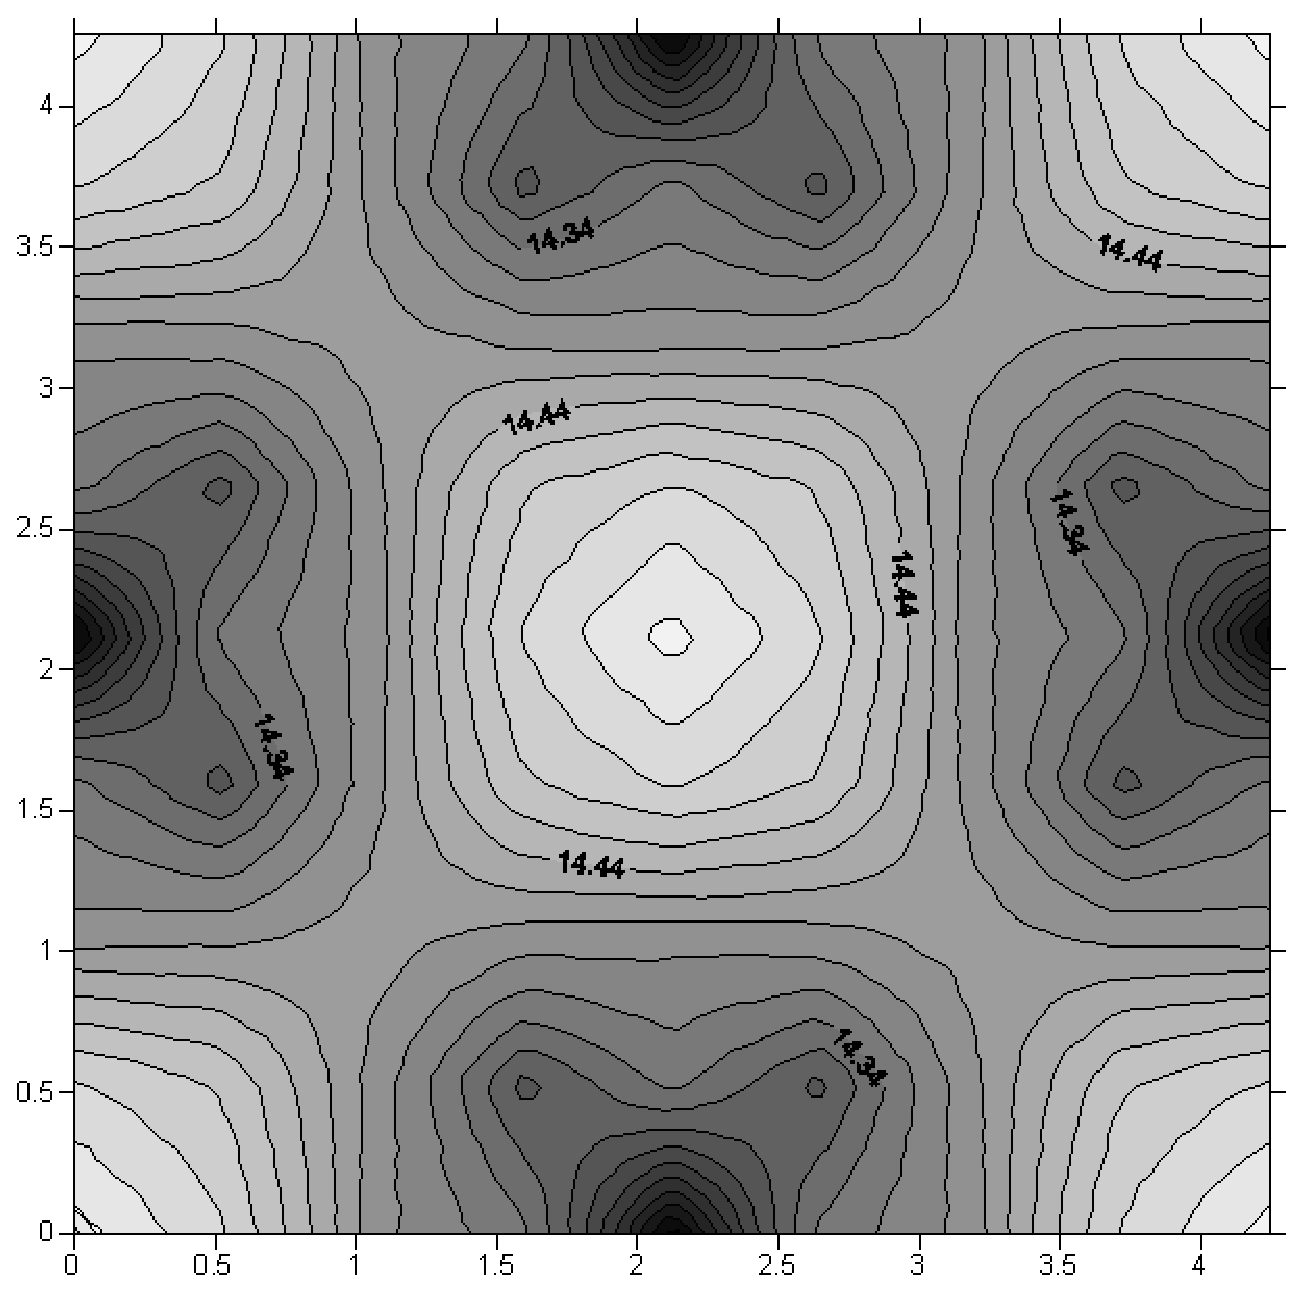
\includegraphics[%
  height=8cm]{9x9.eps}\end{center}


\caption{2D topography image of the MgO (001) surface calculate using the
9x9 grid force field.\label{cap:2D-topography-image}}
\end{figure}
 Black spots correspond to Mg atoms, while white ones - to O atoms.
The force field was obtained using a 64 atom 4x4x4 MgO cube with a
Mg atom at the tip apex. This is in perfect qualitative agreement
with the image shown. 


\subsection{\texttt{\normalsize ftip.dat}}

This file is produced if the tip force is tested (section \ref{sub:Testing-the-whole}).
Its heading reflects its contents:

\texttt{\footnotesize \# force field for given X,Y=( 0.00000, 0.00000) }{\footnotesize \par}

\texttt{\footnotesize \#~~~~ z (in A) ~~~~~vdW (in eV/A)~~~~~~~
chemical (in e/V)~~~~~ total (in eV/A) }{\footnotesize \par}


\newpage
\part{Example Inputs\label{Sec::Example-Inputs}}

A large number of input files are contained in the subdirectory \texttt{examples}
together with corresponding output files. The directory is broken
down into three subdirectories corresponding to 

\begin{enumerate}
\item SciFi only runs
\item vAFM only runs
\item SciFi+vAFM runs: in this case only approach has been modelled, i.e.
the same lateral position of the tip has been used
\end{enumerate}
Most of the examples are based on an insulating MgO surface interacting
with a model 64 atom cube MgO tip, e.g.

\begin{itemize}
\item mgo.INN - MD simulations of an insulating MgO tip interacting with
a MgO sample
\item mgo1.INN - test of the tip force for an insulating tip interacting
with cluster
\item mgo\_mt.INN - lateral scan of an MgO tip above the MgO sample.
\end{itemize}
\bibliographystyle{unsrt}
\bibliography{mypapers,spm,manipulation,virtual}

\end{document}
